
%\documentclass[manuscript]{acmart}
%\documentclass[acmsmall]{acmart}
%\settopmatter{printacmref=false}


\documentclass[
  a4paper,
  12pt,
  DIV=12,        % höherer Wert = schmalere Ränder, weniger Whitespacmi
  parskip=half,  % Absätze mit halbem Abstand statt Einzug
  headings=small % kleinere Überschriften, weniger vertikaler Abstand
]{scrartcl}

%\documentclass[a4paper,11pt]{scrartcl}
%\documentclass[a4paper,11pt]{report}
%\documentclass[a4paper,12pt]{book}
\usepackage[utf8]{inputenc}
\usepackage[german]{babel}
\usepackage[T1]{fontenc}
\usepackage{lmodern}
\usepackage[inkscapelatex=false]{svg}

\DeclareUnicodeCharacter{2502}{|}
\DeclareUnicodeCharacter{251C}{+}
\DeclareUnicodeCharacter{2514}{+}
\DeclareUnicodeCharacter{2500}{-}
\DeclareUnicodeCharacter{03B8}{\ensuremath{\theta}}
% Texte im SVG von Inkscape setzen lassen, nicht durch die Dokumentschrift ersetzen
\svgsetup{inkscapelatex=false}
\usepackage{amsmath}
\usepackage{caption}
\usepackage{gensymb}
\usepackage{microtype}
\usepackage{longtable}
\usepackage{tabularx}   % Spalten, die die restliche Zeilenbreite auffüllen (X-Spalte)
\usepackage{booktabs}   % \toprule \midrule \bottomrule (in mobrob_table.tex verwendet)
\usepackage{wrapfig}    % Textumfluss um Abbildungen
\usepackage{array}
\usepackage{calc}

\usepackage[citecolor=black, colorlinks=true, linkcolor=black, urlcolor=blue]{hyperref}


%\usepackage{geometry}
\usepackage{siunitx}
%\geometry{margin=2.5cm}


\usepackage{amsthm}
\usepackage{mdframed}
\usepackage{enumitem}

\newmdtheoremenv{theorem}{Theorem}

\theoremstyle{definition}
\newmdtheoremenv{derivation}{Derivation}

\providecommand{\tightlist}{%
  \setlength{\itemsep}{0pt}\setlength{\parskip}{0pt}}

%\mdfdefinestyle{leftline}{
%    topline=false, bottomline=false, rightline=false,
%    linewidth=2pt, linecolor=gray
%}
\theoremstyle{definition}
\newmdtheoremenv[style=leftline]{myalgorithm}{Algorithm}




%\usepackage{fancyvrb}







\let\Bbbk\relax
\usepackage{amssymb}


\usepackage{yfonts}

\usepackage{kvmap}

\usepackage[
    backend=biber,
    style=alphabetic,
    sortlocale=de_DE,
    natbib=true,
    %url=false,
    doi=true,
    %eprint=false
]{biblatex}
% \addbibresource{Literaturrecherche-Stefan-Etringer/algo-references.bib}

%\usepackage[
%    backend=biber,
%    style=alphabetic,
%    sortlocale=de_DE,
%    natbib=true,
%    %url=false,
%    doi=true,
%    %eprint=false
%]{biblatex}
%\addbibresource{Literaturrecherche-Dennis/mobrob_references.bib}

\usepackage[autostyle=true,german=quotes]{csquotes}
\usepackage{trfsigns} %fourier transform arrow
\usepackage{mathrsfs} %fourier F
\usepackage{commath}

\usepackage{pgfplots}
\pgfplotsset{compat=1.18}

\usepackage{xcolor}
\usepackage{listings}
\usepackage[european]{circuitikz}
\ctikzset{tripoles/european not symbol=ieee circle}

%\usepackage[shading]{moeptikz}
%\moeptikzset{shading=true}

%\usepackage{german,longtable}

\usepackage{xcolor}
\usepackage{color}
\usepackage{url}

\usepackage{xfrac}

\usepackage{listings}
\usepackage{verbatimbox}

\usepackage{algorithm}
\usepackage{algpseudocode}

\usepackage{multirow}
\usepackage{float}
\usepackage{pdflscape}   % einzelne Querformatseiten (im PDF gedreht)

%%%% TIKZ

\usepackage{tikz}

\usepackage{pgfplots}
\usetikzlibrary{calc,
trees,positioning,arrows,
chains,shapes.geometric,
decorations.pathreplacing,
decorations.pathmorphing,shapes,
matrix,shapes.symbols,
plotmarks}
%\tikzexternalize[prefix=figures/]

%\tikzset{%
%  block/.style    = {draw, thick, rectangle, minimum height = 3em,
%    minimum width = 3em},
%  sum/.style      = {draw, circle, node distance = 2cm}, % Adder
%  input/.style    = {coordinate}, % Input
%  output/.style   = {coordinate} % Output
%}
% Defining string as labels of certain blocks.
%\newcommand{\suma}{\Large$+$}
%\newcommand{\multa}{\Large$\times$}
%\newcommand{\inte}{$\displaystyle \int$}
%\newcommand{\derv}{\huge$\frac{d}{dt}$}

\usetikzlibrary{arrows,automata,positioning}
%\usepackage{automata}


%%% END TIKZ

\usepackage[section]{placeins}

\usepackage{textcomp}


\usepackage{listings}
\usepackage{verbatimbox}

\usepackage{bold-extra}

\usepackage{framed}
\usepackage{color}
\usepackage{fancyvrb}
\newcommand{\VerbBar}{|}
\newcommand{\VERB}{\Verb[commandchars=\\\{\}]}
\DefineVerbatimEnvironment{Highlighting}{Verbatim}{commandchars=\\\{\}}
% Add ',fontsize=\small' for more characters per line
\newenvironment{Shaded}{}{}
\newcommand{\AlertTok}[1]{\textcolor[rgb]{1.00,0.00,0.00}{\textbf{#1}}}
\newcommand{\AnnotationTok}[1]{\textcolor[rgb]{0.38,0.63,0.69}{\textbf{\textit{#1}}}}
\newcommand{\AttributeTok}[1]{\textcolor[rgb]{0.49,0.56,0.16}{#1}}
\newcommand{\BaseNTok}[1]{\textcolor[rgb]{0.25,0.63,0.44}{#1}}
\newcommand{\BuiltInTok}[1]{\textcolor[rgb]{0.00,0.50,0.00}{#1}}
\newcommand{\CharTok}[1]{\textcolor[rgb]{0.25,0.44,0.63}{#1}}
\newcommand{\CommentTok}[1]{\textcolor[rgb]{0.38,0.63,0.69}{\textit{#1}}}
\newcommand{\CommentVarTok}[1]{\textcolor[rgb]{0.38,0.63,0.69}{\textbf{\textit{#1}}}}
\newcommand{\ConstantTok}[1]{\textcolor[rgb]{0.53,0.00,0.00}{#1}}
\newcommand{\ControlFlowTok}[1]{\textcolor[rgb]{0.00,0.44,0.13}{\textbf{#1}}}
\newcommand{\DataTypeTok}[1]{\textcolor[rgb]{0.56,0.13,0.00}{#1}}
\newcommand{\DecValTok}[1]{\textcolor[rgb]{0.25,0.63,0.44}{#1}}
\newcommand{\DocumentationTok}[1]{\textcolor[rgb]{0.73,0.13,0.13}{\textit{#1}}}
\newcommand{\ErrorTok}[1]{\textcolor[rgb]{1.00,0.00,0.00}{\textbf{#1}}}
\newcommand{\ExtensionTok}[1]{#1}
\newcommand{\FloatTok}[1]{\textcolor[rgb]{0.25,0.63,0.44}{#1}}
\newcommand{\FunctionTok}[1]{\textcolor[rgb]{0.02,0.16,0.49}{#1}}
\newcommand{\ImportTok}[1]{\textcolor[rgb]{0.00,0.50,0.00}{\textbf{#1}}}
\newcommand{\InformationTok}[1]{\textcolor[rgb]{0.38,0.63,0.69}{\textbf{\textit{#1}}}}
\newcommand{\KeywordTok}[1]{\textcolor[rgb]{0.00,0.44,0.13}{\textbf{#1}}}
\newcommand{\NormalTok}[1]{#1}
\newcommand{\OperatorTok}[1]{\textcolor[rgb]{0.40,0.40,0.40}{#1}}
\newcommand{\OtherTok}[1]{\textcolor[rgb]{0.00,0.44,0.13}{#1}}
\newcommand{\PreprocessorTok}[1]{\textcolor[rgb]{0.74,0.48,0.00}{#1}}
\newcommand{\RegionMarkerTok}[1]{#1}
\newcommand{\SpecialCharTok}[1]{\textcolor[rgb]{0.25,0.44,0.63}{#1}}
\newcommand{\SpecialStringTok}[1]{\textcolor[rgb]{0.73,0.40,0.53}{#1}}
\newcommand{\StringTok}[1]{\textcolor[rgb]{0.25,0.44,0.63}{#1}}
\newcommand{\VariableTok}[1]{\textcolor[rgb]{0.10,0.09,0.49}{#1}}
\newcommand{\VerbatimStringTok}[1]{\textcolor[rgb]{0.25,0.44,0.63}{#1}}
\newcommand{\WarningTok}[1]{\textcolor[rgb]{0.38,0.63,0.69}{\textbf{\textit{#1}}}}
%\usepackage{fancyhdr}
%\pagestyle{fancy}
%\lhead{\leftmark}
%\chead{}
%\rhead{}
%\lfoot{}
%\cfoot{\thepage}
%\rfoot{}
%\renewcommand{\headrulewidth}{0.2pt}
%\renewcommand{\footrulewidth}{0.2pt}



\newcommand{\Z}{\mathbb{Z}}
\newcommand{\R}{\mathbb{R}}
\newcommand{\C}{\mathbb{C}}
\newcommand{\N}{\mathbb{N}}
\newcommand{\SqrtNy}{$\sqrt{\textsc{Ny}}$}
\newcommand{\conj}{\overline}
\newcommand{\Kset}{\textswab{K}}
\newcommand{\Qset}{\textswab{Q}}
\newcommand{\ceil}[1]{\left\lceil #1 \right\rceil}
\newcommand{\floor}[1]{\left\lfloor #1 \right\rfloor}
\newcommand{\sorted}[1]{\textsc{sort}\left\lbrace #1 \right\rbrace}
\newcommand{\SNRgain}{a_{SNR}}
\newcommand{\EQgain}{a_{EQ}}
\newcommand{\SIRgain}{a_{SIR}}
\newcommand{\SNIRgain}{a_{SINR}}
\newcommand{\SNR}{\textsc{SNR}}
\newcommand{\CIRgain}{a_{CIR}}
\newcommand{\CINRgain}{a_{CINR}}
\newcommand{\CNR}{\textsc{CNR}}
\newcommand{\CINR}{\textsc{CINR}}
\newcommand{\HPAModel}{ Hughes 1177H TWTA }
\newcommand{\bigO}{\mathcal{O}}
\newcommand{\CopWinCompl}{2.375377}
\newcommand{\IBO}{\textsc{IBO}}
\newcommand{\OBO}{\textsc{OBO}}
\newcommand{\spacepage}{\newpage\null\thispagestyle{empty}\newpage}
\newcommand{\satcom}{ SatCom }
\newcommand{\db}{~\text{dB}}


\definecolor{mGreen}{rgb}{0,0.6,0}
\definecolor{mGray}{rgb}{0.5,0.5,0.5}
\definecolor{mPurple}{rgb}{0.58,0,0.82}
\definecolor{backgroundColour}{rgb}{0.95,0.95,0.92}

\lstdefinestyle{CStyle}{
    backgroundcolor=\color{backgroundColour},
    commentstyle=\color{mGreen},
    keywordstyle=\color{magenta},
    numberstyle=\tiny\color{mGray},
    stringstyle=\color{mPurple},
    basicstyle=\footnotesize,
    breakatwhitespace=false,
    breaklines=true,
    captionpos=b,
    keepspaces=true,
    numbers=left,
    numbersep=5pt,
    showspaces=false,
    showstringspaces=false,
    showtabs=false,
    tabsize=2,
    language=C
}

\lstdefinelanguage{VHDL}{
  morekeywords=[1]{library,use,all,entity,is,port,in,out,end,architecture,of,begin,process,if,then,else,elsif,when,others,signal,variable,wait,for,loop},
  morecomment=[l]--,
  morestring=[b]",
  sensitive=true
}

\lstset{
  language=VHDL,
  basicstyle=\ttfamily\small,
  keywordstyle=\color{blue},
  commentstyle=\color{gray},
  stringstyle=\color{red},
  numbers=left,
  numberstyle=\tiny,
  stepnumber=1,
  numbersep=8pt,
  frame=single,
  breaklines=true,
  captionpos=b
}

\lstset{numbers=none}

%\newcounter{example}
%\renewcommand{\theexample}{\thesection.\arabic{example}}


% Default fixed font does not support bold face
\DeclareFixedFont{\ttb}{T1}{txtt}{bx}{n}{12} % for bold
\DeclareFixedFont{\ttm}{T1}{txtt}{m}{n}{12}  % for normal

% Custom colors
\usepackage{color}
\definecolor{deepblue}{rgb}{0,0,0.5}
\definecolor{deepred}{rgb}{0.6,0,0}
\definecolor{deepgreen}{rgb}{0,0.5,0}

\usepackage{listings}

% Python style for highlighting
\newcommand\pythonstyle{\lstset{
language=Python,
basicstyle=\ttm,
morekeywords={self},              % Add keywords here
keywordstyle=\ttb\color{deepblue},
emph={MyClass,__init__},          % Custom highlighting
emphstyle=\ttb\color{deepred},    % Custom highlighting style
stringstyle=\color{deepgreen},
frame=tb,                         % Any extra options here
showstringspaces=false
}}


% Python environment
\lstnewenvironment{python}[1][]
{
\pythonstyle
\lstset{#1}
}
{}

% Python for external files
\newcommand\pythonexternal[2][]{{
\pythonstyle
\lstinputlisting[#1]{#2}}}

% Python for inline
\newcommand\pythoninline[1]{{\pythonstyle\lstinline!#1!}}





\nocite{*}


\begin{document}
%\pagenumbering{roman}



\title{Coasterbot}
\subtitle{Pflichtenheft}
\author{Stefan Etringer}
%\email{gereonsuch@suchdsp.com}
%\affiliation{
%  \institution{Wilhelm Büchner University of Applied Sciences}
%  \department{Computer Engineering}
%  \city{Hof}
%  \country{Germany}
%}



\begin{titlepage}
  \begin{center}
    {\large Wilhelm Büchner University of Applied Sciences} \\[0.3em]

    {\normalsize Projektseminar Master}
\vspace{5em}

    {\LARGE\bfseries Coasterbot} \\[0.5em]

    {\large Pflichtenheft} \\[1em]

    {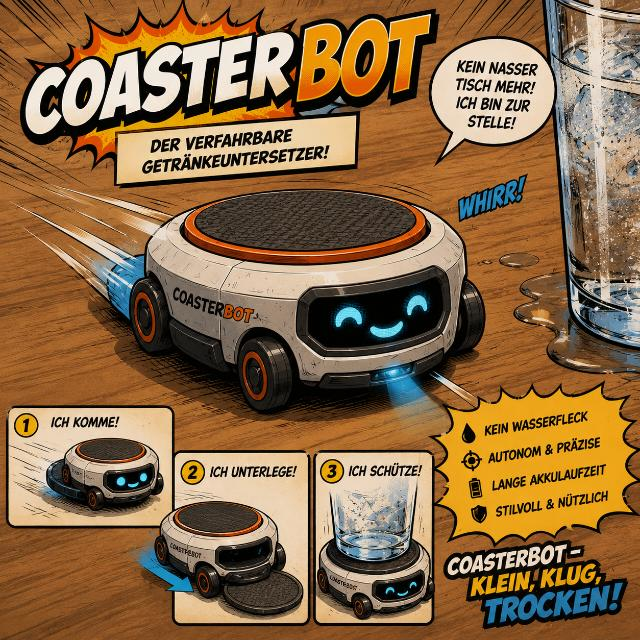
\includegraphics[width=0.38\textwidth]{coasterbot.png}} \\[1em]

\vspace{4em}

    {\normalsize
\begin{tabular}{ll}
Dennis Borutta, B. Eng & dennis.borutta@outlook.com\\
Stefan Etringer, B. Eng & mail@stefan.works\\
Gereon Such, M. Sc. & gereonsuch@gmail.com\\
\end{tabular}
    }
  \end{center}


\end{titlepage}


% einleitung preambel etc.


% Versionshistorie des Dokuments -- eigene Seite direkt nach dem Titelblatt
\section*{Versionshistorie}

\begin{tabularx}{\textwidth}{@{}clp{2.6cm}X@{}}
\toprule
\textbf{Version} & \textbf{Datum} & \textbf{Bearbeiter} & \textbf{Änderungen}\\
\midrule
1 & 09.08.2026 & Etringer & Erstfassung des Pflichtenhefts\\
2 & 10.08.2026 & Etringer & Anpassungen der Kapitelstruktur\\
3 & 10.08.2026 & Etringer & Strukturierung der Tabellen\\
\bottomrule
\end{tabularx}


\newpage

\tableofcontents

\newpage

\section{Einleitung}\label{einleitung}

\subsection{Zweck des Pflichtenhefts}\label{zweck-des-pflichtenhefts}

Dieses Pflichtenheft beschreibt die technische Umsetzung des im
Lastenheft definierten Coasterbot-Prototyps. Es dient als verbindliche
Grundlage für die Entwicklung der Systemarchitektur, der
Hardwarekomponenten, der Softwarekomponenten sowie der
Simulationsumgebung.

Während das Lastenheft die Anforderungen und Ziele des Auftraggebers
beschreibt, legt dieses Dokument die geplante Realisierung des Systems
fest. Es beschreibt die Architekturentscheidungen, die Aufteilung des
Systems in einzelne Komponenten sowie die vorgesehenen Verfahren zur
Umsetzung und Verifikation der geforderten Funktionen.

Das Pflichtenheft dient allen an der Entwicklung beteiligten Personen
als technische Referenz und ermöglicht eine nachvollziehbare Verbindung
zwischen Anforderungen, Implementierung und Tests.

\subsection{Projektbeschreibung}\label{projektbeschreibung}

Im Rahmen der Projektarbeit wird ein Prototyp eines autonomen mobilen
Roboters entwickelt, der als Coasterbot bezeichnet wird. Der Roboter
soll in gastronomischen Umgebungen eingesetzt werden und die Aufgabe
übernehmen, Getränkeuntersetzer selbstständig zu transportieren. Dieser
platziert die Untersetzer auf dem Tisch und nimmt sie erneut auf.

Der Fokus der Entwicklung liegt auf der Realisierung eines
funktionsfähigen Prototyps mit einer modularen Softwarearchitektur und
einer validierbaren Simulationsumgebung. Dabei werden insbesondere die
Bereiche autonome Navigation, Lokalisierung, Objekthandhabung,
Systemüberwachung und Sicherheit betrachtet.

Die Entwicklung erfolgt nach einem komponentenbasierten Ansatz, bei dem
Hardware- und Softwarekomponenten über definierte Schnittstellen
miteinander verbunden werden. Dadurch soll eine spätere Erweiterung des
Systems um zusätzliche Funktionen wie Bestellaufnahme, Reinigung oder
Getränketransport ermöglicht werden.

\subsection{Zielsetzung}\label{zielsetzung}

Ziel der technischen Umsetzung ist die Entwicklung eines prototypischen
Robotersystems, welches die im Lastenheft definierten Anforderungen des
Maturity Level 1 erfüllt.

Hierzu werden folgende Ergebnisse angestrebt:

\begin{itemize}
\tightlist
\item
  Entwicklung einer modularen Softwarearchitektur für die Steuerung des
  Roboters.
\item
  Entwicklung einer Hardwarearchitektur mit austauschbaren Sensor- und
  Aktorkomponenten.
\item
  Umsetzung einer Navigations- und Lokalisierungskomponente für den
  Betrieb auf einer Tischoberfläche.
\item
  Entwicklung einer Komponente zur Aufnahme, Positionierung und
  Wiederaufnahme von Getränkeuntersetzern.
\item
  Implementierung von Sicherheitsmechanismen zur Vermeidung von
  Kollisionen und Abstürzen.
\item
  Erstellung einer Simulationsumgebung zur Entwicklung und Validierung
  der Software.
\item
  Definition und Durchführung von Tests zur Überprüfung der
  Anforderungen.
\end{itemize}

Der Schwerpunkt liegt auf dem Nachweis der technischen Machbarkeit und
nicht auf der Entwicklung eines serienreifen Produkts.

\subsection{Technische
Zielarchitektur}\label{technische-zielarchitektur}

Der Coasterbot wird als eingebettetes, autonomes Robotersystem
umgesetzt. Die geplante Architektur besteht aus mehreren logisch
getrennten Ebenen:

\subsubsection{Hardwareebene}\label{hardwareebene}

Die Hardwareebene umfasst alle physischen Komponenten des Roboters:

\begin{itemize}
\tightlist
\item
  Recheneinheit zur Ausführung der Steuerungssoftware.
\item
  Sensorik zur Erfassung der Umgebung und des Systemzustands.
\item
  Aktorik zur Bewegung und Manipulation von Getränkeuntersetzern.
\item
  Energieversorgung, inklusive Akkumanagement.
\end{itemize}

\subsubsection{Abstraktionsebene}\label{abstraktionsebene}

Die Abstraktionsebene stellt eine einheitliche Schnittstelle zwischen
Hardware und Software bereit. Dadurch können konkrete
Hardwarekomponenten ausgetauscht werden, ohne die darüberliegenden
Softwarekomponenten anpassen zu müssen.

\subsubsection{Steuerungs- und
Anwendungsebene}\label{steuerungs--und-anwendungsebene}

Die Anwendungsebene beinhaltet die eigentliche Systemlogik:

\begin{itemize}
\tightlist
\item
  Navigation
\item
  Lokalisierung
\item
  Bewegungsplanung
\item
  Untersetzerhandling
\item
  Sicherheitslogik
\item
  Systemüberwachung
\end{itemize}

\subsubsection{Simulationsebene}\label{simulationsebene}

Die Simulationsebene ermöglicht die Ausführung und Validierung der
Software ohne physische Hardware. Dabei werden Sensoren, Aktoren und
Umgebungsbedingungen modelliert.

\subsection{Abgrenzung}\label{abgrenzung}

Die folgenden Funktionen werden im Rahmen dieser Projektarbeit nicht
umgesetzt:

\begin{itemize}
\tightlist
\item
  Automatisierter Getränketransport.
\item
  Automatisierte Tischreinigung.
\item
  Digitale Bestellaufnahme.
\item
  Integration von Bezahlsystemen.
\item
  Kommunikation über externe Netzwerke.
\item
  Kartierung und dauerhafte Speicherung der Umgebung.
\item
  Koordination mehrerer Coasterbots.
\item
  Steuerung von Komponenten über eine Nutzeroberfläche
\end{itemize}

Diese Funktionen werden ausschließlich als mögliche Erweiterungen
berücksichtigt und beeinflussen die Architektur nur hinsichtlich einer
zukünftigen Erweiterbarkeit.

\subsection{Dokumentstruktur}\label{dokumentstruktur}

Das Pflichtenheft ist wie folgt aufgebaut:

\textbf{Kapitel 1 -- Einleitung} Beschreibung der Zielsetzung,
Aufgabenstellung und Abgrenzung des Projekts.

\textbf{Kapitel 2 -- Systemarchitektur} Beschreibung der Gesamtstruktur
des Coasterbots sowie der Aufteilung in Hardware- und
Softwarekomponenten.

\textbf{Kapitel 3 -- Hardwarekonzept} Beschreibung der mechanischen
Komponenten, Sensorik, Aktorik und Energieversorgung.

\textbf{Kapitel 4 -- Softwarekonzept} Beschreibung der
Softwarearchitektur, Komponenten und Schnittstellen.

\textbf{Kapitel 5 -- Implementierungskonzept} Beschreibung der geplanten
Umsetzung der Kernfunktionen.

\textbf{Kapitel 6 -- Simulationskonzept} Beschreibung der
Simulationsumgebung und der modellierten Systembestandteile.

\textbf{Kapitel 7 -- Test- und Verifikationskonzept} Beschreibung der
Teststrategie und Zuordnung von Tests zu Anforderungen.

\textbf{Kapitel 8 -- Zusammenfassung und Ausblick} Bewertung der
Umsetzung sowie mögliche zukünftige Erweiterungen.

\section{Systemarchitektur}\label{systemarchitektur}

\subsection{Ziel der
Systemarchitektur}\label{ziel-der-systemarchitektur}

Die Systemarchitektur beschreibt den grundlegenden Aufbau des
Coasterbot-Prototyps sowie die Aufteilung des Gesamtsystems in einzelne
technische Komponenten. Ziel der Architektur ist es, eine robuste,
modulare und erweiterbare Struktur zu schaffen, welche die Umsetzung der
im Lastenheft definierten Anforderungen ermöglicht.

Die Architektur folgt einem komponentenbasierten Ansatz mit klar
definierten Schnittstellen zwischen den einzelnen Systembestandteilen.
Dadurch können einzelne Komponenten unabhängig voneinander entwickelt,
getestet und bei Bedarf ausgetauscht werden.

Besondere Bedeutung haben dabei die Trennung von Hardware und Software
sowie die Möglichkeit, das System vollständig oder teilweise in einer
Simulationsumgebung auszuführen.

\subsection{Systemaufbau}\label{systemaufbau}

Der Coasterbot wird als eingebettetes autonomes Robotersystem
entwickelt. Das Gesamtsystem wird in mehrere Ebenen unterteilt:

\begin{enumerate}
\def\labelenumi{\arabic{enumi}.}
\tightlist
\item
  Hardwareebene
\item
  Hardwareabstraktionsebene
\item
  Systemlogikebene
\item
  Anwendungsebene
\item
  Simulationsebene
\end{enumerate}

Die Ebenen sind hierarchisch aufgebaut und kommunizieren ausschließlich
über definierte Schnittstellen.

\subsection{Architekturmodell}\label{architekturmodell}

\subsubsection{Hardwareebene}\label{hardwareebene-1}

Die Hardwareebene bildet die physische Grundlage des Roboters. Sie
umfasst alle Komponenten, die zur Wahrnehmung der Umgebung, zur Bewegung
und zur Energieversorgung erforderlich sind.

Die Hardwareebene besteht aus folgenden Hauptkomponenten:

\begin{itemize}
\tightlist
\item
  Recheneinheit
\item
  Sensorik
\item
  Aktorik
\item
  Energieversorgung
\item
  Mechanische Konstruktion
\end{itemize}

Die Recheneinheit übernimmt die Verarbeitung der Sensordaten sowie die
Berechnung der Steuerbefehle für die Aktoren.

Die Sensorik stellt Informationen über den Zustand des Roboters und
seiner Umgebung bereit. Dazu gehören insbesondere:

\begin{itemize}
\tightlist
\item
  Erkennung von Hindernissen
\item
  Erkennung der Tischbegrenzung
\item
  Bestimmung der Position und Orientierung
\item
  Erkennung von Getränkeuntersetzern
\end{itemize}

Die Aktorik setzt die berechneten Steuerbefehle in physische Aktionen
um. Dazu gehören:

\begin{itemize}
\tightlist
\item
  Bewegung des Roboters
\item
  Aufnahme eines Getränkeuntersetzers
\item
  Positionierung eines Getränkeuntersetzers
\end{itemize}

\subsection{Hardwareabstraktionsebene}\label{hardwareabstraktionsebene}

Die Hardwareabstraktionsebene stellt eine Trennung zwischen der
physischen Hardware und der darüberliegenden Softwarelogik her.

Ziel dieser Ebene ist es, die Abhängigkeit der Software von konkreten
Hardwarekomponenten zu reduzieren. Dadurch können beispielsweise
unterschiedliche Sensoren oder Motoren verwendet werden, ohne die
Navigations- oder Steuerungslogik anzupassen.

Die Hardwareabstraktion umfasst:

\begin{itemize}
\tightlist
\item
  Einheitliche Schnittstellen für Sensoren
\item
  Einheitliche Schnittstellen für Aktoren
\item
  Verwaltung der Hardwarekommunikation
\item
  Umwandlung hardwareabhängiger Daten in ein einheitliches Format
\end{itemize}

Durch diese Struktur können reale Hardwarekomponenten durch
Simulationsmodelle ersetzt werden.

\subsection{Systemlogikebene}\label{systemlogikebene}

Die Systemlogikebene beinhaltet die zentralen Funktionen zur Steuerung
des Roboters. Sie verarbeitet Informationen aus der Hardwareabstraktion
und erzeugt entsprechende Steuerbefehle.

Die wesentlichen Komponenten dieser Ebene sind:

\subsubsection{Navigationskomponente}\label{navigationskomponente}

Die Navigationskomponente ist verantwortlich für die autonome Bewegung
des Roboters innerhalb des Arbeitsbereichs.

Aufgaben:

\begin{itemize}
\tightlist
\item
  Planung einer Fahrroute
\item
  Erkennung von Hindernissen
\item
  Anpassung der Route bei Änderungen der Umgebung
\item
  Erreichen definierter Zielpositionen
\end{itemize}

\subsubsection{Lokalisierungskomponente}\label{lokalisierungskomponente}

Die Lokalisierungskomponente bestimmt die aktuelle Position und
Orientierung des Roboters.

Aufgaben:

\begin{itemize}
\tightlist
\item
  Verarbeitung von Sensordaten
\item
  Positionsbestimmung
\item
  Aktualisierung der Roboterpose
\item
  Bereitstellung der Positionsinformationen für andere Komponenten
\end{itemize}

\subsubsection{Bewegungssteuerung}\label{bewegungssteuerung}

Die Bewegungssteuerung übersetzt Navigationsentscheidungen in konkrete
Bewegungsbefehle.

Aufgaben:

\begin{itemize}
\tightlist
\item
  Steuerung der Motoren
\item
  Geschwindigkeitsregelung
\item
  Begrenzung kritischer Bewegungszustände
\item
  Umsetzung von Sicherheitsanforderungen
\end{itemize}

\subsubsection{Untersetzerhandling}\label{untersetzerhandling}

Diese Komponente steuert die Aufnahme und Ausgabe von
Getränkeuntersetzern.

Aufgaben:

\begin{itemize}
\tightlist
\item
  Erkennen eines verfügbaren Untersetzers
\item
  Aktivieren des Aufnahmemechanismus
\item
  Transport des Untersetzers
\item
  Positionieren des Untersetzers
\item
  Überprüfung der erfolgreichen Ausgabe
\end{itemize}

\subsubsection{Sicherheitskomponente}\label{sicherheitskomponente}

Die Sicherheitskomponente überwacht sicherheitskritische Zustände.

Aufgaben:

\begin{itemize}
\tightlist
\item
  Erkennen gefährlicher Situationen
\item
  Auslösen eines kontrollierten Stopps
\item
  Überwachung sicherheitsrelevanter Sensoren
\item
  Wechsel in einen sicheren Zustand
\end{itemize}

\subsubsection{Systemüberwachung}\label{systemuxfcberwachung}

Die Systemüberwachung stellt Informationen über den Betriebszustand
bereit.

Aufgaben:

\begin{itemize}
\tightlist
\item
  Erkennung von Fehlern
\item
  Speicherung von Fehlerinformationen
\item
  Überwachung von Systemzuständen
\item
  Meldung fehlgeschlagener Aufgaben
\end{itemize}

\subsection{Anwendungsebene}\label{anwendungsebene}

Die Anwendungsebene beschreibt die übergeordnete Ablaufsteuerung des
Coasterbots.

Sie definiert die Reihenfolge der Systemaktionen und koordiniert die
einzelnen Funktionskomponenten.

Beispielhafter Ablauf:

\begin{enumerate}
\def\labelenumi{\arabic{enumi}.}
\tightlist
\item
  Initialisierung des Systems.
\item
  Überprüfung der Betriebsbereitschaft.
\item
  Erfassung der Umgebung.
\item
  Bestimmung eines Zielpunkts.
\item
  Planung einer Route.
\item
  Navigation zum Ziel.
\item
  Aufnahme oder Ausgabe eines Getränkeuntersetzers.
\item
  Überprüfung des Ergebnisses.
\item
  Rückmeldung über den Systemstatus.
\end{enumerate}

Die Anwendungsebene enthält keine hardwareabhängigen Funktionen und
kommuniziert ausschließlich über definierte Schnittstellen mit den
darunterliegenden Komponenten.

\subsection{Simulationsarchitektur}\label{simulationsarchitektur}

Die Simulation stellt eine parallele Umgebung zur realen Hardware dar.
Ziel ist es, die Softwarekomponenten unabhängig vom physischen Prototyp
entwickeln und testen zu können.

Die Simulationsarchitektur umfasst:

\subsubsection{Umgebungsmodell}\label{umgebungsmodell}

Das Umgebungsmodell beschreibt die virtuelle Tischoberfläche sowie
darauf befindliche Objekte.

Modelliert werden:

\begin{itemize}
\tightlist
\item
  Tischgrenzen
\item
  Hindernisse
\item
  Getränke
\item
  Getränkeuntersetzer
\end{itemize}

\subsubsection{Sensormodelle}\label{sensormodelle}

Sensormodelle erzeugen virtuelle Sensordaten entsprechend der
simulierten Umgebung.

Beispiele:

\begin{itemize}
\tightlist
\item
  Abstandswerte
\item
  Positionserkennung
\item
  Hinderniserkennung
\item
  Tischkantenerkennung
\end{itemize}

\subsubsection{Aktormodelle}\label{aktormodelle}

Aktormodelle bilden das Verhalten realer Aktoren nach.

Beispiele:

\begin{itemize}
\tightlist
\item
  Motorbewegungen
\item
  Geschwindigkeit
\item
  Aufnahme- und Ablegebewegungen
\end{itemize}

\subsubsection{Teststeuerung}\label{teststeuerung}

Die Teststeuerung ermöglicht die Durchführung reproduzierbarer
Testszenarien.

Sie ermöglicht:

\begin{itemize}
\tightlist
\item
  Start definierter Szenarien
\item
  Simulation von Fehlerzuständen
\item
  Vergleich erwarteter und tatsächlicher Ergebnisse
\end{itemize}

\subsection{Kommunikationsprinzipien}\label{kommunikationsprinzipien}

Die Kommunikation zwischen Komponenten erfolgt über klar definierte
Schnittstellen.

Folgende Prinzipien werden berücksichtigt:

\begin{itemize}
\tightlist
\item
  Komponenten besitzen eine eindeutige Verantwortlichkeit.
\item
  Direkte Abhängigkeiten zwischen nicht benachbarten Schichten werden
  vermieden.
\item
  Hardwareabhängige Implementierungen bleiben gekapselt.
\item
  Simulations- und Hardwarekomponenten verwenden identische
  Schnittstellen.
\item
  Datenformate werden einheitlich definiert.
\end{itemize}

\subsection{Erweiterbarkeit der
Architektur}\label{erweiterbarkeit-der-architektur}

Die Architektur wird so ausgelegt, dass zukünftige Entwicklungsstufen
integriert werden können.

Mögliche Erweiterungen:

\begin{itemize}
\tightlist
\item
  Bestellaufnahme
\item
  Bezahlung
\item
  Mensch-Roboter-Interaktion
\item
  Getränketransport
\item
  Automatische Reinigung
\item
  Kommunikation mehrerer Roboter
\end{itemize}

Die Erweiterungen sollen durch Ergänzung neuer Komponenten erfolgen
können, ohne die Kernfunktionen des Systems grundlegend zu verändern.

\subsection{Zusammenfassung}\label{zusammenfassung}

Die entwickelte Systemarchitektur bildet die Grundlage für die Umsetzung
des Coasterbot-Prototyps. Durch die Trennung in Hardware-,
Abstraktions-, Logik-, Anwendungs- und Simulationsebene wird eine
modulare und erweiterbare Struktur geschaffen.

Die Architektur ermöglicht eine unabhängige Entwicklung und Prüfung
einzelner Komponenten und erfüllt damit die im Lastenheft definierten
Anforderungen hinsichtlich Modularität, Testbarkeit und
Simulationsfähigkeit.

\section{Hardwarekonzept}\label{hardwarekonzept}

\subsection{Ziel des Hardwarekonzepts}\label{ziel-des-hardwarekonzepts}

Dieses Kapitel beschreibt die technische Auslegung der Hardware des
Coasterbot-Prototyps. Das Hardwarekonzept definiert die benötigten
Komponenten zur Realisierung der autonomen Navigation, der sicheren
Bewegung sowie der Aufnahme und Ausgabe von Getränkeuntersetzern.

Die Auswahl und Anordnung der Hardwarekomponenten erfolgt unter
Berücksichtigung der Anforderungen aus dem Lastenheft. Insbesondere
werden dabei die Anforderungen hinsichtlich Modularität,
Austauschbarkeit, Simulationsfähigkeit und Erweiterbarkeit
berücksichtigt.

Der Prototyp wird als kompakter, handtellergroßer mobiler Roboter
ausgelegt. Die Hardware muss daher eine geringe Baugröße, ein niedriges
Gewicht sowie einen energieeffizienten Betrieb ermöglichen.

\subsection{Hardwarearchitektur}\label{hardwarearchitektur}

Die Hardware des Coasterbots wird in folgende Hauptbereiche unterteilt:

\begin{itemize}
\tightlist
\item
  Recheneinheit
\item
  Sensorik
\item
  Aktorik
\item
  Energieversorgung
\item
  Kommunikationsschnittstellen
\item
  Mechanische Konstruktion
\end{itemize}

Die einzelnen Komponenten werden modular aufgebaut und über definierte
Schnittstellen miteinander verbunden.

\subsection{Recheneinheit}\label{recheneinheit}

Die Recheneinheit bildet die zentrale Verarbeitungseinheit des Roboters.
Sie übernimmt die Verarbeitung der Sensordaten, die Ausführung der
Steuerungssoftware sowie die Berechnung der Bewegungsbefehle.

Die Anforderungen an die Recheneinheit sind:

\begin{longtable}[]{@{}
  >{\raggedright\arraybackslash}p{(\linewidth - 2\tabcolsep) * \real{0.1788}}
  >{\raggedright\arraybackslash}p{(\linewidth - 2\tabcolsep) * \real{0.8212}}@{}}
\toprule\noalign{}
\begin{minipage}[b]{\linewidth}\raggedright
ID
\end{minipage} & \begin{minipage}[b]{\linewidth}\raggedright
Anforderung
\end{minipage} \\
\midrule\noalign{}
\endhead
\bottomrule\noalign{}
\endlastfoot
HW-CPU-001 & Die Recheneinheit muss ausreichend Rechenleistung für die
Verarbeitung von Sensordaten und Steueralgorithmen bereitstellen. \\
HW-CPU-002 & Die Recheneinheit muss die Ausführung der modularen
Softwarearchitektur ermöglichen. \\
HW-CPU-003 & Die Recheneinheit muss eine Kommunikation mit Sensoren und
Aktoren ermöglichen. \\
HW-CPU-004 & Die Recheneinheit muss eine Ausführung der Software in der
Simulationsumgebung unterstützen. \\
\end{longtable}

Für den Prototyp wird eine Trennung zwischen leistungsintensiver
Verarbeitung und hardwarenaher Steuerung vorgesehen. Dadurch können
zeitkritische Aufgaben wie Motorregelung oder Sensorauswertung
unabhängig von komplexeren Berechnungen ausgeführt werden.

\subsection{Sensorik}\label{sensorik}

Die Sensorik ermöglicht die Wahrnehmung der Umgebung sowie die Erfassung
des Systemzustands. Die Auswahl der Sensoren orientiert sich an den
Anforderungen der Navigation, Sicherheit und Objektbehandlung.

\subsubsection{Hinderniserkennung}\label{hinderniserkennung}

Zur sicheren Navigation muss der Coasterbot Hindernisse innerhalb seines
Arbeitsbereichs erkennen können.

Die Sensorik muss folgende Anforderungen erfüllen:

\begin{longtable}[]{@{}
  >{\raggedright\arraybackslash}p{(\linewidth - 2\tabcolsep) * \real{0.1759}}
  >{\raggedright\arraybackslash}p{(\linewidth - 2\tabcolsep) * \real{0.8241}}@{}}
\toprule\noalign{}
\begin{minipage}[b]{\linewidth}\raggedright
ID
\end{minipage} & \begin{minipage}[b]{\linewidth}\raggedright
Anforderung
\end{minipage} \\
\midrule\noalign{}
\endhead
\bottomrule\noalign{}
\endlastfoot
HW-SEN-001 & Die Sensorik muss Objekte im Fahrbereich erkennen
können. \\
HW-SEN-002 & Die Sensorik muss Informationen zur Kollisionsvermeidung
bereitstellen. \\
HW-SEN-003 & Die erfassten Sensordaten müssen von der
Navigationskomponente verarbeitet werden können. \\
\end{longtable}

Mögliche technische Lösungen sind Abstandssensoren, Kameras oder
Kombinationen verschiedener Sensorprinzipien.

\subsubsection{Tischkantenerkennung}\label{tischkantenerkennung}

Da der Roboter ausschließlich auf einer Tischoberfläche betrieben wird,
ist eine zuverlässige Erkennung der Tischbegrenzung erforderlich.

Anforderungen:

\begin{longtable}[]{@{}
  >{\raggedright\arraybackslash}p{(\linewidth - 2\tabcolsep) * \real{0.1863}}
  >{\raggedright\arraybackslash}p{(\linewidth - 2\tabcolsep) * \real{0.8137}}@{}}
\toprule\noalign{}
\begin{minipage}[b]{\linewidth}\raggedright
ID
\end{minipage} & \begin{minipage}[b]{\linewidth}\raggedright
Anforderung
\end{minipage} \\
\midrule\noalign{}
\endhead
\bottomrule\noalign{}
\endlastfoot
HW-SEN-004 & Sensoren müssen die Annäherung an eine Tischkante erkennen
können. \\
HW-SEN-005 & Die Tischkantenerkennung muss eine rechtzeitige Reaktion
der Steuerung ermöglichen. \\
\end{longtable}

Die Erkennung der Tischkante stellt eine zentrale Sicherheitsfunktion
dar und wird unabhängig von der normalen Hinderniserkennung betrachtet.

\subsubsection{Positions- und
Orientierungserfassung}\label{positions--und-orientierungserfassung}

Für die autonome Navigation benötigt der Roboter Informationen über
seine Position und Orientierung.

Anforderungen:

\begin{longtable}[]{@{}
  >{\raggedright\arraybackslash}p{(\linewidth - 2\tabcolsep) * \real{0.1648}}
  >{\raggedright\arraybackslash}p{(\linewidth - 2\tabcolsep) * \real{0.8352}}@{}}
\toprule\noalign{}
\begin{minipage}[b]{\linewidth}\raggedright
ID
\end{minipage} & \begin{minipage}[b]{\linewidth}\raggedright
Anforderung
\end{minipage} \\
\midrule\noalign{}
\endhead
\bottomrule\noalign{}
\endlastfoot
HW-SEN-006 & Das System muss Informationen zur Positionsbestimmung
bereitstellen. \\
HW-SEN-007 & Das System muss Informationen zur Bestimmung der
Orientierung bereitstellen. \\
\end{longtable}

Die Positionsbestimmung kann durch eine Kombination verschiedener
Sensorquellen erfolgen.

\subsection{Aktorik}\label{aktorik}

Die Aktorik setzt die berechneten Steuerbefehle in physische Aktionen
um.

Die Aktorik wird in zwei Bereiche unterteilt:

\begin{itemize}
\tightlist
\item
  Bewegungsaktorik
\item
  Manipulationsaktorik
\end{itemize}

\subsection{Bewegungsaktorik}\label{bewegungsaktorik}

Die Bewegungsaktorik ermöglicht die autonome Fortbewegung des
Coasterbots auf der Tischoberfläche.

Anforderungen:

\begin{longtable}[]{@{}
  >{\raggedright\arraybackslash}p{(\linewidth - 2\tabcolsep) * \real{0.1149}}
  >{\raggedright\arraybackslash}p{(\linewidth - 2\tabcolsep) * \real{0.8851}}@{}}
\toprule\noalign{}
\begin{minipage}[b]{\linewidth}\raggedright
ID
\end{minipage} & \begin{minipage}[b]{\linewidth}\raggedright
Anforderung
\end{minipage} \\
\midrule\noalign{}
\endhead
\bottomrule\noalign{}
\endlastfoot
HW-ACT-001 & Der Roboter muss sich kontrolliert in verschiedene
Richtungen bewegen können. \\
HW-ACT-002 & Die Geschwindigkeit muss steuerbar sein. \\
HW-ACT-003 & Die Bewegung muss durch die Software geregelt werden
können. \\
HW-ACT-004 & Die Bewegung muss für die Simulation abstrahiert werden
können. \\
\end{longtable}

Für den Prototyp wird ein Antriebssystem vorgesehen, das eine präzise
Steuerung der Fahrbewegung ermöglicht.

\subsection{Manipulationsaktorik}\label{manipulationsaktorik}

Die Manipulationsaktorik ermöglicht die Aufnahme und Ausgabe von
Getränkeuntersetzern.

Anforderungen:

\begin{longtable}[]{@{}
  >{\raggedright\arraybackslash}p{(\linewidth - 2\tabcolsep) * \real{0.1765}}
  >{\raggedright\arraybackslash}p{(\linewidth - 2\tabcolsep) * \real{0.8235}}@{}}
\toprule\noalign{}
\begin{minipage}[b]{\linewidth}\raggedright
ID
\end{minipage} & \begin{minipage}[b]{\linewidth}\raggedright
Anforderung
\end{minipage} \\
\midrule\noalign{}
\endhead
\bottomrule\noalign{}
\endlastfoot
HW-ACT-005 & Der Aufnahmemechanismus muss einen Getränkeuntersetzer
greifen können. \\
HW-ACT-006 & Der Mechanismus muss eine kontrollierte Positionierung
ermöglichen. \\
HW-ACT-007 & Der Zustand des Aufnahmevorgangs muss überprüfbar sein. \\
\end{longtable}

Der Mechanismus muss so ausgelegt werden, dass Getränkeuntersetzer
sicher bewegt werden können, ohne diese oder andere Gegenstände auf dem
Tisch zu beschädigen.

\subsection{Energieversorgung}\label{energieversorgung}

Die Energieversorgung stellt die elektrische Versorgung aller
Systemkomponenten sicher.

Sie umfasst:

\begin{itemize}
\tightlist
\item
  Energiespeicher
\item
  Spannungsregelung
\item
  Ladeelektronik
\item
  Überwachung des Energiezustands
\end{itemize}

Anforderungen:

\begin{longtable}[]{@{}
  >{\raggedright\arraybackslash}p{(\linewidth - 2\tabcolsep) * \real{0.1759}}
  >{\raggedright\arraybackslash}p{(\linewidth - 2\tabcolsep) * \real{0.8241}}@{}}
\toprule\noalign{}
\begin{minipage}[b]{\linewidth}\raggedright
ID
\end{minipage} & \begin{minipage}[b]{\linewidth}\raggedright
Anforderung
\end{minipage} \\
\midrule\noalign{}
\endhead
\bottomrule\noalign{}
\endlastfoot
HW-PWR-001 & Die Energieversorgung muss alle Hardwarekomponenten mit
ausreichender Leistung versorgen. \\
HW-PWR-002 & Der Akkuzustand muss überwacht werden können. \\
HW-PWR-003 & Das System muss bei unzureichender Energieversorgung
kontrolliert beendet werden können. \\
HW-PWR-004 & Die Energieversorgung muss austauschbar aufgebaut sein. \\
\end{longtable}

Die Energieversorgung wird so ausgelegt, dass ein ausreichender
Betriebszeitraum für Tests und Demonstrationen ermöglicht wird.

\subsection{Mechanische Konstruktion}\label{mechanische-konstruktion}

Die mechanische Konstruktion bildet die physische Struktur des
Coasterbots.

Anforderungen:

\begin{longtable}[]{@{}
  >{\raggedright\arraybackslash}p{(\linewidth - 2\tabcolsep) * \real{0.1827}}
  >{\raggedright\arraybackslash}p{(\linewidth - 2\tabcolsep) * \real{0.8173}}@{}}
\toprule\noalign{}
\begin{minipage}[b]{\linewidth}\raggedright
ID
\end{minipage} & \begin{minipage}[b]{\linewidth}\raggedright
Anforderung
\end{minipage} \\
\midrule\noalign{}
\endhead
\bottomrule\noalign{}
\endlastfoot
HW-MEC-001 & Die Konstruktion muss die Integration aller
Hardwarekomponenten ermöglichen. \\
HW-MEC-002 & Die Abmessungen müssen den Anforderungen eines
handtellergroßen Roboters entsprechen. \\
HW-MEC-003 & Die Konstruktion muss ausreichend stabil für den
vorgesehenen Betrieb sein. \\
HW-MEC-004 & Die Konstruktion muss als digitale CAD-Datei dokumentiert
werden. \\
HW-MEC-005 & Fertigungsrelevante Bauteile müssen als STL-Dateien
bereitgestellt werden. \\
\end{longtable}

Bei der Konstruktion werden insbesondere folgende Eigenschaften
berücksichtigt:

\begin{itemize}
\tightlist
\item
  geringes Gewicht,
\item
  einfache Fertigung,
\item
  Wartbarkeit,
\item
  Austauschbarkeit einzelner Komponenten,
\item
  Erweiterbarkeit für zukünftige Funktionen.
\end{itemize}

\subsection{Bedienelemente}\label{bedienelemente}

Für die direkte Bedienung durch das Servicepersonal oder Gäste besitzt
der Coasterbot einige wenige physische Bedienelemente.

Vorgesehen sind drei Bedienelemente:

\begin{itemize}
\tightlist
\item
  \textbf{Ein/Aus-Schalter:} Schaltet die Energieversorgung und damit
  das Gesamtsystem ein und aus. Er löst den Übergang zwischen den
  Zuständen \emph{AUS} und \emph{Initialisierung} bzw.
  \emph{Bereitschaft} aus.
\item
  \textbf{Aktionsknopf (Untersetzer-Ereignis):} Zentraler
  Multifunktionsknopf zum Auslösen eines Untersetzer-Vorgangs ohne
  weitere Eingabegeräte. Als plausibles Bedienschema ist vorgesehen: ein
  kurzer Tastendruck löst die Ausgabe eines Getränkeuntersetzers aus,
  ein längeres Halten (ca. zwei Sekunden) startet das Einsammeln bereits
  ausgelegter Untersetzer bzw. bricht einen laufenden Vorgang ab.
\item
  \textbf{Not-Aus-Taster:} Überführt den Roboter unmittelbar in einen
  sicheren Zustand und erfüllt damit die Anforderung SAF-005 aus dem
  Lastenheft.
\end{itemize}

Die Anforderungen an die Bedienelemente sind:

\begin{longtable}[]{@{}
  >{\raggedright\arraybackslash}p{(\linewidth - 2\tabcolsep) * \real{0.1242}}
  >{\raggedright\arraybackslash}p{(\linewidth - 2\tabcolsep) * \real{0.8758}}@{}}
\toprule\noalign{}
\begin{minipage}[b]{\linewidth}\raggedright
ID
\end{minipage} & \begin{minipage}[b]{\linewidth}\raggedright
Anforderung
\end{minipage} \\
\midrule\noalign{}
\endhead
\bottomrule\noalign{}
\endlastfoot
HW-BTN-001 & Ein Ein/Aus-Schalter muss das System kontrolliert ein- und
ausschalten können. \\
HW-BTN-002 & Ein zentraler Aktionsknopf muss Untersetzer-Ereignisse
auslösen können und dabei zwischen kurzem und langem Tastendruck
unterscheiden. \\
HW-BTN-003 & Ein Not-Aus-Taster muss den Roboter jederzeit in einen
sicheren Zustand überführen können (siehe SAF-005). \\
\end{longtable}

Die Bedienelemente werden über die Hardwareabstraktionsschicht als
Ereignisse an die Anwendungs- bzw. Sicherheitslogik weitergereicht und
können in der Simulation über dieselbe Schnittstelle nachgebildet
werden.

\subsection{Hardwareabstraktion}\label{hardwareabstraktion}

Alle Hardwarekomponenten werden so integriert, dass sie über definierte
Schnittstellen angesprochen werden können.

Die Hardwareabstraktion ermöglicht:

\begin{itemize}
\tightlist
\item
  Austausch einzelner Sensoren,
\item
  Austausch einzelner Aktoren,
\item
  Verwendung identischer Schnittstellen in der Simulation,
\item
  unabhängige Entwicklung von Hard- und Software.
\end{itemize}

Dadurch wird sichergestellt, dass Änderungen an der Hardware keine
grundlegenden Anpassungen der Systemlogik erfordern.

\subsection{Zusammenfassung}\label{zusammenfassung-1}

Das Hardwarekonzept definiert die technische Grundlage des
Coasterbot-Prototyps. Durch die modulare Struktur können Sensorik,
Aktorik und Energieversorgung unabhängig voneinander entwickelt und
erweitert werden.

Die Hardwarearchitektur unterstützt damit die zentralen
Entwicklungsziele des Projekts:

\begin{itemize}
\tightlist
\item
  autonome Navigation,
\item
  sichere Bewegung,
\item
  automatisierte Handhabung von Getränkeuntersetzern,
\item
  Simulation und Testbarkeit,
\item
  Erweiterbarkeit zukünftiger Systemfunktionen.
\end{itemize}

\section{Softwarekonzept}\label{softwarekonzept}

\subsection{Ziel des Softwarekonzepts}\label{ziel-des-softwarekonzepts}

Dieses Kapitel beschreibt die technische Umsetzung der
Softwarearchitektur des Coasterbot-Prototyps. Das Softwarekonzept
definiert die Struktur der Softwarekomponenten, deren
Verantwortlichkeiten sowie die Kommunikationsschnittstellen zwischen den
einzelnen Modulen.

Die Software wird entsprechend den Anforderungen des Lastenhefts
komponentenbasiert, modular und hardwareunabhängig entwickelt. Dadurch
wird ermöglicht, einzelne Funktionen unabhängig voneinander zu
entwickeln, zu testen und bei zukünftigen Erweiterungen
wiederzuverwenden.

Ein zentraler Bestandteil des Softwarekonzepts ist die Trennung zwischen
hardwareabhängigen Funktionen und der eigentlichen Systemlogik. Dadurch
kann die Software sowohl auf der realen Hardware als auch innerhalb der
Simulationsumgebung ausgeführt werden.

\subsection{Softwarearchitektur}\label{softwarearchitektur}

Die Softwarearchitektur orientiert sich an einem geschichteten
Architekturmodell. Die einzelnen Schichten besitzen klar definierte
Aufgaben und kommunizieren ausschließlich über festgelegte
Schnittstellen.

Die Software wird in folgende Ebenen unterteilt:

\begin{enumerate}
\def\labelenumi{\arabic{enumi}.}
\tightlist
\item
  Hardwaretreiberebene
\item
  Hardwareabstraktionsebene
\item
  Systemdienste
\item
  Funktionskomponenten
\item
  Anwendungsebene
\end{enumerate}

\subsection{Hardwaretreiberebene}\label{hardwaretreiberebene}

Die Hardwaretreiberebene stellt die direkte Verbindung zwischen Software
und physischer Hardware her.

Sie beinhaltet hardwarespezifische Implementierungen für:

\begin{itemize}
\tightlist
\item
  Sensoransteuerung,
\item
  Motorsteuerung,
\item
  Manipulationsmechanismen,
\item
  Energieüberwachung,
\item
  Kommunikationsschnittstellen.
\end{itemize}

Die Aufgaben dieser Ebene sind:

\begin{itemize}
\tightlist
\item
  Initialisierung der Hardwarekomponenten.
\item
  Verarbeitung hardwareabhängiger Kommunikationsprotokolle.
\item
  Bereitstellung von Rohdaten für höhere Softwareebenen.
\item
  Umsetzung von Steuerbefehlen in Hardwareaktionen.
\end{itemize}

Die Hardwaretreiberebene wird so gestaltet, dass Änderungen an der
verwendeten Hardware möglichst keine Auswirkungen auf die
darüberliegenden Softwarekomponenten haben.

\subsection{Hardwareabstraktionsebene}\label{hardwareabstraktionsebene-1}

Die Hardwareabstraktionsebene bildet die Schnittstelle zwischen Hardware
und Systemlogik.

Ziel dieser Ebene ist die Bereitstellung einheitlicher Schnittstellen
unabhängig von der konkreten Hardwareimplementierung.

Beispiele:

\begin{longtable}[]{@{}ll@{}}
\toprule\noalign{}
Hardwarefunktion & Abstrakte Schnittstelle \\
\midrule\noalign{}
\endhead
\bottomrule\noalign{}
\endlastfoot
Abstandssensor & Entfernungsmessung \\
Motor & Geschwindigkeits- und Richtungssteuerung \\
Greifmechanismus & Aufnahme- und Ablagefunktion \\
Batteriesensor & Energiezustand \\
\end{longtable}

Die Hardwareabstraktion ermöglicht:

\begin{itemize}
\tightlist
\item
  Austausch von Sensoren und Aktoren.
\item
  Wiederverwendung der Software in der Simulation.
\item
  Vereinfachte Tests einzelner Komponenten.
\item
  Entkopplung von Hardware und Anwendungslogik.
\end{itemize}

\subsection{Systemdienste}\label{systemdienste}

Die Systemdienste stellen grundlegende Funktionen bereit, die von
mehreren Komponenten verwendet werden.

\subsubsection{Kommunikationsdienst}\label{kommunikationsdienst}

Der Kommunikationsdienst übernimmt den Austausch von Daten zwischen
Softwarekomponenten.

Aufgaben:

\begin{itemize}
\tightlist
\item
  Übertragung von Zustandsinformationen.
\item
  Weiterleitung von Steuerbefehlen.
\item
  Verwaltung definierter Kommunikationsschnittstellen.
\end{itemize}

\subsubsection{Konfigurationsdienst}\label{konfigurationsdienst}

Der Konfigurationsdienst verwaltet systemrelevante Parameter.

Beispiele:

\begin{itemize}
\tightlist
\item
  Sensorkonfiguration.
\item
  Fahrparameter.
\item
  Sicherheitsgrenzen.
\item
  Simulationsparameter.
\end{itemize}

Durch die zentrale Verwaltung können Parameter angepasst werden, ohne
die Softwarestruktur verändern zu müssen.

\subsubsection{Diagnosedienst}\label{diagnosedienst}

Der Diagnosedienst überwacht den Systemzustand und stellt Informationen
für Fehleranalyse und Wartung bereit.

Aufgaben:

\begin{itemize}
\tightlist
\item
  Erkennung von Fehlerzuständen.
\item
  Speicherung von Diagnoseinformationen.
\item
  Bereitstellung von Statusinformationen.
\end{itemize}

\subsection{Funktionskomponenten}\label{funktionskomponenten}

Die Funktionskomponenten enthalten die eigentliche Systemlogik des
Coasterbots.

\subsection{Navigationskomponente}\label{navigationskomponente-1}

Die Navigationskomponente ist für die autonome Bewegung des Roboters
verantwortlich.

Aufgaben:

\begin{itemize}
\tightlist
\item
  Verarbeitung von Umgebungsinformationen.
\item
  Planung einer Fahrroute.
\item
  Erkennung von Hindernissen.
\item
  Anpassung der Route bei Veränderungen.
\item
  Erreichen definierter Zielpositionen.
\end{itemize}

Die Navigationskomponente erhält Informationen über:

\begin{itemize}
\tightlist
\item
  aktuelle Position,
\item
  Orientierung,
\item
  Hindernisse,
\item
  Zielposition.
\end{itemize}

Als Ergebnis erzeugt sie Bewegungsbefehle für die Bewegungssteuerung.

\subsection{Lokalisierungskomponente}\label{lokalisierungskomponente-1}

Die Lokalisierungskomponente bestimmt die aktuelle Position und
Orientierung des Roboters.

Aufgaben:

\begin{itemize}
\tightlist
\item
  Verarbeitung von Sensordaten.
\item
  Berechnung der Roboterposition.
\item
  Aktualisierung der aktuellen Pose.
\item
  Bereitstellung der Positionsdaten für Navigation und Steuerung.
\end{itemize}

Die Lokalisierung ist notwendig, damit der Roboter definierte Zielpunkte
zuverlässig erreichen kann.

\subsection{Bewegungssteuerung}\label{bewegungssteuerung-1}

Die Bewegungssteuerung übersetzt Navigationsbefehle in konkrete
Aktorbefehle.

Aufgaben:

\begin{itemize}
\tightlist
\item
  Steuerung der Antriebsmotoren.
\item
  Regelung von Geschwindigkeit und Richtung.
\item
  Begrenzung sicherheitskritischer Bewegungen.
\item
  Umsetzung von Stoppsignalen.
\end{itemize}

Die Bewegungssteuerung stellt sicher, dass Bewegungen kontrolliert und
reproduzierbar erfolgen.

\subsection{Untersetzerhandling}\label{untersetzerhandling-1}

Die Komponente für das Untersetzerhandling steuert alle Funktionen zur
Aufnahme und Ausgabe von Getränkeuntersetzern.

Aufgaben:

\begin{itemize}
\tightlist
\item
  Erkennen eines Untersetzers.
\item
  Aktivieren des Aufnahmemechanismus.
\item
  Transport des Untersetzers.
\item
  Positionierung unter einem Getränk.
\item
  Überprüfung der erfolgreichen Platzierung.
\item
  Aufnahme eines gebrauchten Untersetzers.
\end{itemize}

Die Komponente arbeitet mit der Navigation und Sensorik zusammen, um
eine präzise Positionierung zu ermöglichen.

\subsection{Sicherheitskomponente}\label{sicherheitskomponente-1}

Die Sicherheitskomponente überwacht alle sicherheitsrelevanten Zustände.

Aufgaben:

\begin{itemize}
\tightlist
\item
  Überwachung kritischer Sensorwerte.
\item
  Erkennung von Gefahrensituationen.
\item
  Auslösen eines Notstopps.
\item
  Wechsel in einen sicheren Zustand.
\end{itemize}

Die Sicherheitslogik besitzt eine hohe Priorität gegenüber anderen
Systemfunktionen.

Beispiele:

\begin{itemize}
\tightlist
\item
  Erkennen einer Tischkante.
\item
  Verlust eines relevanten Sensorsignals.
\item
  Annäherung an ein Hindernis.
\item
  Fehlfunktion eines Aktors.
\end{itemize}

\subsection{Systemüberwachung}\label{systemuxfcberwachung-1}

Die Systemüberwachung stellt Informationen über den Betriebszustand
bereit.

Aufgaben:

\begin{itemize}
\tightlist
\item
  Überwachung der Komponenten.
\item
  Erkennung von Fehlern.
\item
  Protokollierung von Ereignissen.
\item
  Anzeige des aktuellen Systemstatus.
\item
  Erkennung erfolgreicher oder fehlgeschlagener Aufgaben.
\end{itemize}

\subsection{Zustandsmodell des
Coasterbots}\label{zustandsmodell-des-coasterbots}

Die Ablaufsteuerung des Systems wird durch ein Zustandsmodell umgesetzt.

Der Coasterbot besitzt folgende Hauptzustände:

\begin{longtable}[]{@{}ll@{}}
\toprule\noalign{}
Zustand & Beschreibung \\
\midrule\noalign{}
\endhead
\bottomrule\noalign{}
\endlastfoot
Initialisierung & Start und Überprüfung der Systemkomponenten \\
Bereitschaft & System ist einsatzbereit \\
Navigation & Roboter bewegt sich zu einem Zielpunkt \\
Untersetzeraufnahme & Aufnahme eines Getränkeuntersetzers \\
Untersetzerplatzierung & Positionierung des Untersetzers \\
Aufgabe abgeschlossen & Erfolgreicher Abschluss einer Aktion \\
Fehlerzustand & Systemfehler erkannt \\
Sicherheitsstopp & Sofortiger Halt aufgrund einer Gefahr \\
\end{longtable}

Der Wechsel zwischen Zuständen erfolgt ausschließlich durch definierte
Ereignisse und Bedingungen.

\subsection{Fehlerbehandlung}\label{fehlerbehandlung}

Die Software muss Fehlerzustände kontrolliert behandeln.

Folgende Fehlerfälle werden berücksichtigt:

\begin{itemize}
\tightlist
\item
  Sensorausfall.
\item
  Kommunikationsfehler zwischen Komponenten.
\item
  Blockierung eines Aktors.
\item
  Verlust der Lokalisierung.
\item
  Kritischer Energiezustand.
\end{itemize}

Bei einem Fehler führt das System abhängig von der Fehlerart eine
geeignete Reaktion aus:

\begin{itemize}
\tightlist
\item
  Wiederholung einer Aktion.
\item
  Wechsel in einen sicheren Zustand.
\item
  Abbruch einer Aufgabe.
\item
  Ausgabe einer Fehlermeldung.
\end{itemize}

\subsection{Schnittstellenkonzept}\label{schnittstellenkonzept}

Die Softwarekomponenten kommunizieren über klar definierte
Schnittstellen.

Beispiele:

\begin{longtable}[]{@{}lll@{}}
\toprule\noalign{}
Schnittstelle & Quelle & Ziel \\
\midrule\noalign{}
\endhead
\bottomrule\noalign{}
\endlastfoot
Sensordaten & Hardwareabstraktion & Navigation \\
Positionsdaten & Lokalisierung & Navigation \\
Bewegungsbefehle & Navigation & Bewegungssteuerung \\
Statusinformationen & Systemkomponenten & Systemüberwachung \\
Simulationsdaten & Simulationsumgebung & Hardwareabstraktion \\
\end{longtable}

Die Schnittstellen werden so gestaltet, dass einzelne Komponenten
unabhängig ausgetauscht werden können.

\subsection{Zusammenfassung}\label{zusammenfassung-2}

Das Softwarekonzept definiert eine modulare und erweiterbare Architektur
für den Coasterbot-Prototyp. Durch die Trennung von Hardware,
Abstraktion und Systemlogik wird eine flexible Entwicklungsumgebung
geschaffen.

Die Architektur ermöglicht:

\begin{itemize}
\tightlist
\item
  unabhängige Entwicklung einzelner Komponenten,
\item
  automatisierte Tests,
\item
  Nutzung einer Simulationsumgebung,
\item
  Austausch von Hardwarekomponenten,
\item
  Erweiterung um zukünftige Funktionen.
\end{itemize}

Damit erfüllt das Softwarekonzept die im Lastenheft definierten
Anforderungen hinsichtlich Modularität, Testbarkeit und Erweiterbarkeit.

\section{Implementierungskonzept}\label{implementierungskonzept}

\subsection{Ziel des
Implementierungskonzepts}\label{ziel-des-implementierungskonzepts}

Dieses Kapitel beschreibt die geplante technische Umsetzung der im
Softwarekonzept definierten Architektur. Das Implementierungskonzept
legt fest, wie die einzelnen Softwarekomponenten realisiert werden und
welche Methoden, Schnittstellen und Entwicklungsprinzipien dabei
eingesetzt werden.

Die Implementierung erfolgt mit dem Ziel, einen wartbaren, modularen und
testbaren Softwareprototypen für den Coasterbot zu entwickeln. Dabei
wird besonders berücksichtigt, dass die Software sowohl auf der realen
Hardware als auch in der Simulationsumgebung eingesetzt werden kann.

Die Umsetzung orientiert sich an den Anforderungen des Lastenhefts
hinsichtlich:

\begin{itemize}
\tightlist
\item
  Modularität,
\item
  Hardwareabstraktion,
\item
  Erweiterbarkeit,
\item
  automatisierter Testbarkeit,
\item
  Simulationsfähigkeit.
\end{itemize}

\subsection{Entwicklungsumgebung}\label{entwicklungsumgebung}

Die Entwicklung der Software erfolgt in einer Umgebung, die eine
strukturierte Entwicklung und Validierung der einzelnen Komponenten
ermöglicht.

Die Entwicklungsumgebung umfasst:

\begin{itemize}
\tightlist
\item
  Versionsverwaltung zur Nachverfolgung von Änderungen.
\item
  Entwicklungsumgebung zur Bearbeitung und Analyse des Quellcodes.
\item
  Build-System zur automatisierten Erstellung ausführbarer Software.
\item
  Testumgebung zur Durchführung automatisierter Tests.
\item
  Simulationsumgebung zur Validierung des Systemverhaltens.
\end{itemize}

Die verwendeten Werkzeuge und Frameworks werden so ausgewählt, dass sie
eine komponentenbasierte Entwicklung unterstützen.

\subsection{Programmiersprache und
Softwarestruktur}\label{programmiersprache-und-softwarestruktur}

Die Software wird objektorientiert und modular entwickelt. Die Wahl der
Programmiersprache erfolgt anhand folgender Kriterien:

\begin{itemize}
\tightlist
\item
  Unterstützung objektorientierter Programmierung.
\item
  Verfügbarkeit geeigneter Bibliotheken für Robotik und Simulation.
\item
  Unterstützung automatisierter Tests.
\item
  Gute Wartbarkeit und Erweiterbarkeit.
\end{itemize}

Die Softwarestruktur wird nach Verantwortlichkeiten getrennt aufgebaut.

Eine mögliche Projektstruktur ist:

\begin{verbatim}
Coasterbot
│
├── hardware
│   ├── sensors
│   ├── actuators
│   └── communication
│
├── abstraction
│   ├── sensor_interfaces
│   ├── actuator_interfaces
│   └── hardware_models
│
├── navigation
│   ├── localization
│   ├── path_planning
│   └── obstacle_avoidance
│
├── manipulation
│   └── coaster_handling
│
├── safety
│   └── safety_controller
│
├── monitoring
│   └── diagnostics
│
├── simulation
│   ├── environment
│   ├── sensors
│   └── actuators
│
└── tests
    ├── unit_tests
    └── integration_tests
\end{verbatim}

Diese Struktur ermöglicht eine klare Trennung der einzelnen
Verantwortlichkeiten.

\subsection{Umsetzung der
Hardwareabstraktion}\label{umsetzung-der-hardwareabstraktion}

Die Hardwareabstraktion wird über Schnittstellen umgesetzt. Jede
Hardwarekomponente erhält eine standardisierte Softwarebeschreibung.

Beispiel:

Ein Abstandssensor wird nicht direkt durch die Navigationslogik
angesprochen. Stattdessen stellt die Hardwareabstraktion eine allgemeine
Schnittstelle bereit:

\begin{verbatim}
DistanceSensor
|
├── RealDistanceSensor
|
└── SimulationDistanceSensor
\end{verbatim}

Dadurch kann die gleiche Navigationssoftware sowohl mit realen
Sensordaten als auch mit simulierten Daten betrieben werden.

Die Vorteile dieser Struktur sind:

\begin{itemize}
\tightlist
\item
  Austauschbarkeit von Hardware.
\item
  Vereinfachte Tests.
\item
  Reduzierung von Abhängigkeiten.
\item
  Wiederverwendbarkeit der Software.
\end{itemize}

\subsection{Implementierung der
Navigation}\label{implementierung-der-navigation}

Die Navigationskomponente wird in mehrere Teilfunktionen aufgeteilt:

\begin{itemize}
\tightlist
\item
  Lokalisierung.
\item
  Hinderniserkennung.
\item
  Routenplanung.
\item
  Bewegungssteuerung.
\end{itemize}

\subsubsection{Lokalisierung}\label{lokalisierung}

Die Lokalisierung bestimmt die aktuelle Position und Orientierung des
Roboters.

Die Verarbeitung erfolgt über:

\begin{itemize}
\tightlist
\item
  Sensordaten.
\item
  Bewegungsinformationen.
\item
  interne Zustandsinformationen.
\end{itemize}

Das Ergebnis ist eine aktuelle Roboterpose:

\[
Pose = (x, y, \theta)
\]

mit:

\begin{itemize}
\tightlist
\item
  \(x\): Position in horizontaler Richtung.
\item
  \(y\): Position in vertikaler Richtung.
\item
  \(\theta\): Orientierung des Roboters.
\end{itemize}

Die Pose wird kontinuierlich aktualisiert und anderen Komponenten
bereitgestellt.

\subsubsection{Hinderniserkennung}\label{hinderniserkennung-1}

Die Hinderniserkennung verarbeitet Sensordaten und erstellt eine lokale
Beschreibung der Umgebung.

Aufgaben:

\begin{itemize}
\tightlist
\item
  Erkennen befahrbarer Bereiche.
\item
  Identifizieren von Hindernissen.
\item
  Bereitstellen von Kollisionsinformationen.
\end{itemize}

Die Informationen werden an die Routenplanung weitergegeben.

\subsubsection{Routenplanung}\label{routenplanung}

Die Routenplanung bestimmt einen geeigneten Weg zwischen Start- und
Zielposition.

Dabei werden folgende Kriterien berücksichtigt:

\begin{itemize}
\tightlist
\item
  Vermeidung von Hindernissen.
\item
  Einhaltung der Tischgrenzen.
\item
  Minimierung unnötiger Bewegungen.
\item
  Sicherheitsabstände.
\end{itemize}

Die berechnete Route wird anschließend an die Bewegungssteuerung
übergeben.

\subsection{Implementierung der
Bewegungssteuerung}\label{implementierung-der-bewegungssteuerung}

Die Bewegungssteuerung übersetzt Bewegungsziele in konkrete
Aktorbefehle.

Die Steuerung erfolgt über:

\begin{itemize}
\tightlist
\item
  Geschwindigkeit.
\item
  Fahrtrichtung.
\item
  Beschleunigung.
\item
  Bremsvorgänge.
\end{itemize}

Besondere Anforderungen bestehen hinsichtlich eines sicheren
Bewegungsverhaltens.

Daher werden folgende Funktionen implementiert:

\begin{itemize}
\tightlist
\item
  Begrenzung maximaler Geschwindigkeit.
\item
  Kontrolliertes Anhalten.
\item
  Sofortiger Stopp bei Sicherheitsereignissen.
\item
  Anpassung der Geschwindigkeit in engen Bereichen.
\end{itemize}

\subsection{Implementierung des
Untersetzerhandlings}\label{implementierung-des-untersetzerhandlings}

Die Funktion zur Handhabung von Getränkeuntersetzern wird als
eigenständige Softwarekomponente umgesetzt.

Der Ablauf wird durch folgende Schritte beschrieben:

\begin{enumerate}
\def\labelenumi{\arabic{enumi}.}
\tightlist
\item
  Erkennung eines verfügbaren Getränkeuntersetzers.
\item
  Navigation zur Aufnahmeposition.
\item
  Aktivierung des Aufnahmemechanismus.
\item
  Überprüfung der erfolgreichen Aufnahme.
\item
  Transport zum Zielpunkt.
\item
  Ablegen des Getränkeuntersetzers.
\item
  Überprüfung der korrekten Platzierung.
\end{enumerate}

Der Prozess wird durch einen Zustandsautomaten umgesetzt.

Beispiel:

\begin{Shaded}
\begin{Highlighting}[]
\NormalTok{flowchart TD}
\NormalTok{IDLE {-}{-}\textgreater{} SEARCH\_COASTER {-}{-}\textgreater{} PICK\_UP {-}{-}\textgreater{} TRANSPORT {-}{-}\textgreater{} PLACE {-}{-}\textgreater{} VERIFY {-}{-}\textgreater{} DONE}
\end{Highlighting}
\end{Shaded}

Fehler während des Vorgangs führen zu einem definierten Fehlerzustand.

\subsection{Implementierung der
Sicherheitslogik}\label{implementierung-der-sicherheitslogik}

Die Sicherheitslogik wird unabhängig von den normalen Betriebsfunktionen
implementiert.

Sie besitzt eine übergeordnete Priorität und kann andere
Systemfunktionen jederzeit unterbrechen.

Überwachte Ereignisse:

\begin{itemize}
\tightlist
\item
  erkannte Tischkante,
\item
  Hindernis in kritischer Entfernung,
\item
  Sensorausfall,
\item
  Fehler der Bewegungssteuerung,
\item
  Not-Aus-Signal.
\end{itemize}

Bei Eintritt eines kritischen Ereignisses wird der Roboter in einen
sicheren Zustand überführt.

\subsection{Fehler- und
Ereignisverwaltung}\label{fehler--und-ereignisverwaltung}

Alle relevanten Systemereignisse werden über eine zentrale
Ereignisverwaltung verarbeitet.

Erfasste Ereignisse:

\begin{itemize}
\tightlist
\item
  Systemstart.
\item
  Zustandswechsel.
\item
  erkannte Fehler.
\item
  abgeschlossene Aufgaben.
\item
  Sicherheitsereignisse.
\end{itemize}

Jedes Ereignis enthält mindestens:

\begin{itemize}
\tightlist
\item
  Zeitstempel.
\item
  Ereignistyp.
\item
  betroffene Komponente.
\item
  zusätzliche Informationen.
\end{itemize}

Dadurch wird eine spätere Analyse von Fehlerzuständen ermöglicht.

\subsection{Testkonzept der
Implementierung}\label{testkonzept-der-implementierung}

Die Software wird während der Entwicklung kontinuierlich getestet.

Die Tests werden in mehrere Ebenen unterteilt:

\subsubsection{Unit-Tests}\label{unit-tests}

Überprüfung einzelner Softwarekomponenten.

Beispiele:

\begin{itemize}
\tightlist
\item
  Berechnung von Positionsänderungen.
\item
  Verarbeitung von Sensordaten.
\item
  Zustandsübergänge.
\end{itemize}

\subsubsection{Integrationstests}\label{integrationstests}

Überprüfung der Kommunikation zwischen Komponenten.

Beispiele:

\begin{itemize}
\tightlist
\item
  Navigation mit simulierten Sensoren.
\item
  Bewegungssteuerung mit Aktormodellen.
\end{itemize}

\subsubsection{Systemtests}\label{systemtests}

Überprüfung des Gesamtverhaltens.

Beispiele:

\begin{itemize}
\tightlist
\item
  Navigation zu einem Zielpunkt.
\item
  Erkennen und Umfahren eines Hindernisses.
\item
  Aufnahme und Platzierung eines Getränkeuntersetzers.
\end{itemize}

\subsection{Zusammenfassung}\label{zusammenfassung-3}

Das Implementierungskonzept beschreibt die technische Realisierung der
Softwarearchitektur des Coasterbots. Durch die konsequente Trennung von
Hardware, Abstraktion und Systemlogik entsteht eine flexible
Entwicklungsstruktur.

Die geplante Umsetzung ermöglicht:

\begin{itemize}
\tightlist
\item
  parallele Entwicklung einzelner Komponenten,
\item
  Nutzung derselben Software in Simulation und Hardware,
\item
  automatisierte Validierung,
\item
  einfache Erweiterung zukünftiger Funktionen.
\end{itemize}

Damit bildet das Implementierungskonzept die Grundlage für die
anschließende Entwicklung der Simulationsumgebung und der Testfälle.

\section{Simulationskonzept}\label{simulationskonzept}

\subsection{Ziel des
Simulationskonzepts}\label{ziel-des-simulationskonzepts}

Dieses Kapitel beschreibt den Aufbau und die Funktion der
Simulationsumgebung für den Coasterbot-Prototyp. Die Simulation dient
der Entwicklung, Validierung und Verifikation der Softwarekomponenten,
bevor diese auf der realen Hardware eingesetzt werden.

Da der Coasterbot als autonomes Robotersystem entwickelt wird, ist eine
reproduzierbare Testumgebung erforderlich. Die Simulation ermöglicht es,
verschiedene Umgebungsbedingungen, Bewegungsabläufe und
Fehlersituationen kontrolliert nachzustellen.

Die Simulationsumgebung unterstützt insbesondere folgende Ziele:

\begin{itemize}
\tightlist
\item
  Entwicklung der Software unabhängig von der vorhandenen Hardware.
\item
  Überprüfung der Navigations- und Steuerungslogik.
\item
  Durchführung reproduzierbarer Testfälle.
\item
  Simulation von Sensor- und Aktorverhalten.
\item
  Validierung sicherheitskritischer Situationen.
\item
  Reduzierung des Entwicklungsrisikos durch frühzeitige Tests.
\end{itemize}

Die Simulation bildet dabei nicht ausschließlich die physische Umgebung
nach, sondern stellt eine virtuelle Ausführungsumgebung für die Software
des Coasterbots bereit.

\subsection{Simulationsarchitektur}\label{simulationsarchitektur-1}

Die Simulationsumgebung basiert auf derselben Softwarearchitektur wie
der reale Prototyp. Dabei werden reale Hardwarekomponenten durch
simulierte Komponenten ersetzt.

Die Architektur besteht aus folgenden Ebenen:

\begin{enumerate}
\def\labelenumi{\arabic{enumi}.}
\tightlist
\item
  Simulationsumgebung
\item
  Simulierte Hardware
\item
  Hardwareabstraktion
\item
  Robotersoftware
\item
  Teststeuerung
\end{enumerate}

Die Robotersoftware selbst bleibt unverändert und verwendet
ausschließlich die definierten Schnittstellen der Hardwareabstraktion.

Dadurch kann die gleiche Software sowohl in der Simulation als auch auf
dem realen Prototyp ausgeführt werden.

\subsection{Simulationsumgebung}\label{simulationsumgebung}

Die Simulationsumgebung stellt die virtuelle Welt bereit, in der sich
der Coasterbot bewegt.

Sie beinhaltet:

\begin{itemize}
\tightlist
\item
  Tischoberfläche.
\item
  Tischbegrenzungen.
\item
  Hindernisse.
\item
  Getränke.
\item
  Getränkeuntersetzer.
\item
  Roboterposition.
\item
  Umgebungszustände.
\end{itemize}

Die Umgebung muss parametrisierbar aufgebaut werden, damit
unterschiedliche Testszenarien erzeugt werden können.

Beispiele für Parameter:

\begin{itemize}
\tightlist
\item
  Größe der Tischfläche.
\item
  Anzahl und Position von Hindernissen.
\item
  Position von Getränken.
\item
  Startposition des Roboters.
\item
  Zielposition des Roboters.
\end{itemize}

\subsection{Modellierung der
Roboterphysik}\label{modellierung-der-roboterphysik}

Die Simulation muss die relevanten Eigenschaften des realen Roboters
abbilden.

Dazu gehören:

\begin{itemize}
\tightlist
\item
  Position.
\item
  Orientierung.
\item
  Geschwindigkeit.
\item
  Bewegungsrichtung.
\item
  Beschleunigung.
\item
  Kollisionsverhalten.
\end{itemize}

Das Bewegungsmodell beschreibt die Änderung der Roboterposition über die
Zeit.

Für einen mobilen Roboter kann die Bewegung beispielsweise durch ein
kinematisches Modell beschrieben werden:

\[
x_{t+1}=x_t+\left( v + a \cdot t \right) \cdot \cos(\theta)\cdot \Delta t
\]

\[
y_{t+1}=y_t+\left( v + a \cdot t \right) \cdot \sin(\theta)\cdot \Delta t
\]

\[
\theta_{t+1}=\theta_{t} + \left( \omega + \alpha \cdot t \right) \cdot \Delta t
\]

mit:

\begin{itemize}
\tightlist
\item
  \(x,y\): Position des Roboters.
\item
  \(\theta\): Orientierung.
\item
  \(v\): Geschwindigkeit.
\item
  \(a\): Beschleunigung, Änderung der Geschwindigkeit.
\item
  \(\omega\): Winkelgeschwindigkeit.
\item
  \(\alpha\): Winkelbeschleunigung, Änderung der Winkelgeschwindigkeit.
\item
  \(\Delta t\): Zeitschritt der Simulation.
\end{itemize}

Das Modell muss ausreichend genau sein, um das Verhalten des realen
Systems abzubilden.

\subsection{Simulation der Sensorik}\label{simulation-der-sensorik}

Die Simulation muss die für den Betrieb erforderlichen Sensoren
modellieren.

\subsubsection{Abstandssensoren}\label{abstandssensoren}

Abstandssensoren werden genutzt, um Hindernisse zu erkennen.

Das Simulationsmodell muss:

\begin{itemize}
\tightlist
\item
  Entfernungen zu Hindernissen berechnen.
\item
  Messbereiche berücksichtigen.
\item
  Sensorausfälle simulieren können.
\end{itemize}

Beispiel:

Ein simuliertes Hindernis befindet sich innerhalb des Messbereichs eines
Sensors. Die Simulation erzeugt daraus einen virtuellen Messwert, der
von der Navigationssoftware verarbeitet wird.

\subsubsection{Tischkantenerkennung}\label{tischkantenerkennung-1}

Die Simulation muss die Erkennung der Tischbegrenzung ermöglichen.

Dabei werden:

\begin{itemize}
\tightlist
\item
  Abstand zur Tischkante.
\item
  Position relativ zum Rand.
\item
  Gefahr eines Verlassens der Tischfläche
\end{itemize}

modelliert.

Die Software muss auf simulierte Tischkantenerkennung genauso reagieren
wie auf reale Sensordaten.

\subsubsection{Positionssensorik}\label{positionssensorik}

Die Simulation stellt Positionsinformationen für die Lokalisierung
bereit.

Dabei können folgende Situationen simuliert werden:

\begin{itemize}
\tightlist
\item
  fehlerfreie Positionsdaten.
\item
  ungenaue Messwerte.
\item
  Verlust von Positionsinformationen.
\end{itemize}

Dadurch kann das Verhalten der Lokalisierungskomponente überprüft
werden.

\subsection{Simulation der Aktorik}\label{simulation-der-aktorik}

Die Aktoren des realen Roboters werden durch Simulationsmodelle ersetzt.

Die Simulation umfasst:

\subsubsection{Fahrantrieb}\label{fahrantrieb}

Der Fahrantrieb simuliert:

\begin{itemize}
\tightlist
\item
  Bewegungsbefehle.
\item
  Geschwindigkeit.
\item
  Richtungsänderungen.
\item
  Bremsvorgänge.
\end{itemize}

Die Bewegungsbefehle der Software werden in eine virtuelle Bewegung
umgesetzt.

\subsubsection{Untersetzermechanismus}\label{untersetzermechanismus}

Der Aufnahmemechanismus wird virtuell abgebildet.

Simuliert werden:

\begin{itemize}
\tightlist
\item
  Aufnahme eines Untersetzers.
\item
  Transport.
\item
  Ablage.
\item
  Fehler bei Aufnahme oder Platzierung.
\end{itemize}

Dadurch kann die Logik des Untersetzerhandlings unabhängig von der
physischen Mechanik getestet werden.

\subsection{Testszenarien der
Simulation}\label{testszenarien-der-simulation}

Die Simulation muss alle relevanten Testfälle des Systems unterstützen.

\subsubsection{Navigationstest}\label{navigationstest}

Ziel:

Überprüfung der autonomen Bewegung zu einem Zielpunkt.

Ablauf:

\begin{enumerate}
\def\labelenumi{\arabic{enumi}.}
\tightlist
\item
  Roboter wird an einer definierten Startposition platziert.
\item
  Zielpunkt wird vorgegeben.
\item
  Navigation wird gestartet.
\item
  Position wird während der Fahrt überwacht.
\end{enumerate}

Erwartetes Ergebnis:

Der Roboter erreicht den Zielpunkt innerhalb der definierten
Genauigkeit.

\subsubsection{Hindernisvermeidung}\label{hindernisvermeidung}

Ziel:

Überprüfung der Reaktion auf Hindernisse.

Ablauf:

\begin{enumerate}
\def\labelenumi{\arabic{enumi}.}
\tightlist
\item
  Hindernis wird auf der geplanten Route platziert.
\item
  Roboter startet Navigation.
\item
  Hindernis wird erkannt.
\item
  Route wird angepasst.
\end{enumerate}

Erwartetes Ergebnis:

Der Roboter umgeht das Hindernis ohne Kollision.

\subsubsection{Tischkantentest}\label{tischkantentest}

Ziel:

Überprüfung der Sicherheit gegenüber Tischkanten.

Ablauf:

\begin{enumerate}
\def\labelenumi{\arabic{enumi}.}
\tightlist
\item
  Roboter bewegt sich in Richtung Tischkante.
\item
  Simulation erzeugt Kantenerkennung.
\item
  Sicherheitslogik wird aktiviert.
\end{enumerate}

Erwartetes Ergebnis:

Der Roboter stoppt rechtzeitig und verlässt die Tischfläche nicht.

\subsubsection{Untersetzerhandling}\label{untersetzerhandling-2}

Ziel:

Überprüfung der Aufnahme und Platzierung eines Getränkeuntersetzers.

Ablauf:

\begin{enumerate}
\def\labelenumi{\arabic{enumi}.}
\tightlist
\item
  Untersetzer wird simuliert bereitgestellt.
\item
  Roboter navigiert zur Position.
\item
  Aufnahme wird durchgeführt.
\item
  Untersetzer wird unter einem Getränk platziert.
\end{enumerate}

Erwartetes Ergebnis:

Der Untersetzer wird erfolgreich aufgenommen und korrekt positioniert.

\subsubsection{Fehlersimulation}\label{fehlersimulation}

Ziel:

Überprüfung der Reaktion auf Fehlerzustände.

Simulierbare Fehler:

\begin{itemize}
\tightlist
\item
  Sensorausfall.
\item
  Aktorausfall.
\item
  Kommunikationsverlust.
\item
  fehlerhafte Positionsdaten.
\end{itemize}

Erwartetes Ergebnis:

Das System erkennt den Fehler und wechselt in einen definierten sicheren
Zustand.

\subsection{Reproduzierbarkeit der
Simulation}\label{reproduzierbarkeit-der-simulation}

Eine zentrale Anforderung der Simulation ist die Reproduzierbarkeit.

Daher müssen:

\begin{itemize}
\tightlist
\item
  identische Eingaben zu identischen Ergebnissen führen.
\item
  Testfälle eindeutig dokumentiert werden.
\item
  Simulationsparameter gespeichert werden können.
\item
  Fehlerzustände gezielt wiederholbar sein.
\end{itemize}

Dadurch können Änderungen an der Software bewertet und Regressionstests
durchgeführt werden.

\subsection{Simulation und reale
Hardware}\label{simulation-und-reale-hardware}

Die Simulation und der reale Prototyp verwenden dieselben
Software-Schnittstellen.

Die Unterschiede zwischen beiden Systemen beschränken sich auf:

\begin{itemize}
\tightlist
\item
  reale Hardwaretreiber im Prototyp.
\item
  Simulationsmodelle in der virtuellen Umgebung.
\end{itemize}

Dadurch wird eine möglichst hohe Übertragbarkeit zwischen Simulation und
realem System erreicht.

\subsection{Zusammenfassung}\label{zusammenfassung-4}

Das Simulationskonzept definiert eine virtuelle Entwicklungs- und
Testumgebung für den Coasterbot-Prototyp.

Durch die Modellierung von Umgebung, Sensorik und Aktorik können die
Kernfunktionen des Systems unabhängig von der realen Hardware entwickelt
und überprüft werden.

Die Simulation ermöglicht:

\begin{itemize}
\tightlist
\item
  reproduzierbare Tests,
\item
  frühzeitige Fehlererkennung,
\item
  Validierung der Softwarearchitektur,
\item
  Prüfung sicherheitskritischer Situationen,
\item
  Unterstützung der Definition of Done.
\end{itemize}

Damit stellt die Simulationsumgebung einen zentralen Bestandteil der
Entwicklung des Coasterbot-Prototyps dar.

\section{Test- und
Verifikationskonzept}\label{test--und-verifikationskonzept}

\subsection{Ziel des Test- und
Verifikationskonzepts}\label{ziel-des-test--und-verifikationskonzepts}

Dieses Kapitel beschreibt die Vorgehensweise zur Überprüfung der im
Lastenheft definierten Anforderungen sowie der im Pflichtenheft
beschriebenen technischen Umsetzung.

Ziel des Test- und Verifikationskonzepts ist es, nachzuweisen, dass der
entwickelte Coasterbot-Prototyp die geforderten Funktionen erfüllt und
die definierten Qualitätsanforderungen eingehalten werden.

Die Verifikation erfolgt durch eine Kombination aus:

\begin{itemize}
\tightlist
\item
  automatisierten Softwaretests,
\item
  Simulationstests,
\item
  Integrationstests,
\item
  Systemtests,
\item
  Inspektionen von Entwicklungsartefakten.
\end{itemize}

Die Tests werden so gestaltet, dass jede wesentliche Anforderung aus dem
Lastenheft eindeutig einem oder mehreren Prüfverfahren zugeordnet werden
kann.

\subsection{Teststrategie}\label{teststrategie}

Die Teststrategie basiert auf einem mehrstufigen Vorgehen. Die einzelnen
Testebenen prüfen unterschiedliche Aspekte des Systems.

Die Testebenen sind:

\begin{enumerate}
\def\labelenumi{\arabic{enumi}.}
\tightlist
\item
  Komponententests
\item
  Integrationstests
\item
  Simulationstests
\item
  Systemtests
\item
  Abnahmetests
\end{enumerate}

Durch die schrittweise Erhöhung der Testebene können Fehler frühzeitig
erkannt und isoliert werden.

\subsection{Unit- oder
Komponententests}\label{unit--oder-komponententests}

\subsubsection{Ziel}\label{ziel}

Komponententests überprüfen einzelne Softwaremodule unabhängig von
anderen Systembestandteilen.

Dabei wird geprüft, ob einzelne Funktionen entsprechend ihrer
Spezifikation arbeiten.

Die Tests werden automatisiert ausgeführt und bilden die Grundlage für
eine kontinuierliche Qualitätssicherung.

\subsubsection{Zu testende Komponenten}\label{zu-testende-komponenten}

Folgende Softwarekomponenten werden einzeln getestet:

\begin{itemize}
\tightlist
\item
  Lokalisierungskomponente.
\item
  Navigationskomponente.
\item
  Bewegungssteuerung.
\item
  Untersetzerhandling.
\item
  Sicherheitskomponente.
\item
  Systemüberwachung.
\item
  Hardwareabstraktionsschicht.
\end{itemize}

\subsubsection{Beispiele für
Komponententests}\label{beispiele-fuxfcr-komponententests}

\begin{longtable}[]{@{}
  >{\raggedright\arraybackslash}p{(\linewidth - 4\tabcolsep) * \real{0.2414}}
  >{\raggedright\arraybackslash}p{(\linewidth - 4\tabcolsep) * \real{0.3563}}
  >{\raggedright\arraybackslash}p{(\linewidth - 4\tabcolsep) * \real{0.4023}}@{}}
\toprule\noalign{}
\begin{minipage}[b]{\linewidth}\raggedright
Komponente
\end{minipage} & \begin{minipage}[b]{\linewidth}\raggedright
Test
\end{minipage} & \begin{minipage}[b]{\linewidth}\raggedright
Erwartetes Ergebnis
\end{minipage} \\
\midrule\noalign{}
\endhead
\bottomrule\noalign{}
\endlastfoot
Lokalisierung & Verarbeitung von Positionsdaten & Position wird korrekt
berechnet \\
Navigation & Berechnung einer Route & Gültige Route wird erzeugt \\
Sicherheits-komponente & Auslösen eines Notstopps & System wechselt in
sicheren Zustand \\
Untersetzerhandling & Aufnahmevorgang & Erfolgreiche Aufnahme wird
erkannt \\
Systemüberwachung & Erzeugen eines Fehlers & Fehler wird
protokolliert \\
\end{longtable}

\subsection{Integrationstests}\label{integrationstests-1}

\subsubsection{Ziel}\label{ziel-1}

Integrationstests überprüfen das Zusammenspiel mehrerer
Softwarekomponenten.

Dabei wird festgestellt, ob Daten korrekt zwischen den Komponenten
übertragen werden und die erwarteten Systemreaktionen auftreten.

\subsubsection{Zu prüfende
Schnittstellen}\label{zu-pruxfcfende-schnittstellen}

Die wichtigsten Integrationspunkte sind:

\begin{longtable}[]{@{}
  >{\raggedright\arraybackslash}p{(\linewidth - 2\tabcolsep) * \real{0.5455}}
  >{\raggedright\arraybackslash}p{(\linewidth - 2\tabcolsep) * \real{0.4545}}@{}}
\toprule\noalign{}
\begin{minipage}[b]{\linewidth}\raggedright
Schnittstelle
\end{minipage} & \begin{minipage}[b]{\linewidth}\raggedright
Prüfung
\end{minipage} \\
\midrule\noalign{}
\endhead
\bottomrule\noalign{}
\endlastfoot
Sensorabstraktion → Navigation & Verarbeitung von Sensordaten \\
Lokalisierung → Navigation & Übergabe der aktuellen Position \\
Navigation → Bewegungssteuerung & Umsetzung von Fahrbefehlen \\
Sicherheitskomponente → Bewegungssteuerung & Unterbrechung kritischer
Bewegungen \\
Untersetzerhandling → Aktorik & Steuerung des Aufnahmeprozesses \\
\end{longtable}

\subsection{Simulationstests}\label{simulationstests}

\subsubsection{Ziel}\label{ziel-2}

Simulationstests überprüfen das Verhalten des Gesamtsystems innerhalb
der virtuellen Umgebung.

Sie ermöglichen die Prüfung von Funktionen, die aufgrund von
Sicherheits- oder Entwicklungsgründen nicht ausschließlich auf der
realen Hardware getestet werden können.

\subsubsection{Testszenarien}\label{testszenarien}

\paragraph{Testfall SIM-001: Erreichen eines
Zielpunkts}\label{testfall-sim-001-erreichen-eines-zielpunkts}

\textbf{Ziel:}

Überprüfung der autonomen Navigation.

\textbf{Vorbedingungen:}

\begin{itemize}
\tightlist
\item
  Roboter befindet sich an einer definierten Startposition.
\item
  Zielpunkt ist bekannt.
\end{itemize}

\textbf{Ablauf:}

\begin{enumerate}
\def\labelenumi{\arabic{enumi}.}
\tightlist
\item
  Startposition wird gesetzt.
\item
  Zielposition wird übergeben.
\item
  Navigation wird gestartet.
\item
  Bewegungsverlauf wird aufgezeichnet.
\end{enumerate}

\textbf{Erwartetes Ergebnis:}

Der Roboter erreicht den Zielpunkt innerhalb der definierten
Genauigkeit.

\paragraph{Testfall SIM-002: Hinderniserkennung und
Ausweichen}\label{testfall-sim-002-hinderniserkennung-und-ausweichen}

\textbf{Ziel:}

Überprüfung der dynamischen Anpassung der Route.

\textbf{Vorbedingungen:}

\begin{itemize}
\tightlist
\item
  Hindernis befindet sich auf der geplanten Route.
\end{itemize}

\textbf{Ablauf:}

\begin{enumerate}
\def\labelenumi{\arabic{enumi}.}
\tightlist
\item
  Navigation wird gestartet.
\item
  Hindernis wird erkannt.
\item
  Neue Route wird berechnet.
\end{enumerate}

\textbf{Erwartetes Ergebnis:}

Der Roboter umfährt das Hindernis ohne Kollision.

\paragraph{Testfall SIM-003: Erkennung der
Tischkante}\label{testfall-sim-003-erkennung-der-tischkante}

\textbf{Ziel:}

Überprüfung der Absturzvermeidung.

\textbf{Ablauf:}

\begin{enumerate}
\def\labelenumi{\arabic{enumi}.}
\tightlist
\item
  Roboter nähert sich einer Tischkante.
\item
  Sensor erzeugt ein Warnsignal.
\item
  Sicherheitslogik reagiert.
\end{enumerate}

\textbf{Erwartetes Ergebnis:}

Der Roboter stoppt vor dem Verlassen der Tischoberfläche.

\paragraph{Testfall SIM-004: Aufnahme eines
Getränkeuntersetzers}\label{testfall-sim-004-aufnahme-eines-getruxe4nkeuntersetzers}

\textbf{Ziel:}

Überprüfung des Aufnahmeprozesses.

\textbf{Ablauf:}

\begin{enumerate}
\def\labelenumi{\arabic{enumi}.}
\tightlist
\item
  Untersetzer wird simuliert bereitgestellt.
\item
  Roboter fährt zur Position.
\item
  Aufnahme wird aktiviert.
\item
  Zustand wird überprüft.
\end{enumerate}

\textbf{Erwartetes Ergebnis:}

Der Untersetzer wird erkannt und erfolgreich aufgenommen.

\paragraph{Testfall SIM-005:
Fehlerreaktion}\label{testfall-sim-005-fehlerreaktion}

\textbf{Ziel:}

Überprüfung der Fehlerbehandlung.

\textbf{Ablauf:}

\begin{enumerate}
\def\labelenumi{\arabic{enumi}.}
\tightlist
\item
  Ein Sensorfehler wird simuliert.
\item
  System verarbeitet den Fehler.
\end{enumerate}

\textbf{Erwartetes Ergebnis:}

Der Roboter erkennt den Fehler und wechselt in einen sicheren Zustand.

\subsection{Systemtests}\label{systemtests-1}

\subsubsection{Ziel}\label{ziel-3}

Systemtests überprüfen das Verhalten des vollständigen
Coasterbot-Prototyps.

Dabei werden Hardware, Software und mechanische Komponenten gemeinsam
betrachtet.

\subsubsection{Systemtestszenarien}\label{systemtestszenarien}

\begin{longtable}[]{@{}
  >{\raggedright\arraybackslash}p{(\linewidth - 4\tabcolsep) * \real{0.1579}}
  >{\raggedright\arraybackslash}p{(\linewidth - 4\tabcolsep) * \real{0.2737}}
  >{\raggedright\arraybackslash}p{(\linewidth - 4\tabcolsep) * \real{0.5684}}@{}}
\toprule\noalign{}
\begin{minipage}[b]{\linewidth}\raggedright
ID
\end{minipage} & \begin{minipage}[b]{\linewidth}\raggedright
Test
\end{minipage} & \begin{minipage}[b]{\linewidth}\raggedright
Erwartetes Ergebnis
\end{minipage} \\
\midrule\noalign{}
\endhead
\bottomrule\noalign{}
\endlastfoot
SYS-001 & Systemstart & Roboter initialisiert alle Komponenten
erfolgreich \\
SYS-002 & Navigation auf Tischfläche & Roboter bewegt sich kontrolliert
innerhalb der Grenzen \\
SYS-003 & Hindernisvermeidung & Keine Kollision mit Hindernissen \\
SYS-004 & Untersetzertransport & Untersetzer wird sicher
transportiert \\
SYS-005 & Sicherheitsstopp & Roboter stoppt bei Gefahr \\
SYS-006 & Fehleranzeige & Fehler wird erkannt und gemeldet \\
\end{longtable}

\subsection{Verifikation der nichtfunktionalen
Anforderungen}\label{verifikation-der-nichtfunktionalen-anforderungen}

Die nichtfunktionalen Anforderungen werden durch geeignete Prüfverfahren
bewertet.

\begin{longtable}[]{@{}
  >{\raggedright\arraybackslash}p{(\linewidth - 2\tabcolsep) * \real{0.2985}}
  >{\raggedright\arraybackslash}p{(\linewidth - 2\tabcolsep) * \real{0.7015}}@{}}
\toprule\noalign{}
\begin{minipage}[b]{\linewidth}\raggedright
Anforderung
\end{minipage} & \begin{minipage}[b]{\linewidth}\raggedright
Prüfverfahren
\end{minipage} \\
\midrule\noalign{}
\endhead
\bottomrule\noalign{}
\endlastfoot
Modularität & Architekturprüfung \\
Erweiterbarkeit & Analyse der Komponentenstruktur \\
Hardwareabstraktion & Austausch von Hardwaremodellen durch Simulation \\
Testbarkeit & Durchführung automatisierter Tests \\
Simulationsfähigkeit & Ausführung der Software in der Simulation \\
Dokumentation & Prüfung der Entwicklungsdokumente \\
\end{longtable}

\subsection{Testumgebung}\label{testumgebung}

Die Testumgebung besteht aus:

\begin{itemize}
\tightlist
\item
  Entwicklungsumgebung.
\item
  Simulationsumgebung.
\item
  Testframework.
\item
  Prototyp-Hardware.
\item
  Mess- und Diagnosewerkzeugen.
\end{itemize}

Die Testumgebung muss reproduzierbare Ergebnisse ermöglichen und eine
eindeutige Zuordnung zwischen Testfällen und Anforderungen
gewährleisten.

\subsection{Testdokumentation}\label{testdokumentation}

Alle durchgeführten Tests werden dokumentiert.

Die Testdokumentation enthält:

\begin{itemize}
\tightlist
\item
  Testfall-ID.
\item
  getestete Anforderung.
\item
  Testdatum.
\item
  Testumgebung.
\item
  Eingangsbedingungen.
\item
  Testablauf.
\item
  erwartetes Ergebnis.
\item
  tatsächliches Ergebnis.
\item
  Testergebnis.
\end{itemize}

Ein Test gilt als erfolgreich abgeschlossen, wenn das tatsächliche
Ergebnis mit dem erwarteten Ergebnis übereinstimmt.

\subsection{Rückverfolgbarkeit}\label{ruxfcckverfolgbarkeit}

Zur Sicherstellung der Qualität wird eine Rückverfolgbarkeit zwischen
Anforderungen und Tests hergestellt.

Die Zuordnung erfolgt nach folgendem Schema:

\begin{longtable}[]{@{}lll@{}}
\toprule\noalign{}
Anforderung & Umsetzung & Test \\
\midrule\noalign{}
\endhead
\bottomrule\noalign{}
\endlastfoot
NAV-001 Hinderniserkennung & Navigationskomponente & SIM-002 \\
NAV-004 Tisch nicht verlassen & Sicherheitskomponente & SIM-003 \\
CST-001 Untersetzer aufnehmen & Untersetzerhandling & SIM-004 \\
SAF-001 Notstopp & Sicherheitslogik & SYS-005 \\
MON-001 Fehler erkennen & Systemüberwachung & SIM-005 \\
\end{longtable}

Dadurch kann jederzeit nachvollzogen werden, wie eine Anforderung
umgesetzt und geprüft wurde.

\subsection{Zusammenfassung}\label{zusammenfassung-5}

Das Test- und Verifikationskonzept stellt sicher, dass die Entwicklung
des Coasterbot-Prototyps systematisch überprüft werden kann.

Durch die Kombination aus automatisierten Tests, Simulation und Tests am
realen System werden sowohl einzelne Softwarekomponenten als auch das
Gesamtsystem validiert.

Das Konzept gewährleistet:

\begin{itemize}
\tightlist
\item
  nachvollziehbare Qualitätssicherung,
\item
  eindeutige Zuordnung von Anforderungen und Tests,
\item
  reproduzierbare Testergebnisse,
\item
  frühzeitige Erkennung von Fehlern.
\end{itemize}

Damit bildet das Testkonzept die Grundlage für die abschließende
Bewertung des entwickelten Prototyps und den Nachweis der im Lastenheft
definierten Anforderungen.

\section{Zusammenfassung, Bewertung und
Ausblick}\label{zusammenfassung-bewertung-und-ausblick}

\subsection{Zusammenfassung des
Pflichtenhefts}\label{zusammenfassung-des-pflichtenhefts}

Dieses Pflichtenheft beschreibt die technische Umsetzung des
Coasterbot-Prototyps im Rahmen der interdisziplinären und
studienfachübergreifenden Master-Projektarbeit der Wilhelm Büchner
Hochschule.

Ausgehend von den Anforderungen des Lastenhefts wurde ein technisches
Konzept entwickelt, welches die Umsetzung eines autonomen,
handtellergroßen Roboters ermöglicht. Der Fokus liegt dabei auf der
Entwicklung eines Prototyps, der Getränkeuntersetzer selbstständig auf
einer Tischoberfläche transportieren, positionieren und wieder aufnehmen
kann.

Die wesentlichen Entwicklungsziele sind:

\begin{itemize}
\tightlist
\item
  Entwicklung einer modularen Hardwarearchitektur.
\item
  Entwicklung einer komponentenbasierten Softwarearchitektur.
\item
  Umsetzung autonomer Navigation und Lokalisierung.
\item
  Entwicklung eines Mechanismus zur Handhabung von Getränkeuntersetzern.
\item
  Implementierung sicherheitsrelevanter Funktionen.
\item
  Aufbau einer Simulationsumgebung zur Validierung.
\item
  Definition automatisierter Testverfahren.
\end{itemize}

Durch die gewählte Systemstruktur wird eine klare Trennung zwischen
Hardware, Software und Simulation erreicht. Dadurch können einzelne
Systembestandteile unabhängig entwickelt, getestet und erweitert werden.

\subsection{Bewertung der technischen
Umsetzung}\label{bewertung-der-technischen-umsetzung}

Die Architektur des Coasterbots wurde so ausgelegt, dass die
Anforderungen des Maturity Level 1 vollständig berücksichtigt werden.
Die Umsetzung konzentriert sich dabei auf die Kernfunktionalität eines
autonomen Tischroboters.

Besonders berücksichtigt wurden folgende technische Aspekte:

\subsubsection{Modularität}\label{modularituxe4t}

Die Unterteilung des Systems in einzelne Komponenten ermöglicht eine
unabhängige Entwicklung und Wartung.

Beispiele:

\begin{itemize}
\tightlist
\item
  Austauschbare Sensorik.
\item
  Austauschbare Aktorik.
\item
  Unabhängige Navigationslogik.
\item
  Separate Sicherheitskomponente.
\end{itemize}

Dadurch kann das System an zukünftige Anforderungen angepasst werden.

\subsubsection{Erweiterbarkeit}\label{erweiterbarkeit}

Die Architektur wurde so gestaltet, dass zukünftige Ausbaustufen
integriert werden können.

Mögliche Erweiterungen:

\begin{itemize}
\tightlist
\item
  Mensch-Roboter-Interaktion.
\item
  Digitale Bestellaufnahme.
\item
  Bezahlvorgänge.
\item
  Automatisierte Reinigung.
\item
  Getränketransport.
\end{itemize}

Die Erweiterungen können durch zusätzliche Softwarekomponenten umgesetzt
werden, ohne die grundlegende Architektur verändern zu müssen.

\subsubsection{Simulationsfähigkeit}\label{simulationsfuxe4higkeit}

Die Integration einer Simulationsumgebung stellt einen zentralen
Bestandteil der Entwicklung dar.

Durch die Simulation können:

\begin{itemize}
\tightlist
\item
  Softwarefunktionen unabhängig von Hardware getestet werden.
\item
  Fehlerzustände reproduzierbar erzeugt werden.
\item
  Navigationsalgorithmen validiert werden.
\item
  Sicherheitsfunktionen überprüft werden.
\end{itemize}

Die Verwendung identischer Schnittstellen zwischen Simulation und realem
System ermöglicht eine effiziente Übertragung der Software auf den
Prototyp.

\subsubsection{Testbarkeit}\label{testbarkeit}

Die Softwarearchitektur unterstützt automatisierte Tests durch:

\begin{itemize}
\tightlist
\item
  klare Schnittstellen,
\item
  geringe Kopplung zwischen Komponenten,
\item
  austauschbare Hardwaremodelle,
\item
  definierte Zustände und Ereignisse.
\end{itemize}

Dadurch können Fehler frühzeitig erkannt und Änderungen sicher
integriert werden.

\subsection{Bewertung der Definition of
Done}\label{bewertung-der-definition-of-done}

Die im Lastenheft definierte Definition of Done wird durch die folgenden
Ergebnisse erfüllt:

\begin{longtable}[]{@{}
  >{\raggedright\arraybackslash}p{(\linewidth - 2\tabcolsep) * \real{0.4254}}
  >{\raggedright\arraybackslash}p{(\linewidth - 2\tabcolsep) * \real{0.5746}}@{}}
\toprule\noalign{}
\begin{minipage}[b]{\linewidth}\raggedright
Definition of Done
\end{minipage} & \begin{minipage}[b]{\linewidth}\raggedright
Umsetzung
\end{minipage} \\
\midrule\noalign{}
\endhead
\bottomrule\noalign{}
\endlastfoot
STL-Dateien und Schaltpläne zur Fertigung eines Prototyps & Erstellung
einer dokumentierten mechanischen Konstruktion und Hardwareplanung \\
Softwarearchitektur und Softwarekomponenten ausgearbeitet & Beschreibung
der Architektur und Definition der Systemkomponenten \\
Simulation des Programmablaufs erstellt und validiert & Aufbau einer
Simulationsumgebung mit definierten Testszenarien \\
Tests aus Anforderungen identifiziert und definiert & Erstellung eines
Test- und Verifikationskonzepts \\
\end{longtable}

Die vollständige Erfüllung der Definition of Done erfolgt durch die
Umsetzung und Dokumentation der einzelnen Entwicklungsartefakte.

\subsection{Einschränkungen des
Prototyps}\label{einschruxe4nkungen-des-prototyps}

Der entwickelte Prototyp stellt keine vollständige Produktlösung dar.
Verschiedene Aspekte bleiben aufgrund des Projektumfangs
unberücksichtigt.

Nicht betrachtete Bereiche:

\begin{itemize}
\tightlist
\item
  Elektromagnetische Verträglichkeit (EMV).
\item
  Dauerhafte Kartierung der Umgebung.
\item
  Netzwerkkommunikation.
\item
  Produktzertifizierung.
\item
  Serienfertigung.
\item
  Schwarmverhalten mehrerer Roboter.
\end{itemize}

Diese Aspekte müssen bei einer späteren Produktentwicklung separat
betrachtet werden.

\subsubsection{Risiken und mögliche
Verbesserungen}\label{risiken-und-muxf6gliche-verbesserungen}

Während der Entwicklung können verschiedene technische Herausforderungen
auftreten.

\subsubsection{Navigation auf unterschiedlichen
Tischumgebungen}\label{navigation-auf-unterschiedlichen-tischumgebungen}

Die Navigation kann durch unterschiedliche Oberflächen, Beleuchtung oder
Hindernisanordnungen beeinflusst werden.

Mögliche Verbesserungen:

\begin{itemize}
\tightlist
\item
  Erweiterte Sensorfusion.
\item
  Verbesserte Lokalisierungsverfahren.
\item
  Adaptive Navigationsalgorithmen.
\end{itemize}

\subsubsection{Präzision des
Untersetzerhandlings}\label{pruxe4zision-des-untersetzerhandlings}

Die genaue Positionierung eines Untersetzers stellt eine mechanische und
softwaretechnische Herausforderung dar.

Mögliche Verbesserungen:

\begin{itemize}
\tightlist
\item
  Genauere Positionserfassung.
\item
  Verbesserte Greifmechanismen.
\item
  Kamerabasierte Objekterkennung.
\end{itemize}

\subsubsection{Sicherheit im Betrieb}\label{sicherheit-im-betrieb}

Ein autonomer Roboter in einer Umgebung mit Menschen benötigt
zuverlässige Sicherheitsmechanismen.

Mögliche Erweiterungen:

\begin{itemize}
\tightlist
\item
  Erweiterte Personenerkennung.
\item
  Dynamische Geschwindigkeitsanpassung.
\item
  Verbesserte Kollisionsvermeidung.
\end{itemize}

\subsection{Ausblick}\label{ausblick}

Der entwickelte Coasterbot-Prototyp bildet die Grundlage für weitere
Entwicklungsstufen eines autonomen Assistenzroboters für gastronomische
Anwendungen.

Aufbauend auf der vorhandenen Architektur können zukünftige Funktionen
ergänzt werden:

\subsubsection{Maturity Level 2 -- MVP zur
Markteinführung}\label{maturity-level-2-mvp-zur-markteinfuxfchrung}

Mögliche Erweiterungen:

\begin{itemize}
\tightlist
\item
  Stabilisierung der Hardware.
\item
  Verbesserung der Zuverlässigkeit.
\item
  Optimierung der Benutzerinteraktion.
\item
  Erweiterte Sicherheitsfunktionen.
\end{itemize}

\subsubsection{Maturity Level 3 --
Komfortfunktionen}\label{maturity-level-3-komfortfunktionen}

Mögliche Erweiterungen:

\begin{itemize}
\tightlist
\item
  Digitale Bestellaufnahme.
\item
  Integration eines Bestellsystems.
\item
  Automatisierte Kommunikation mit Kunden.
\end{itemize}

\subsubsection{Maturity Level 4 --
HMI-Individualisierung}\label{maturity-level-4-hmi-individualisierung}

Mögliche Erweiterungen:

\begin{itemize}
\tightlist
\item
  Personalisierte Benutzerinteraktion.
\item
  Sprachsteuerung.
\item
  Individuelle Kundenansprache.
\item
  Erweiterte Mensch-Roboter-Kommunikation.
\end{itemize}

\subsubsection{Maturity Level 5 --
Getränketransport}\label{maturity-level-5-getruxe4nketransport}

Mögliche Erweiterungen:

\begin{itemize}
\tightlist
\item
  Sicherer Transport von Getränken.
\item
  Schwerpunktüberwachung.
\item
  Anpassung der Fahrparameter.
\item
  Erkennung von verschütteten Flüssigkeiten.
\end{itemize}

\subsection{Fazit}\label{fazit}

Das Pflichtenheft beschreibt eine technische Grundlage für die
Entwicklung eines autonomen Coasterbot-Prototyps. Die gewählte
Architektur ermöglicht eine strukturierte Umsetzung der Kernfunktionen
und schafft gleichzeitig eine Basis für zukünftige Erweiterungen.

Durch die Kombination aus modularer Hardware, komponentenbasierter
Software, Simulation und systematischer Verifikation wird ein
Entwicklungsansatz geschaffen, der sowohl die Anforderungen des
aktuellen Prototyps erfüllt als auch eine spätere Weiterentwicklung zu
einem marktfähigen Produkt unterstützt.

\section{Anhang}\label{anhang}

\section{Komponentenübersicht}\label{komponentenuxfcbersicht}

\subsection{Zweck der
Komponentenübersicht}\label{zweck-der-komponentenuxfcbersicht}

Die Komponentenübersicht beschreibt die wesentlichen Hardware- und
Softwarebestandteile des Coasterbot-Prototyps sowie deren Aufgaben und
Schnittstellen.

Ziel ist es, die Systemstruktur des entwickelten Roboters transparent
darzustellen und eine Grundlage für die Umsetzung, Integration und
spätere Erweiterung des Systems zu schaffen.

Die Komponentenübersicht orientiert sich an der im Pflichtenheft
beschriebenen modularen Systemarchitektur. Durch die Trennung in
einzelne Komponenten wird eine Austauschbarkeit von Hardwareelementen
sowie eine unabhängige Weiterentwicklung einzelner Softwaremodule
ermöglicht.

\subsection{Gesamtübersicht des
Systems}\label{gesamtuxfcbersicht-des-systems}

Der Coasterbot besteht aus folgenden Hauptkomponenten:

\begin{longtable}[]{@{}
  >{\raggedright\arraybackslash}p{(\linewidth - 4\tabcolsep) * \real{0.0962}}
  >{\raggedright\arraybackslash}p{(\linewidth - 4\tabcolsep) * \real{0.3269}}
  >{\raggedright\arraybackslash}p{(\linewidth - 4\tabcolsep) * \real{0.5769}}@{}}
\toprule\noalign{}
\begin{minipage}[b]{\linewidth}\raggedright
Bereich
\end{minipage} & \begin{minipage}[b]{\linewidth}\raggedright
Komponente
\end{minipage} & \begin{minipage}[b]{\linewidth}\raggedright
Aufgabe
\end{minipage} \\
\midrule\noalign{}
\endhead
\bottomrule\noalign{}
\endlastfoot
Mechanik & Chassis & Aufnahme aller Hardwarekomponenten und Schutz der
Elektronik \\
Mechanik & Antriebssystem & Bewegung des Roboters auf der Tischfläche \\
Mechanik & Untersetzermechanismus & Aufnahme und Ausgabe von
Getränkeuntersetzern \\
Energie & Akkusystem & Versorgung aller elektrischen Komponenten \\
Steuerung & Recheneinheit & Ausführung der Steuerungssoftware \\
Sensorik & Abstandssensoren & Erkennung von Hindernissen und
Tischgrenzen \\
Sensorik & Positionssensorik & Bestimmung der Roboterposition und
Orientierung \\
Aktorik & Motorcontroller & Ansteuerung der Antriebsmotoren \\
Bedienung & Bedienelemente & Ein/Aus, Auslösen von
Untersetzer-Ereignissen, Not-Aus \\
Software & Navigationsmodul & Planung und Steuerung der Bewegung \\
Software & Lokalisierungsmodul & Bestimmung der aktuellen Position \\
Software & Sicherheitsmodul & Überwachung kritischer Zustände \\
Software & Systemüberwachung & Fehlererkennung und Statusverwaltung \\
Simulation & Simulationsumgebung & Virtuelle Nachbildung des Roboters \\
\end{longtable}

\subsection{Hardwarekomponenten}\label{hardwarekomponenten}

\subsubsection{Mechanische Struktur}\label{mechanische-struktur}

\paragraph{Aufgabe}\label{aufgabe}

Das mechanische Grundgerüst bildet die Plattform des Coasterbots. Es
nimmt die elektronischen Komponenten auf und stellt die erforderliche
Stabilität während der Bewegung sicher.

\paragraph{Anforderungen}\label{anforderungen}

Die mechanische Struktur muss:

\begin{itemize}
\tightlist
\item
  ausreichend stabil für den mobilen Betrieb sein,
\item
  alle Komponenten sicher aufnehmen,
\item
  eine kompakte Bauform ermöglichen,
\item
  den Transport von Getränkeuntersetzern ermöglichen.
\end{itemize}

\paragraph{Bestandteile}\label{bestandteile}

\begin{longtable}[]{@{}ll@{}}
\toprule\noalign{}
Komponente & Beschreibung \\
\midrule\noalign{}
\endhead
\bottomrule\noalign{}
\endlastfoot
Grundplatte & Trägerstruktur für Elektronik und Mechanik \\
Gehäuse & Schutz der internen Komponenten \\
Halterungen & Befestigung von Sensoren und Aktoren \\
Untersetzeraufnahme & Mechanischer Greif- oder Transportmechanismus \\
\end{longtable}

\subsubsection{Antriebssystem}\label{antriebssystem}

\paragraph{Aufgabe}\label{aufgabe-1}

Das Antriebssystem ermöglicht die autonome Bewegung des Coasterbots auf
der Tischfläche.

\paragraph{Komponenten}\label{komponenten}

\begin{longtable}[]{@{}ll@{}}
\toprule\noalign{}
Komponente & Funktion \\
\midrule\noalign{}
\endhead
\bottomrule\noalign{}
\endlastfoot
Elektromotoren & Erzeugung der Fahrbewegung \\
Getriebe & Anpassung von Drehmoment und Geschwindigkeit \\
Räder & Übertragung der Kraft auf die Tischfläche \\
Motorcontroller & Regelung der Motorbewegung \\
\end{longtable}

\paragraph{Anforderungen}\label{anforderungen-1}

Das Antriebssystem muss:

\begin{itemize}
\tightlist
\item
  präzise Bewegungen ermöglichen,
\item
  kontrolliertes Beschleunigen und Bremsen unterstützen,
\item
  sichere Fahrgeschwindigkeiten gewährleisten.
\end{itemize}

\subsubsection{Energieversorgung}\label{energieversorgung-1}

\paragraph{Aufgabe}\label{aufgabe-2}

Die Energieversorgung stellt die elektrische Versorgung aller
Komponenten sicher.

\paragraph{Komponenten}\label{komponenten-1}

\begin{longtable}[]{@{}ll@{}}
\toprule\noalign{}
Komponente & Funktion \\
\midrule\noalign{}
\endhead
\bottomrule\noalign{}
\endlastfoot
Akku & Energiespeicher \\
Spannungswandler & Anpassung der Versorgungsspannungen \\
Ladeelektronik & Überwachung und Laden des Akkus \\
Energieüberwachung & Erfassung des Ladezustands \\
\end{longtable}

\paragraph{Anforderungen}\label{anforderungen-2}

Das Energiesystem muss:

\begin{itemize}
\tightlist
\item
  den Betriebszustand überwachen,
\item
  niedrigen Akkustand erkennen,
\item
  einen sicheren Systemzustand ermöglichen.
\end{itemize}

\subsubsection{Sensorik}\label{sensorik-1}

Die Sensorik stellt Informationen über die Umgebung und den Zustand des
Roboters bereit.

\paragraph{Abstandssensorik}\label{abstandssensorik}

\subparagraph{Aufgabe}\label{aufgabe-3}

Erkennung von Hindernissen und Objekten auf der Tischfläche.

\subparagraph{Verwendung}\label{verwendung}

\begin{itemize}
\tightlist
\item
  Kollisionsvermeidung,
\item
  Routenanpassung,
\item
  Sicherheitsüberwachung.
\end{itemize}

\paragraph{Kantenerkennung}\label{kantenerkennung}

\subparagraph{Aufgabe}\label{aufgabe-4}

Erkennung der Tischgrenzen zur Vermeidung eines Absturzes.

\subparagraph{Verwendung}\label{verwendung-1}

\begin{itemize}
\tightlist
\item
  Sicherheitsabschaltung,
\item
  Begrenzung des Bewegungsbereichs.
\end{itemize}

\paragraph{Positionssensorik}\label{positionssensorik-1}

\subparagraph{Aufgabe}\label{aufgabe-5}

Bestimmung der aktuellen Position und Orientierung des Roboters.

\subparagraph{Verwendung}\label{verwendung-2}

\begin{itemize}
\tightlist
\item
  Navigation,
\item
  Zielanfahrt,
\item
  Bewegungsplanung.
\end{itemize}

\subsubsection{Aktorik}\label{aktorik-1}

Die Aktorik setzt Steuerbefehle der Software in physische Aktionen um.

\begin{longtable}[]{@{}ll@{}}
\toprule\noalign{}
Aktor & Aufgabe \\
\midrule\noalign{}
\endhead
\bottomrule\noalign{}
\endlastfoot
Fahrmotoren & Bewegung des Roboters \\
Untersetzermechanismus & Aufnahme und Ausgabe von Untersetzern \\
Statusanzeige & Ausgabe von Systeminformationen \\
\end{longtable}

\subsection{Softwarekomponenten}\label{softwarekomponenten}

\subsubsection{Systemarchitektur}\label{systemarchitektur-1}

Die Software wird komponentenbasiert aufgebaut.

Die grundlegende Struktur besteht aus:

\begin{verbatim}
+--------------------------------+
|          Anwendung             |
+--------------------------------+
| Navigation | Auftragsteuerung  |
+--------------------------------+
| Lokalisierung | Sicherheit     |
+--------------------------------+
| Hardwareabstraktion            |
+--------------------------------+
| Sensoren | Aktoren | Simulation|
+--------------------------------+
\end{verbatim}

\subsubsection{Hardwareabstraktionsschicht}\label{hardwareabstraktionsschicht}

\paragraph{Aufgabe}\label{aufgabe-6}

Die Hardwareabstraktionsschicht trennt die Steuerungslogik von den
konkreten Hardwarekomponenten.

\paragraph{Funktionen}\label{funktionen}

\begin{itemize}
\tightlist
\item
  Bereitstellung einheitlicher Schnittstellen,
\item
  Austausch realer Hardware durch Simulationsmodelle,
\item
  Vereinfachung automatisierter Tests.
\end{itemize}

\paragraph{Schnittstellen}\label{schnittstellen}

\begin{longtable}[]{@{}ll@{}}
\toprule\noalign{}
Schnittstelle & Funktion \\
\midrule\noalign{}
\endhead
\bottomrule\noalign{}
\endlastfoot
Sensor API & Zugriff auf Sensordaten \\
Motor API & Steuerung der Bewegung \\
Aktor API & Steuerung mechanischer Funktionen \\
\end{longtable}

\paragraph{Navigationsmodul}\label{navigationsmodul}

\subparagraph{Aufgabe}\label{aufgabe-7}

Das Navigationsmodul plant und steuert die Bewegung des Roboters.

\subparagraph{Funktionen}\label{funktionen-1}

\begin{itemize}
\tightlist
\item
  Berechnung von Fahrwegen,
\item
  Hindernisvermeidung,
\item
  Zielanfahrt,
\item
  Anpassung der Route.
\end{itemize}

\subparagraph{Eingaben}\label{eingaben}

\begin{itemize}
\tightlist
\item
  aktuelle Position,
\item
  Zielposition,
\item
  Sensordaten.
\end{itemize}

\subparagraph{Ausgaben}\label{ausgaben}

\begin{itemize}
\tightlist
\item
  Bewegungsbefehle,
\item
  Fahrtrichtung,
\item
  Geschwindigkeit.
\end{itemize}

\paragraph{Lokalisierungsmodul}\label{lokalisierungsmodul}

\subparagraph{Aufgabe}\label{aufgabe-8}

Das Lokalisierungsmodul bestimmt die aktuelle Position und Orientierung
des Roboters.

\subparagraph{Funktionen}\label{funktionen-2}

\begin{itemize}
\tightlist
\item
  Verarbeitung von Sensordaten,
\item
  Positionsaktualisierung,
\item
  Berechnung der Orientierung.
\end{itemize}

\subsubsection{Sicherheitsmodul}\label{sicherheitsmodul}

\paragraph{Aufgabe}\label{aufgabe-9}

Das Sicherheitsmodul überwacht kritische Zustände und verhindert
gefährliche Situationen.

\paragraph{Funktionen}\label{funktionen-3}

\begin{itemize}
\tightlist
\item
  Not-Aus-Verarbeitung,
\item
  Erkennung gefährlicher Zustände,
\item
  Wechsel in sicheren Zustand,
\item
  Begrenzung kritischer Bewegungen.
\end{itemize}

\subsubsection{Systemüberwachung}\label{systemuxfcberwachung-2}

\paragraph{Aufgabe}\label{aufgabe-10}

Die Systemüberwachung stellt die Diagnosefähigkeit des Roboters sicher.

\paragraph{Funktionen}\label{funktionen-4}

\begin{itemize}
\tightlist
\item
  Fehlererkennung,
\item
  Fehlerprotokollierung,
\item
  Statusanzeige,
\item
  Überwachung von Aufgabenabläufen.
\end{itemize}

\subsection{Simulationskomponenten}\label{simulationskomponenten}

\subsubsection{Aufgabe}\label{aufgabe-11}

Die Simulationskomponenten ermöglichen die Entwicklung und Prüfung ohne
vollständige Hardware.

\subsubsection{Komponenten}\label{komponenten-2}

\begin{longtable}[]{@{}ll@{}}
\toprule\noalign{}
Komponente & Aufgabe \\
\midrule\noalign{}
\endhead
\bottomrule\noalign{}
\endlastfoot
Robotermodell & Virtuelle Abbildung des Coasterbots \\
Sensormodelle & Simulation von Sensordaten \\
Aktormodelle & Simulation von Bewegungen \\
Umgebungsmodell & Darstellung der Tischumgebung \\
\end{longtable}

\subsection{Kommunikationsschnittstellen}\label{kommunikationsschnittstellen}

Die Kommunikation zwischen Komponenten erfolgt über definierte
Schnittstellen.

\begin{longtable}[]{@{}
  >{\raggedright\arraybackslash}p{(\linewidth - 6\tabcolsep) * \real{0.2286}}
  >{\raggedright\arraybackslash}p{(\linewidth - 6\tabcolsep) * \real{0.1857}}
  >{\raggedright\arraybackslash}p{(\linewidth - 6\tabcolsep) * \real{0.2286}}
  >{\raggedright\arraybackslash}p{(\linewidth - 6\tabcolsep) * \real{0.3571}}@{}}
\toprule\noalign{}
\begin{minipage}[b]{\linewidth}\raggedright
Schnittstelle
\end{minipage} & \begin{minipage}[b]{\linewidth}\raggedright
Quelle
\end{minipage} & \begin{minipage}[b]{\linewidth}\raggedright
Ziel
\end{minipage} & \begin{minipage}[b]{\linewidth}\raggedright
Daten
\end{minipage} \\
\midrule\noalign{}
\endhead
\bottomrule\noalign{}
\endlastfoot
Sensordaten & Sensorik & Verarbeitung & Messwerte \\
Positionsdaten & Lokalisierung & Navigation & Position, Orientierung \\
Bewegungsbefehle & Navigation & Motorsteuerung & Geschwindigkeit,
Richtung \\
Statusdaten & Komponenten & Monitoring & Betriebszustand \\
Fehlermeldungen & Module & Sicherheitsmodul & Fehlerstatus \\
\end{longtable}

\subsection{Erweiterbarkeit}\label{erweiterbarkeit-1}

Die Architektur berücksichtigt zukünftige Erweiterungen.

Mögliche zusätzliche Komponenten:

\begin{longtable}[]{@{}ll@{}}
\toprule\noalign{}
Erweiterung & Neue Komponente \\
\midrule\noalign{}
\endhead
\bottomrule\noalign{}
\endlastfoot
Getränketransport & Transportmodul \\
Bestellung & Bestellmodul \\
Bezahlung & Zahlungsmodul \\
Reinigung & Reinigungsmodul \\
Mensch-Roboter-Interaktion & HMI-Modul \\
\end{longtable}

Durch die modulare Struktur können diese Erweiterungen integriert
werden, ohne bestehende Kernkomponenten wesentlich zu verändern.

\subsection{Zusammenfassung}\label{zusammenfassung-6}

Die Komponentenübersicht beschreibt die technische Struktur des
Coasterbot-Prototyps.

Die Aufteilung in Hardware-, Software- und Simulationskomponenten
ermöglicht:

\begin{itemize}
\tightlist
\item
  eine klare Systemstruktur,
\item
  einfache Austauschbarkeit von Komponenten,
\item
  bessere Testbarkeit,
\item
  zukünftige Erweiterbarkeit.
\end{itemize}

Die definierte Architektur bildet die Grundlage für die Umsetzung des
Prototyps und unterstützt die systematische Entwicklung entsprechend der
Anforderungen des Pflichtenhefts.

\section{Anforderungstraceability-Matrix}\label{anforderungstraceability-matrix}

\subsection{Ziel der
Traceability-Matrix}\label{ziel-der-traceability-matrix}

Die Anforderungstraceability-Matrix stellt die Verbindung zwischen den
Anforderungen des Lastenhefts, deren technischer Umsetzung im
Pflichtenheft sowie den zugehörigen Testfällen her.

Ziel dieser Matrix ist es, die vollständige Nachverfolgbarkeit aller
relevanten Anforderungen sicherzustellen. Dadurch kann überprüft werden,
ob jede Anforderung:

\begin{itemize}
\tightlist
\item
  technisch umgesetzt wurde,
\item
  einer Software- oder Hardwarekomponente zugeordnet ist,
\item
  durch mindestens einen Testfall verifiziert werden kann.
\end{itemize}

Die Traceability-Matrix unterstützt somit die Qualitätssicherung und
ermöglicht eine systematische Bewertung des Entwicklungsstands.

\subsection{Struktur der
Traceability-Matrix}\label{struktur-der-traceability-matrix}

Die Matrix enthält folgende Informationen:

\begin{longtable}[]{@{}
  >{\raggedright\arraybackslash}p{(\linewidth - 2\tabcolsep) * \real{0.3467}}
  >{\raggedright\arraybackslash}p{(\linewidth - 2\tabcolsep) * \real{0.6533}}@{}}
\toprule\noalign{}
\begin{minipage}[b]{\linewidth}\raggedright
Spalte
\end{minipage} & \begin{minipage}[b]{\linewidth}\raggedright
Bedeutung
\end{minipage} \\
\midrule\noalign{}
\endhead
\bottomrule\noalign{}
\endlastfoot
Anforderungs-ID & Eindeutige Identifikation der Anforderung \\
Lastenheft-Anforderung & Beschreibung der ursprünglichen
Systemanforderung \\
Umsetzung im Pflichtenheft & Technische Realisierung \\
Zugeordnete Komponente & Verantwortliche Systemkomponente \\
Testfall & Nachweis der Funktion \\
Status & Bearbeitungsstand \\
\end{longtable}

Der Status wird wie folgt bewertet:

\begin{longtable}[]{@{}ll@{}}
\toprule\noalign{}
Status & Bedeutung \\
\midrule\noalign{}
\endhead
\bottomrule\noalign{}
\endlastfoot
Offen & Umsetzung wurde noch nicht begonnen \\
In Umsetzung & Funktion befindet sich in Entwicklung \\
Verifiziert & Umsetzung wurde erfolgreich getestet \\
\end{longtable}

\subsection{Funktionale Anforderungen -- Navigation und
Lokalisierung}\label{funktionale-anforderungen-navigation-und-lokalisierung}

\begin{longtable}[]{@{}
  >{\raggedright\arraybackslash}p{(\linewidth - 10\tabcolsep) * \real{0.0452}}
  >{\raggedright\arraybackslash}p{(\linewidth - 10\tabcolsep) * \real{0.2881}}
  >{\raggedright\arraybackslash}p{(\linewidth - 10\tabcolsep) * \real{0.2599}}
  >{\raggedright\arraybackslash}p{(\linewidth - 10\tabcolsep) * \real{0.1751}}
  >{\raggedleft\arraybackslash}p{(\linewidth - 10\tabcolsep) * \real{0.1186}}
  >{\raggedright\arraybackslash}p{(\linewidth - 10\tabcolsep) * \real{0.1130}}@{}}
\toprule\noalign{}
\begin{minipage}[b]{\linewidth}\raggedright
ID
\end{minipage} & \begin{minipage}[b]{\linewidth}\raggedright
Lastenheft-Anforderung
\end{minipage} & \begin{minipage}[b]{\linewidth}\raggedright
Umsetzung im Pflichtenheft
\end{minipage} & \begin{minipage}[b]{\linewidth}\raggedright
Komponente
\end{minipage} & \begin{minipage}[b]{\linewidth}\raggedleft
Testfall
\end{minipage} & \begin{minipage}[b]{\linewidth}\raggedright
Status
\end{minipage} \\
\midrule\noalign{}
\endhead
\bottomrule\noalign{}
\endlastfoot
NAV-001 & Der Coasterbot muss Hindernisse auf dem Tisch erkennen. &
Verarbeitung von Sensordaten durch Hinderniserkennung. &
Sensorab-straktion, Navigation & SIM-002 & Offen \\
NAV-002 & Der Coasterbot muss Hindernissen selbstständig ausweichen. &
Dynamische Routenanpassung durch Navigationskomponente. & Navigation &
SIM-002 & Offen \\
NAV-003 & Der Coasterbot muss die Begrenzung der Tischoberfläche
erkennen. & Modellierung der Tischkante und Sicherheitsauswertung. &
Sensorik, Sicherheitskomponente & SIM-003 & Offen \\
NAV-004 & Der Coasterbot darf die Tischoberfläche nicht verlassen. &
Sicherheitsstopp bei erkannter Tischkante. & Sicherheits-komponente &
SIM-003 & Offen \\
NAV-005 & Der Coasterbot muss seine Fahrroute während der Bewegung an
erkannte Hindernisse anpassen können. & Implementierung einer adaptiven
Routenplanung. & Navigation & SIM-002 & Offen \\
NAV-006 & Der Coasterbot muss seine aktuelle Position innerhalb des
Arbeitsbereichs bestimmen können, solange er nitch manuell umgesetzt
wurde. & Lokalisierung über Sensordaten und Zustandsmodell. &
Lokalisierung & SIM-001 & Offen \\
NAV-007 & Der Coasterbot muss seine Orientierung bestimmen können. &
Berechnung der Roboterpose. & Lokalisierung & SIM-001 & Offen \\
NAV-008 & Der Coasterbot muss einen vorgegebenen Zielpunkt innerhalb
einer definierten Positionsgenauigkeit erreichen. & Zielnavigation mit
Positionsprüfung. & Navigation & SIM-001 & Offen \\
NAV-009 & Der Coasterbot muss sich autonom auf der Tischoberfläche
bewegen können. & Bewegungssteuerung mit Geschwindigkeitsbegrenzung. &
Bewegungs-steuerung & SYS-002 & Offen \\
NAV-010 & Der Coasterbot darf Gegenstände auf der Tischoberfläche nicht
unbeabsichtigt verschieben. & Zielpunktbasierte Navigation. &
Anwendungs-ebene & SYS-002 & Offen \\
NAV-011 & Der Coasterbot soll Getränke auf der Tischoberfläche erkennen
können. & Sensorabstraktion, Navigation. & Sensor-abstraktion,
Navigation & SYS-002 & Offen \\
\end{longtable}

\subsection{Funktionale Anforderungen --
Getränkeuntersetzer}\label{funktionale-anforderungen-getruxe4nkeuntersetzer}

\begin{longtable}[]{@{}
  >{\raggedright\arraybackslash}p{(\linewidth - 10\tabcolsep) * \real{0.0359}}
  >{\raggedright\arraybackslash}p{(\linewidth - 10\tabcolsep) * \real{0.3128}}
  >{\raggedright\arraybackslash}p{(\linewidth - 10\tabcolsep) * \real{0.2923}}
  >{\raggedright\arraybackslash}p{(\linewidth - 10\tabcolsep) * \real{0.1590}}
  >{\raggedleft\arraybackslash}p{(\linewidth - 10\tabcolsep) * \real{0.0974}}
  >{\raggedright\arraybackslash}p{(\linewidth - 10\tabcolsep) * \real{0.1026}}@{}}
\toprule\noalign{}
\begin{minipage}[b]{\linewidth}\raggedright
ID
\end{minipage} & \begin{minipage}[b]{\linewidth}\raggedright
Lastenheft-Anforderung
\end{minipage} & \begin{minipage}[b]{\linewidth}\raggedright
Umsetzung im Pflichtenheft
\end{minipage} & \begin{minipage}[b]{\linewidth}\raggedright
Komponente
\end{minipage} & \begin{minipage}[b]{\linewidth}\raggedleft
Testfall
\end{minipage} & \begin{minipage}[b]{\linewidth}\raggedright
Status
\end{minipage} \\
\midrule\noalign{}
\endhead
\bottomrule\noalign{}
\endlastfoot
CST-001 & Der Coasterbot muss einen Getränkeuntersetzer aufnehmen. &
Steuerung des Aufnahmemechanismus über Zustandsautomaten. &
Untersetzer-handling & SIM-004 & Offen \\
CST-002 & Der Coasterbot muss einen Getränkeuntersetzer transportieren.
& Kombination aus Navigation und Manipulation. & Navigation,
Untersetzer-handling & SYS-004 & Offen \\
CST-003 & Der Coasterbot muss einen Getränkeuntersetzer auf dem Tisch
platzieren. & Positionssteuerung und Ablagefunktion. &
Untersetzer-handling & SIM-004 & Offen \\
CST-004 & Der Coasterbot muss einen ausgelegten Getränkeuntersetzer
wieder aufnehmen können. & Aufnahmeprozess mit Zustandsprüfung. &
Untersetzer-handling & SIM-004 & Offen \\
CST-005 & Der Coasterbot muss erkennen, ob sich ein Getränkeuntersetzer
erfolgreich abgesetzt wurde. & Sensorbasierte Zustandsprüfung. &
Untersetzer-handling & SIM-004 & Offen \\
CST-006 & Der Coasterbot muss erkennen, ob ein Getränkeuntersetzer
erfolgreich aufgenommen wurde. & Validierung des Ablagevorgangs. &
Untersetzer-handling & SIM-004 & Offen \\
CST-007 & Der Coasterbot kann spezielalisierte Getränkeuntersetzer
benötigen. & Validierung des Ablagevorgangs. & Untersetzer-handling. &
SIM-004 & Offen \\
\end{longtable}

\subsection{Funktionale Anforderungen --
Sicherheit}\label{funktionale-anforderungen-sicherheit}

\begin{longtable}[]{@{}
  >{\raggedright\arraybackslash}p{(\linewidth - 10\tabcolsep) * \real{0.0389}}
  >{\raggedright\arraybackslash}p{(\linewidth - 10\tabcolsep) * \real{0.3167}}
  >{\raggedright\arraybackslash}p{(\linewidth - 10\tabcolsep) * \real{0.2778}}
  >{\raggedright\arraybackslash}p{(\linewidth - 10\tabcolsep) * \real{0.1167}}
  >{\raggedleft\arraybackslash}p{(\linewidth - 10\tabcolsep) * \real{0.1333}}
  >{\raggedright\arraybackslash}p{(\linewidth - 10\tabcolsep) * \real{0.1167}}@{}}
\toprule\noalign{}
\begin{minipage}[b]{\linewidth}\raggedright
ID
\end{minipage} & \begin{minipage}[b]{\linewidth}\raggedright
Lastenheft-Anforderung
\end{minipage} & \begin{minipage}[b]{\linewidth}\raggedright
Umsetzung im Pflichtenheft
\end{minipage} & \begin{minipage}[b]{\linewidth}\raggedright
Komponente
\end{minipage} & \begin{minipage}[b]{\linewidth}\raggedleft
Testfall
\end{minipage} & \begin{minipage}[b]{\linewidth}\raggedright
Status
\end{minipage} \\
\midrule\noalign{}
\endhead
\bottomrule\noalign{}
\endlastfoot
SAF-001 & Der Coasterbot muss bei Gefahr unverzüglich anhalten können. &
Priorisierte Sicherheitslogik mit Stoppsignal. & Sicherheits-komponente
& SYS-005 & Offen \\
SAF-002 & Der Coasterbot muss bei einem Ausfall sicherheitsrelevanter
Sensoren in einen sicheren Betriebszustand wechseln. & Fehlererkennung
und Zustandswechsel. & Sicherheits-komponente & SIM-005 & Offen \\
SAF-003 & Der Coasterbot muss Kollisionen mit Hindernissen vermeiden. &
Notstopp. & Sicherheits-komponente & SIM-003 & Offen \\
SAF-004 & Der Coasterbot darf Hindernisse nicht mit einer
Geschwindigkeit anfahren, die Schäden verursachen kann. &
Geschwindigkeits-begrenzung und Hinderniserkennung. &
Bewegungs-steuerung & SYS-003 & Offen \\
SAF-005 & Der Coasterbot muss einen Not-Aus unterstützen. &
Implementierung eines sicheren Stopps. & Sicherheits-komponente &
SYS-005 & Offen \\
\end{longtable}

\subsection{Funktionale Anforderungen --
Systemüberwachung}\label{funktionale-anforderungen-systemuxfcberwachung}

\begin{longtable}[]{@{}
  >{\raggedright\arraybackslash}p{(\linewidth - 10\tabcolsep) * \real{0.0551}}
  >{\raggedright\arraybackslash}p{(\linewidth - 10\tabcolsep) * \real{0.3543}}
  >{\raggedright\arraybackslash}p{(\linewidth - 10\tabcolsep) * \real{0.2441}}
  >{\raggedright\arraybackslash}p{(\linewidth - 10\tabcolsep) * \real{0.0866}}
  >{\raggedleft\arraybackslash}p{(\linewidth - 10\tabcolsep) * \real{0.1417}}
  >{\raggedright\arraybackslash}p{(\linewidth - 10\tabcolsep) * \real{0.1181}}@{}}
\toprule\noalign{}
\begin{minipage}[b]{\linewidth}\raggedright
ID
\end{minipage} & \begin{minipage}[b]{\linewidth}\raggedright
Lastenheft-Anforderung
\end{minipage} & \begin{minipage}[b]{\linewidth}\raggedright
Umsetzung im Pflichtenheft
\end{minipage} & \begin{minipage}[b]{\linewidth}\raggedright
Komponente
\end{minipage} & \begin{minipage}[b]{\linewidth}\raggedleft
Testfall
\end{minipage} & \begin{minipage}[b]{\linewidth}\raggedright
Status
\end{minipage} \\
\midrule\noalign{}
\endhead
\bottomrule\noalign{}
\endlastfoot
MON-001 & Der Coasterbot muss auftretende Fehler erkennen. & Diagnose-
und Überwachungssystem. & System-überwach-ung & SIM-005 & Offen \\
MON-002 & Der Coasterbot muss Fehler protokollieren. &
Ereignisverwaltung mit Fehlerprotokollierung. & Diagnose-dienst &
SYS-006 & Offen \\
MON-003 & Der Coasterbot muss seinen aktuellen Betriebszustand anzeigen.
& Statusverwaltung. & System-überwach-ung & SYS-006 & Offen \\
MON-004 & Der Coasterbot muss den erfolgreichen Abschluss einer Aufgabe
erkennen. & Zustandsauswertung nach Aktionen. & Anwen-dungsebene &
SYS-004 & Offen \\
MON-005 & Der Coasterbot muss fehlgeschlagene Aufgaben erkennen und
melden. & Fehler- und Ereignisverwaltung. & Diagnose-dienst & SYS-006 &
Offen \\
\end{longtable}

\subsection{Zusätzliche nichtfunktionale
Anforderungen}\label{zusuxe4tzliche-nichtfunktionale-anforderungen}

Nichtfunktionale Anforderungen haben keinen direkten Testfall als
Komponente. Folgende zusätzliche Anforderungen werden aus den
nichtfunktionalen Anforderungen des Lastenhefts abgeleitet, nämlich
NFA-ARC, NFA-MAI, NFA-TST und NFA-SIM. Deren Umsetzung und Prüfverfahren
sind im Pflichtenheft beschrieben.

\begin{longtable}[]{@{}
  >{\raggedright\arraybackslash}p{(\linewidth - 8\tabcolsep) * \real{0.0490}}
  >{\raggedright\arraybackslash}p{(\linewidth - 8\tabcolsep) * \real{0.3566}}
  >{\raggedright\arraybackslash}p{(\linewidth - 8\tabcolsep) * \real{0.3566}}
  >{\raggedright\arraybackslash}p{(\linewidth - 8\tabcolsep) * \real{0.1259}}
  >{\raggedleft\arraybackslash}p{(\linewidth - 8\tabcolsep) * \real{0.1119}}@{}}
\toprule\noalign{}
\begin{minipage}[b]{\linewidth}\raggedright
ID
\end{minipage} & \begin{minipage}[b]{\linewidth}\raggedright
Lastenheft-Anforderung
\end{minipage} & \begin{minipage}[b]{\linewidth}\raggedright
Umsetzung im Pflichtenheft
\end{minipage} & \begin{minipage}[b]{\linewidth}\raggedright
Prüfverfahren
\end{minipage} & \begin{minipage}[b]{\linewidth}\raggedleft
Status
\end{minipage} \\
\midrule\noalign{}
\endhead
\bottomrule\noalign{}
\endlastfoot
NFR-001 & Der Bot muss modular aufgebaut sein. & Komponentenbasierte
Architektur. & Architektur-prüfung & Offen \\
NFR-002 & Software muss komponentenbasiert entwickelt werden. & Trennung
der Softwaremodule. & Code-analyse & Offen \\
NFR-003 & Softwarearchitektur muss erweiterbar sein. & Schichtenmodell
und Schnittstellenkonzept. & Architektur-prüfung & Offen \\
NFR-004 & Software muss simuliert werden können. & Hardwareabstraktion
und Simulationsmodelle. & Simulations-test & Offen \\
NFR-005 & Software muss testbar sein. & Automatisierte Tests und
definierte Schnittstellen. & Test-ausführung & Offen \\
NFR-006 & Kernfunktionen müssen automatisiert testbar sein. & Unit- und
Integrationstests. & Test-berichte & Offen \\
NFR-007 & Sensoren und Aktoren müssen austauschbar sein. &
Hardwareabstraktionsebene. & Austausch-test & Offen \\
NFR-008 & Software muss Hardwareabstraktion unterstützen. & Einheitliche
Hardwareinterfaces. & Simulations-test & Offen \\
\end{longtable}

\subsection{Anforderungen an die
Simulation}\label{anforderungen-an-die-simulation}

Folgende Umsetung ergibs sich aus den nichtfunktionalen Anforderungen
der Simulationsfähigkeit (NFA-SIM) des Lastenhefts. Es werden Testfall
und geplante Umsetzung beschrieben.

\begin{longtable}[]{@{}
  >{\raggedright\arraybackslash}p{(\linewidth - 8\tabcolsep) * \real{0.0519}}
  >{\raggedright\arraybackslash}p{(\linewidth - 8\tabcolsep) * \real{0.4370}}
  >{\raggedright\arraybackslash}p{(\linewidth - 8\tabcolsep) * \real{0.2889}}
  >{\raggedright\arraybackslash}p{(\linewidth - 8\tabcolsep) * \real{0.1185}}
  >{\raggedleft\arraybackslash}p{(\linewidth - 8\tabcolsep) * \real{0.1037}}@{}}
\toprule\noalign{}
\begin{minipage}[b]{\linewidth}\raggedright
ID
\end{minipage} & \begin{minipage}[b]{\linewidth}\raggedright
Simulationsanforderung
\end{minipage} & \begin{minipage}[b]{\linewidth}\raggedright
Umsetzung
\end{minipage} & \begin{minipage}[b]{\linewidth}\raggedright
Testfall
\end{minipage} & \begin{minipage}[b]{\linewidth}\raggedleft
Status
\end{minipage} \\
\midrule\noalign{}
\endhead
\bottomrule\noalign{}
\endlastfoot
SIM-001 & Fahrmanöver müssen reproduzierbar sein. & Parametrisierte
Simulationsszenarien. & Simulations-test & Offen \\
SIM-002 & Sensoren müssen modelliert werden können. & Sensormodelle
innerhalb der Simulation. & Sensor-prüfung & Offen \\
SIM-003 & Aktoren müssen modelliert werden können. & Virtuelle
Aktormodelle. & Aktor-prüfung & Offen \\
SIM-004 & Hindernisse müssen berücksichtigt werden. & Umgebungsmodell
mit Objekten. & SIM-002 & Offen \\
SIM-005 & Fehlersituationen müssen simulierbar sein. & Fehlerinjektion
in Simulation. & SIM-005 & Offen \\
SIM-006 & Simulation muss Testfälle unterstützen. & Teststeuerung und
Szenariomanagement. & Test-durchführung & Offen \\
SIM-007 & Simulationsverhalten muss erwartetem Verhalten entsprechen. &
Vergleich Simulation und Prototyp. & Validierungs-test & Offen \\
\end{longtable}

\subsection{Zusammenfassung}\label{zusammenfassung-7}

Die Traceability-Matrix stellt sicher, dass alle relevanten
Anforderungen des Lastenhefts im Pflichtenheft berücksichtigt und durch
geeignete Prüfverfahren überprüft werden können.

Durch die eindeutige Zuordnung von:

\begin{itemize}
\tightlist
\item
  Anforderungen,
\item
  technischen Komponenten,
\item
  Implementierungsmaßnahmen,
\item
  Testfällen,
\end{itemize}

wird eine vollständige Nachvollziehbarkeit des Entwicklungsprozesses
erreicht.

Die Matrix dient während der gesamten Projektlaufzeit als zentrales
Werkzeug zur Fortschrittskontrolle und Qualitätssicherung.

\section{Hardware- und
Software-Schnittstellen}\label{hardware--und-software-schnittstellen}

\subsection{Zweck der
Schnittstellenbeschreibung}\label{zweck-der-schnittstellenbeschreibung}

Die Schnittstellenbeschreibung definiert die Kommunikations- und
Interaktionspunkte zwischen den Hardware- und Softwarekomponenten des
Coasterbot-Prototyps.

Ziel ist eine klare Trennung zwischen einzelnen Systembestandteilen und
eine strukturierte Grundlage für die Implementierung, Integration und
spätere Erweiterung des Systems.

Durch definierte Schnittstellen wird sichergestellt, dass:

\begin{itemize}
\tightlist
\item
  Hardwarekomponenten unabhängig ausgetauscht werden können,
\item
  Softwaremodule voneinander entkoppelt bleiben,
\item
  Simulation und reale Hardware dieselben Schnittstellen verwenden
  können,
\item
  automatisierte Tests einzelner Komponenten möglich sind.
\end{itemize}

Die Schnittstellen orientieren sich an der modularen Systemarchitektur
des Pflichtenhefts.

\subsection{Übersicht der
Systemarchitektur}\label{uxfcbersicht-der-systemarchitektur}

Der Informationsfluss des Coasterbots erfolgt über mehrere Ebenen:

\begin{verbatim}
+------------------------------------------------+
|              Anwendungslogik                   |
|  Aufgabensteuerung | Navigation | HMI          |
+------------------------------------------------+
|              Systemdienste                     |
| Lokalisierung | Sicherheit | Monitoring        |
+------------------------------------------------+
|          Hardwareabstraktionsschicht           |
| Sensor API | Aktor API | Energie API           |
+------------------------------------------------+
|              Hardwareebene                     |
| Sensoren | Motoren | Akku | Mechanik           |
+------------------------------------------------+
\end{verbatim}

Die Hardwareabstraktionsschicht stellt die zentrale Schnittstelle
zwischen Software und physischer Hardware dar.

\subsection{Hardware-Schnittstellen}\label{hardware-schnittstellen}

\subsubsection{Recheneinheit}\label{recheneinheit-1}

\paragraph{Aufgabe}\label{aufgabe-12}

Die Recheneinheit führt die Steuerungssoftware aus und verarbeitet
Sensordaten sowie Steuerbefehle.

\subsubsection{Schnittstellen}\label{schnittstellen-1}

\begin{longtable}[]{@{}
  >{\raggedright\arraybackslash}p{(\linewidth - 4\tabcolsep) * \real{0.1940}}
  >{\raggedright\arraybackslash}p{(\linewidth - 4\tabcolsep) * \real{0.1791}}
  >{\raggedright\arraybackslash}p{(\linewidth - 4\tabcolsep) * \real{0.6269}}@{}}
\toprule\noalign{}
\begin{minipage}[b]{\linewidth}\raggedright
Schnittstelle
\end{minipage} & \begin{minipage}[b]{\linewidth}\raggedright
Richtung
\end{minipage} & \begin{minipage}[b]{\linewidth}\raggedright
Beschreibung
\end{minipage} \\
\midrule\noalign{}
\endhead
\bottomrule\noalign{}
\endlastfoot
Versorgung & Eingang & Energieversorgung durch Akkusystem \\
GPIO & Ein-/Ausgang & Digitale Ein- und Ausgangssignale \\
I²C & Ein-/Ausgang & Kommunikation mit Sensoren \\
SPI & Ein-/Ausgang & Schnelle Kommunikation mit Hardwaremodulen \\
UART & Ein-/Ausgang & Serielle Kommunikation \\
USB & Ein-/Ausgang & Programmierung und Diagnose \\
\end{longtable}

Die Schnittstelllen und insbesondere I²C und SPI sind abhängig von den
notwendigen und geplanten Peripheriegeräten und Sensoren. Falls
ausgeschlossen werden kann, dass diese Schnittstellen auch in
zukünftigen Iterationsstufen des Projekts notwendig sein werden kann die
Recheneinheit auch ohne diese ausgewählt werden.

\paragraph{Anforderungen}\label{anforderungen-3}

Die Recheneinheit muss:

\begin{itemize}
\tightlist
\item
  Echtzeitverarbeitung der Sensordaten ermöglichen,
\item
  ausreichend Rechenleistung für Navigation bereitstellen,
\item
  Kommunikationsschnittstellen für Erweiterungen besitzen.
\end{itemize}

\subsubsection{Sensorschnittstellen}\label{sensorschnittstellen}

Sensoren stellen Informationen über die Umgebung und den Systemzustand
bereit.

Die Sensoren werden über eine einheitliche
Hardwareabstraktionsschnittstelle eingebunden.

\paragraph{Abstandssensoren}\label{abstandssensoren-1}

\subparagraph{Zweck}\label{zweck}

Erkennung von Hindernissen und Objekten.

\subparagraph{Schnittstelle}\label{schnittstelle}

\begin{longtable}[]{@{}ll@{}}
\toprule\noalign{}
Parameter & Beschreibung \\
\midrule\noalign{}
\endhead
\bottomrule\noalign{}
\endlastfoot
Eingang & Versorgungsspannung \\
Ausgang & Messwert Entfernung \\
Aktualisierungsrate & zyklische Sensordaten \\
\end{longtable}

\subparagraph{Softwaredarstellung}\label{softwaredarstellung}

Beispiel:

\begin{verbatim}
DistanceSensor.read()
        |
        v
Entfernung in Millimeter
\end{verbatim}

\paragraph{Kantensensoren}\label{kantensensoren}

\subparagraph{Zweck}\label{zweck-1}

Erkennung der Tischgrenze.

\subparagraph{Schnittstelle}\label{schnittstelle-1}

\begin{longtable}[]{@{}ll@{}}
\toprule\noalign{}
Parameter & Beschreibung \\
\midrule\noalign{}
\endhead
\bottomrule\noalign{}
\endlastfoot
Eingang & Versorgung \\
Ausgang & Abstand oder Grenzwertsignal \\
\end{longtable}

\subparagraph{Verarbeitung}\label{verarbeitung}

Die Sensordaten werden durch das Sicherheitsmodul bewertet.

Beispiel:

\begin{verbatim}
Kante erkannt
      |
      v
Sicherheitsmodul
      |
      v
Bewegungsstopp
\end{verbatim}

\paragraph{Positionssensorik}\label{positionssensorik-2}

\subparagraph{Zweck}\label{zweck-2}

Bereitstellung von Positions- und Orientierungsinformationen.

\subparagraph{Schnittstelle}\label{schnittstelle-2}

\begin{longtable}[]{@{}ll@{}}
\toprule\noalign{}
Daten & Beschreibung \\
\midrule\noalign{}
\endhead
\bottomrule\noalign{}
\endlastfoot
x & Position in X-Richtung \\
y & Position in Y-Richtung \\
θ & Orientierung des Roboters \\
\end{longtable}

\subsubsection{Aktorschnittstellen}\label{aktorschnittstellen}

\paragraph{Motorsteuerung}\label{motorsteuerung}

\subparagraph{Zweck}\label{zweck-3}

Ansteuerung der Antriebsmotoren.

\paragraph{Schnittstelle}\label{schnittstelle-3}

\begin{longtable}[]{@{}ll@{}}
\toprule\noalign{}
Eingang & Beschreibung \\
\midrule\noalign{}
\endhead
\bottomrule\noalign{}
\endlastfoot
Geschwindigkeit & Sollgeschwindigkeit \\
Richtung & Bewegungsrichtung \\
Beschleunigung & Dynamikparameter \\
\end{longtable}

\paragraph{Ausgang}\label{ausgang}

\begin{longtable}[]{@{}ll@{}}
\toprule\noalign{}
Signal & Beschreibung \\
\midrule\noalign{}
\endhead
\bottomrule\noalign{}
\endlastfoot
Motorstatus & Betriebszustand \\
Fehlerstatus & Diagnoseinformationen \\
\end{longtable}

\paragraph{Untersetzermechanismus}\label{untersetzermechanismus-1}

\subparagraph{Zweck}\label{zweck-4}

Aufnahme und Ausgabe von Getränkeuntersetzern.

\subparagraph{Schnittstelle}\label{schnittstelle-4}

\begin{longtable}[]{@{}ll@{}}
\toprule\noalign{}
Befehl & Funktion \\
\midrule\noalign{}
\endhead
\bottomrule\noalign{}
\endlastfoot
OPEN & Mechanismus öffnen \\
CLOSE & Mechanismus schließen \\
PICKUP & Untersetzer aufnehmen \\
RELEASE & Untersetzer ablegen \\
\end{longtable}

\subparagraph{Rückmeldungen}\label{ruxfcckmeldungen}

\begin{longtable}[]{@{}ll@{}}
\toprule\noalign{}
Status & Bedeutung \\
\midrule\noalign{}
\endhead
\bottomrule\noalign{}
\endlastfoot
READY & Mechanismus bereit \\
ACTIVE & Bewegung läuft \\
SUCCESS & Vorgang erfolgreich \\
ERROR & Fehler aufgetreten \\
\end{longtable}

\subsubsection{Energieschnittstelle}\label{energieschnittstelle}

\paragraph{Zweck}\label{zweck-5}

Überwachung und Verwaltung der Energieversorgung.

\subparagraph{Eingangsdaten}\label{eingangsdaten}

\begin{longtable}[]{@{}ll@{}}
\toprule\noalign{}
Daten & Beschreibung \\
\midrule\noalign{}
\endhead
\bottomrule\noalign{}
\endlastfoot
Akkuspannung & aktuelle Spannung \\
Ladezustand & verbleibende Kapazität \\
Stromaufnahme & aktueller Verbrauch \\
\end{longtable}

\subparagraph{Ausgangssignale}\label{ausgangssignale}

\begin{longtable}[]{@{}ll@{}}
\toprule\noalign{}
Signal & Funktion \\
\midrule\noalign{}
\endhead
\bottomrule\noalign{}
\endlastfoot
LOW\_BATTERY & niedriger Akkustand \\
SHUTDOWN & kontrolliertes Abschalten \\
\end{longtable}

\subsubsection{Bedienelemente}\label{bedienelemente-1}

\paragraph{Zweck}\label{zweck-6}

Direkte Bedienung durch das Servicepersonal oder Gäste ohne grafische
Nutzeroberfläche.

\subparagraph{Schnittstelle}\label{schnittstelle-5}

\begin{longtable}[]{@{}
  >{\raggedright\arraybackslash}p{(\linewidth - 4\tabcolsep) * \real{0.2222}}
  >{\raggedright\arraybackslash}p{(\linewidth - 4\tabcolsep) * \real{0.1111}}
  >{\raggedright\arraybackslash}p{(\linewidth - 4\tabcolsep) * \real{0.6667}}@{}}
\toprule\noalign{}
\begin{minipage}[b]{\linewidth}\raggedright
Element
\end{minipage} & \begin{minipage}[b]{\linewidth}\raggedright
Richtung
\end{minipage} & \begin{minipage}[b]{\linewidth}\raggedright
Signal / Ereignis
\end{minipage} \\
\midrule\noalign{}
\endhead
\bottomrule\noalign{}
\endlastfoot
Ein/Aus-Schalter & Eingang & POWER\_ON / POWER\_OFF \\
Aktionsknopf & Eingang & COASTER\_EVENT (kurz: Ausgabe, lang:
Einsammeln) \\
Not-Aus-Taster & Eingang & EMERGENCY\_STOP \\
\end{longtable}

Die Ereignisse werden über die Hardwareabstraktion an die Anwendungs-
und Sicherheitslogik weitergeleitet.

\subsection{Software-Schnittstellen}\label{software-schnittstellen}

\subsubsection{Hardwareabstraktionsschnittstelle}\label{hardwareabstraktionsschnittstelle}

Die Hardwareabstraktionsschicht stellt standardisierte Funktionen für
den Zugriff auf Hardwarekomponenten bereit.

Ziel ist, dass die darüberliegenden Softwaremodule keine direkten
Abhängigkeiten zu konkreten Hardwareimplementierungen besitzen.

\paragraph{Sensor API}\label{sensor-api}

\subparagraph{Funktionen}\label{funktionen-5}

\begin{longtable}[]{@{}ll@{}}
\toprule\noalign{}
Funktion & Beschreibung \\
\midrule\noalign{}
\endhead
\bottomrule\noalign{}
\endlastfoot
getDistance() & Liefert Abstandsdaten \\
getEdgeState() & Liefert Tischkantenzustand \\
getPosition() & Liefert aktuelle Position \\
getBatteryState() & Liefert Energiezustand \\
\end{longtable}

\paragraph{Motor API}\label{motor-api}

\subparagraph{Funktionen}\label{funktionen-6}

\begin{longtable}[]{@{}ll@{}}
\toprule\noalign{}
Funktion & Beschreibung \\
\midrule\noalign{}
\endhead
\bottomrule\noalign{}
\endlastfoot
setVelocity() & Setzt Geschwindigkeit \\
stop() & Stoppt Bewegung \\
getMotorState() & Liest Motorstatus \\
\end{longtable}

\paragraph{Aktor API}\label{aktor-api}

\subparagraph{Funktionen}\label{funktionen-7}

\begin{longtable}[]{@{}ll@{}}
\toprule\noalign{}
Funktion & Beschreibung \\
\midrule\noalign{}
\endhead
\bottomrule\noalign{}
\endlastfoot
pickupCoaster() & Startet Aufnahme \\
releaseCoaster() & Startet Ablage \\
getActuatorState() & Liefert Aktorzustand \\
\end{longtable}

\subsubsection{Navigationsschnittstelle}\label{navigationsschnittstelle}

\paragraph{Zweck}\label{zweck-7}

Die Navigation verarbeitet Positionsinformationen und erzeugt
Bewegungsbefehle.

\subparagraph{Eingaben}\label{eingaben-1}

\begin{longtable}[]{@{}ll@{}}
\toprule\noalign{}
Daten & Quelle \\
\midrule\noalign{}
\endhead
\bottomrule\noalign{}
\endlastfoot
Aktuelle Position & Lokalisierung \\
Zielposition & Aufgabensteuerung \\
Hindernisdaten & Sensorverarbeitung \\
\end{longtable}

\subparagraph{Ausgaben}\label{ausgaben-1}

\begin{longtable}[]{@{}ll@{}}
\toprule\noalign{}
Daten & Ziel \\
\midrule\noalign{}
\endhead
\bottomrule\noalign{}
\endlastfoot
Bewegungsvektor & Motorsteuerung \\
Status & Monitoring \\
\end{longtable}

\subsubsection{Lokalisierungsschnittstelle}\label{lokalisierungsschnittstelle}

\paragraph{Zweck}\label{zweck-8}

Berechnung und Bereitstellung der aktuellen Roboterposition.

\paragraph{Eingaben}\label{eingaben-2}

\begin{itemize}
\tightlist
\item
  Sensordaten,
\item
  Bewegungsdaten,
\item
  Simulationsdaten.
\end{itemize}

\paragraph{Ausgaben}\label{ausgaben-2}

\begin{longtable}[]{@{}ll@{}}
\toprule\noalign{}
Daten & Beschreibung \\
\midrule\noalign{}
\endhead
\bottomrule\noalign{}
\endlastfoot
Position & Aktuelle Koordinaten \\
Orientierung & Ausrichtung \\
Genauigkeit & Vertrauenswert \\
\end{longtable}

\subsubsection{Sicherheitsschnittstelle}\label{sicherheitsschnittstelle}

\paragraph{Zweck}\label{zweck-9}

Überwachung sicherheitskritischer Zustände.

\paragraph{Eingaben}\label{eingaben-3}

\begin{longtable}[]{@{}ll@{}}
\toprule\noalign{}
Quelle & Daten \\
\midrule\noalign{}
\endhead
\bottomrule\noalign{}
\endlastfoot
Sensorik & Hindernisse, Tischkante \\
Monitoring & Fehlerzustände \\
Benutzer & Not-Aus \\
\end{longtable}

\paragraph{Ausgaben}\label{ausgaben-3}

\begin{longtable}[]{@{}ll@{}}
\toprule\noalign{}
Signal & Funktion \\
\midrule\noalign{}
\endhead
\bottomrule\noalign{}
\endlastfoot
STOP & Sofortiger Bewegungsstopp \\
SAFE\_MODE & Wechsel in sicheren Zustand \\
ERROR & Fehlermeldung \\
\end{longtable}

\subsubsection{Monitoring-Schnittstelle}\label{monitoring-schnittstelle}

\paragraph{Zweck}\label{zweck-10}

Bereitstellung von Diagnoseinformationen.

\paragraph{Eingaben}\label{eingaben-4}

Alle Systemkomponenten liefern Statusinformationen.

\paragraph{Ausgaben}\label{ausgaben-4}

\begin{longtable}[]{@{}ll@{}}
\toprule\noalign{}
Daten & Beschreibung \\
\midrule\noalign{}
\endhead
\bottomrule\noalign{}
\endlastfoot
Betriebszustand & aktueller Systemmodus \\
Fehlerliste & erkannte Fehler \\
Aufgabenstatus & Fortschritt aktueller Aufgabe \\
\end{longtable}

\subsection{Schnittstelle zwischen Simulation und realer
Hardware}\label{schnittstelle-zwischen-simulation-und-realer-hardware}

Ein wesentliches Architekturziel ist die Austauschbarkeit zwischen
realer Hardware und Simulation.

Dazu verwenden beide Varianten dieselben Softwareschnittstellen.

\begin{verbatim}
                Navigation
                    |
                    |
          Hardwareabstraktion
                    |
        +-----------+-----------+
        |                       |
 reale Sensoren          Simulationssensoren
 reale Motoren           Simulationsaktoren
\end{verbatim}

Dadurch können:

\begin{itemize}
\tightlist
\item
  Algorithmen ohne Hardware getestet werden,
\item
  Fehlerfälle reproduzierbar simuliert werden,
\item
  Hardwareänderungen ohne Anpassung der Kernsoftware durchgeführt
  werden.
\end{itemize}

\subsection{Kommunikationsprotokolle}\label{kommunikationsprotokolle}

Für die Kommunikation zwischen Komponenten werden standardisierte
Protokolle verwendet.

\begin{longtable}[]{@{}ll@{}}
\toprule\noalign{}
Protokoll & Verwendung \\
\midrule\noalign{}
\endhead
\bottomrule\noalign{}
\endlastfoot
I²C & Sensoranbindung \\
SPI & schnelle Hardwarekommunikation \\
UART & Diagnose und Konfiguration \\
GPIO & einfache Statussignale \\
Software-Message-Bus & Kommunikation zwischen Softwaremodulen \\
\end{longtable}

\subsection{Fehlerbehandlung an
Schnittstellen}\label{fehlerbehandlung-an-schnittstellen}

Alle Schnittstellen müssen definierte Fehlerzustände unterstützen.

Mögliche Fehler:

\begin{longtable}[]{@{}
  >{\raggedright\arraybackslash}p{(\linewidth - 2\tabcolsep) * \real{0.3433}}
  >{\raggedright\arraybackslash}p{(\linewidth - 2\tabcolsep) * \real{0.6567}}@{}}
\toprule\noalign{}
\begin{minipage}[b]{\linewidth}\raggedright
Fehler
\end{minipage} & \begin{minipage}[b]{\linewidth}\raggedright
Reaktion
\end{minipage} \\
\midrule\noalign{}
\endhead
\bottomrule\noalign{}
\endlastfoot
Sensor nicht erreichbar & Fehler melden und sicheren Zustand
einnehmen \\
Ungültige Sensordaten & Daten verwerfen und Diagnose auslösen \\
Aktor reagiert nicht & Bewegung stoppen \\
Kommunikationsabbruch & Fehler protokollieren \\
\end{longtable}

\subsection{Erweiterbarkeit der
Schnittstellen}\label{erweiterbarkeit-der-schnittstellen}

Die Schnittstellenstruktur ermöglicht die spätere Integration
zusätzlicher Funktionen.

Beispiele:

\begin{longtable}[]{@{}ll@{}}
\toprule\noalign{}
Erweiterung & Benötigte Schnittstelle \\
\midrule\noalign{}
\endhead
\bottomrule\noalign{}
\endlastfoot
Getränketransport & Transport API \\
Bestellsystem & Auftragsschnittstelle \\
Bezahlsystem & Zahlungsmodul \\
Reinigung & Reinigungsaktor \\
Mensch-Roboter-Interaktion & HMI-Schnittstelle \\
\end{longtable}

\subsection{Zusammenfassung}\label{zusammenfassung-8}

Die definierten Hardware- und Software-Schnittstellen bilden die
Grundlage für eine modulare und erweiterbare Architektur des
Coasterbot-Prototyps.

Durch die Trennung von Hardware, Abstraktionsschicht und Anwendungslogik
werden:

\begin{itemize}
\tightlist
\item
  Austauschbarkeit,
\item
  Testbarkeit,
\item
  Simulationsfähigkeit,
\item
  Erweiterbarkeit
\end{itemize}

des Systems gewährleistet.

Die Schnittstellenbeschreibung stellt damit eine zentrale Grundlage für
die Implementierung und Integration der einzelnen Systemkomponenten dar.

\section{Abbildungen der Architektur und
Systemmodelle}\label{abbildungen-der-architektur-und-systemmodelle}

\subsection{Zweck der
Architekturabbildungen}\label{zweck-der-architekturabbildungen}

Die Architekturabbildungen und Systemmodelle dienen der grafischen
Darstellung des technischen Aufbaus des Coasterbot-Prototyps.

Sie ergänzen die textuelle Beschreibung des Pflichtenhefts und
ermöglichen ein besseres Verständnis der Beziehungen zwischen:

\begin{itemize}
\tightlist
\item
  Hardwarekomponenten,
\item
  Softwaremodulen,
\item
  Schnittstellen,
\item
  Simulationsumgebung,
\item
  externen Systembestandteilen.
\end{itemize}

Die dargestellten Modelle unterstützen insbesondere:

\begin{itemize}
\tightlist
\item
  die Entwicklung der Softwarearchitektur,
\item
  die Planung der Integration,
\item
  die Kommunikation innerhalb des Projektteams,
\item
  die spätere Erweiterung des Systems.
\end{itemize}

\subsection{Systemübersicht des
Coasterbots}\label{systemuxfcbersicht-des-coasterbots}

Die folgende Darstellung zeigt die Hauptbestandteile des Gesamtsystems.

\begin{Shaded}
\begin{Highlighting}[]
\NormalTok{                         +{-}{-}{-}{-}{-}{-}{-}{-}{-}{-}{-}{-}{-}{-}{-}{-}{-}{-}{-}{-}{-}{-}+}
\NormalTok{                         |       Benutzer       |}
\NormalTok{                         |  Kunde / Bediener    |}
\NormalTok{                         +{-}{-}{-}{-}{-}{-}{-}{-}{-}{-}+{-}{-}{-}{-}{-}{-}{-}{-}{-}{-}{-}+}
\NormalTok{                                    |}
\NormalTok{                                    v}
\NormalTok{                         +{-}{-}{-}{-}{-}{-}{-}{-}{-}{-}{-}{-}{-}{-}{-}{-}{-}{-}{-}{-}{-}{-}+}
\NormalTok{                         |  Aufgabensteuerung   |}
\NormalTok{                         | Auftrag / Navigation |}
\NormalTok{                         +{-}{-}{-}{-}{-}{-}{-}{-}{-}{-}+{-}{-}{-}{-}{-}{-}{-}{-}{-}{-}{-}+}
\NormalTok{                                    |}
\NormalTok{                                    v}
\NormalTok{+{-}{-}{-}{-}{-}{-}{-}{-}{-}{-}{-}{-}{-}{-}{-}{-}{-}{-}{-}{-}{-}{-}{-}{-}{-}{-}{-}{-}{-}{-}{-}{-}{-}{-}{-}{-}{-}{-}{-}{-}{-}{-}{-}{-}{-}{-}{-}{-}{-}{-}{-}{-}{-}{-}{-}{-}{-}{-}{-}{-}{-}{-}{-}+}
\NormalTok{|                    Coasterbot Software                        |}
\NormalTok{|                                                               |}
\NormalTok{| +{-}{-}{-}{-}{-}{-}{-}{-}{-}{-}{-}{-}{-}{-}{-}+  +{-}{-}{-}{-}{-}{-}{-}{-}{-}{-}{-}{-}{-}{-}{-}+  +{-}{-}{-}{-}{-}{-}{-}{-}{-}{-}{-}{-}{-}{-}{-}{-}{-}{-}{-}+   |}
\NormalTok{| | Navigation    |  | Lokalisierung |  | Sicherheitsmodul  |   |}
\NormalTok{| +{-}{-}{-}{-}{-}{-}{-}{-}{-}{-}{-}{-}{-}{-}{-}+  +{-}{-}{-}{-}{-}{-}{-}{-}{-}{-}{-}{-}{-}{-}{-}+  +{-}{-}{-}{-}{-}{-}{-}{-}{-}{-}{-}{-}{-}{-}{-}{-}{-}{-}{-}+   |}
\NormalTok{|                                                               |}
\NormalTok{| +{-}{-}{-}{-}{-}{-}{-}{-}{-}{-}{-}{-}{-}{-}{-}+  +{-}{-}{-}{-}{-}{-}{-}{-}{-}{-}{-}{-}{-}{-}{-}+  +{-}{-}{-}{-}{-}{-}{-}{-}{-}{-}{-}{-}{-}{-}{-}{-}{-}{-}{-}+   |}
\NormalTok{| | Monitoring    |  | Energie{-}      |  | Untersetzer{-}      |   |}
\NormalTok{| |               |  | management    |  | steuerung         |   |}
\NormalTok{| +{-}{-}{-}{-}{-}{-}{-}{-}{-}{-}{-}{-}{-}{-}{-}+  +{-}{-}{-}{-}{-}{-}{-}{-}{-}{-}{-}{-}{-}{-}{-}+  +{-}{-}{-}{-}{-}{-}{-}{-}{-}{-}{-}{-}{-}{-}{-}{-}{-}{-}{-}+   |}
\NormalTok{+{-}{-}{-}{-}{-}{-}{-}{-}{-}{-}{-}{-}{-}{-}{-}{-}{-}{-}{-}{-}{-}{-}{-}{-}{-}{-}{-}{-}+{-}{-}{-}{-}{-}{-}{-}{-}{-}{-}{-}{-}{-}{-}{-}{-}{-}{-}{-}{-}{-}{-}{-}{-}{-}{-}{-}{-}{-}{-}{-}{-}{-}{-}+}
\NormalTok{                             |}
\NormalTok{                             v}
\NormalTok{+{-}{-}{-}{-}{-}{-}{-}{-}{-}{-}{-}{-}{-}{-}{-}{-}{-}{-}{-}{-}{-}{-}{-}{-}{-}{-}{-}{-}{-}{-}{-}{-}{-}{-}{-}{-}{-}{-}{-}{-}{-}{-}{-}{-}{-}{-}{-}{-}{-}{-}{-}{-}{-}{-}{-}{-}{-}{-}{-}{-}{-}{-}{-}+}
\NormalTok{|              Hardwareabstraktionsschicht                      |}
\NormalTok{+{-}{-}{-}{-}{-}{-}{-}{-}{-}{-}{-}{-}{-}{-}{-}{-}{-}{-}{-}{-}{-}{-}{-}{-}{-}{-}{-}{-}{-}{-}{-}{-}{-}{-}{-}{-}{-}{-}{-}{-}{-}{-}{-}{-}{-}{-}{-}{-}{-}{-}{-}{-}{-}{-}{-}{-}{-}{-}{-}{-}{-}{-}{-}+}
\NormalTok{                             |}
\NormalTok{                             v}
\NormalTok{+{-}{-}{-}{-}{-}{-}{-}{-}{-}{-}{-}{-}{-}{-}{-}{-}{-}{-}{-}{-}{-}{-}{-}{-}{-}{-}{-}{-}{-}{-}{-}{-}{-}{-}{-}{-}{-}{-}{-}{-}{-}{-}{-}{-}{-}{-}{-}{-}{-}{-}{-}{-}{-}{-}{-}{-}{-}{-}{-}{-}{-}{-}{-}+}
\NormalTok{|                       Hardware                                |}
\NormalTok{|                                                               |}
\NormalTok{| Sensoren | Motoren | Akku | Aktoren | Mechanik                |}
\NormalTok{+{-}{-}{-}{-}{-}{-}{-}{-}{-}{-}{-}{-}{-}{-}{-}{-}{-}{-}{-}{-}{-}{-}{-}{-}{-}{-}{-}{-}{-}{-}{-}{-}{-}{-}{-}{-}{-}{-}{-}{-}{-}{-}{-}{-}{-}{-}{-}{-}{-}{-}{-}{-}{-}{-}{-}{-}{-}{-}{-}{-}{-}{-}{-}+}
\end{Highlighting}
\end{Shaded}

\subsection{Schichtenmodell der
Softwarearchitektur}\label{schichtenmodell-der-softwarearchitektur}

Die Software des Coasterbots wird in mehrere logische Ebenen unterteilt.

Die Schichtenarchitektur ermöglicht eine klare Trennung von Aufgaben und
reduziert Abhängigkeiten zwischen Komponenten.

\begin{Shaded}
\begin{Highlighting}[]
\NormalTok{+{-}{-}{-}{-}{-}{-}{-}{-}{-}{-}{-}{-}{-}{-}{-}{-}{-}{-}{-}{-}{-}{-}{-}{-}{-}{-}{-}{-}{-}{-}{-}{-}{-}{-}{-}{-}{-}{-}{-}{-}{-}{-}{-}{-}{-}{-}{-}{-}+}
\NormalTok{|                Anwendungsebene                 |}
\NormalTok{|                                                |}
\NormalTok{|  Arbeitsabläufe | Benutzerinteraktion | HMI    |}
\NormalTok{+{-}{-}{-}{-}{-}{-}{-}{-}{-}{-}{-}{-}{-}{-}{-}{-}{-}{-}{-}{-}{-}{-}{-}{-}{-}{-}{-}{-}{-}{-}{-}{-}{-}{-}{-}{-}{-}{-}{-}{-}{-}{-}{-}{-}{-}{-}{-}{-}+}
\NormalTok{                     |}
\NormalTok{                     v}
\NormalTok{+{-}{-}{-}{-}{-}{-}{-}{-}{-}{-}{-}{-}{-}{-}{-}{-}{-}{-}{-}{-}{-}{-}{-}{-}{-}{-}{-}{-}{-}{-}{-}{-}{-}{-}{-}{-}{-}{-}{-}{-}{-}{-}{-}{-}{-}{-}{-}{-}+}
\NormalTok{|              Steuerungsebene                   |}
\NormalTok{|                                                |}
\NormalTok{| Navigation | Lokalisierung | Sicherheit        |}
\NormalTok{+{-}{-}{-}{-}{-}{-}{-}{-}{-}{-}{-}{-}{-}{-}{-}{-}{-}{-}{-}{-}{-}{-}{-}{-}{-}{-}{-}{-}{-}{-}{-}{-}{-}{-}{-}{-}{-}{-}{-}{-}{-}{-}{-}{-}{-}{-}{-}{-}+}
\NormalTok{                     |}
\NormalTok{                     v}
\NormalTok{+{-}{-}{-}{-}{-}{-}{-}{-}{-}{-}{-}{-}{-}{-}{-}{-}{-}{-}{-}{-}{-}{-}{-}{-}{-}{-}{-}{-}{-}{-}{-}{-}{-}{-}{-}{-}{-}{-}{-}{-}{-}{-}{-}{-}{-}{-}{-}{-}+}
\NormalTok{|             Systemdienste                      |}
\NormalTok{|                                                |}
\NormalTok{| Monitoring | Logging | Energieverwaltung       |}
\NormalTok{+{-}{-}{-}{-}{-}{-}{-}{-}{-}{-}{-}{-}{-}{-}{-}{-}{-}{-}{-}{-}{-}{-}{-}{-}{-}{-}{-}{-}{-}{-}{-}{-}{-}{-}{-}{-}{-}{-}{-}{-}{-}{-}{-}{-}{-}{-}{-}{-}+}
\NormalTok{                     |}
\NormalTok{                     v}
\NormalTok{+{-}{-}{-}{-}{-}{-}{-}{-}{-}{-}{-}{-}{-}{-}{-}{-}{-}{-}{-}{-}{-}{-}{-}{-}{-}{-}{-}{-}{-}{-}{-}{-}{-}{-}{-}{-}{-}{-}{-}{-}{-}{-}{-}{-}{-}{-}{-}{-}+}
\NormalTok{|        Hardwareabstraktionsschicht             |}
\NormalTok{|                                                |}
\NormalTok{| Sensor API | Aktor API | Motor API             |}
\NormalTok{+{-}{-}{-}{-}{-}{-}{-}{-}{-}{-}{-}{-}{-}{-}{-}{-}{-}{-}{-}{-}{-}{-}{-}{-}{-}{-}{-}{-}{-}{-}{-}{-}{-}{-}{-}{-}{-}{-}{-}{-}{-}{-}{-}{-}{-}{-}{-}{-}+}
\NormalTok{                     |}
\NormalTok{                     v}
\NormalTok{+{-}{-}{-}{-}{-}{-}{-}{-}{-}{-}{-}{-}{-}{-}{-}{-}{-}{-}{-}{-}{-}{-}{-}{-}{-}{-}{-}{-}{-}{-}{-}{-}{-}{-}{-}{-}{-}{-}{-}{-}{-}{-}{-}{-}{-}{-}{-}{-}+}
\NormalTok{|                Hardwareebene                   |}
\NormalTok{|                                                |}
\NormalTok{| Sensoren | Motoren | Akku | Mechanik           |}
\NormalTok{+{-}{-}{-}{-}{-}{-}{-}{-}{-}{-}{-}{-}{-}{-}{-}{-}{-}{-}{-}{-}{-}{-}{-}{-}{-}{-}{-}{-}{-}{-}{-}{-}{-}{-}{-}{-}{-}{-}{-}{-}{-}{-}{-}{-}{-}{-}{-}{-}+}
\end{Highlighting}
\end{Shaded}

\subsection{Komponentenmodell}\label{komponentenmodell}

Das Komponentenmodell beschreibt die logische Zerlegung der Software.

\begin{Shaded}
\begin{Highlighting}[]
\NormalTok{                         +{-}{-}{-}{-}{-}{-}{-}{-}{-}{-}{-}{-}{-}{-}{-}{-}+}
\NormalTok{                         |  Main Control  |}
\NormalTok{                         +{-}{-}{-}{-}{-}{-}{-}+{-}{-}{-}{-}{-}{-}{-}{-}+}
\NormalTok{                                 |}
\NormalTok{          +{-}{-}{-}{-}{-}{-}{-}{-}{-}{-}{-}{-}{-}{-}{-}{-}{-}{-}{-}{-}{-}{-}+{-}{-}{-}{-}{-}{-}{-}{-}{-}{-}{-}{-}{-}{-}{-}{-}{-}{-}{-}{-}{-}{-}+}
\NormalTok{          |                      |                      |}
\NormalTok{          v                      v                      v}
\NormalTok{+{-}{-}{-}{-}{-}{-}{-}{-}{-}{-}{-}{-}{-}{-}{-}{-}+    +{-}{-}{-}{-}{-}{-}{-}{-}{-}{-}{-}{-}{-}{-}{-}{-}+    +{-}{-}{-}{-}{-}{-}{-}{-}{-}{-}{-}{-}{-}{-}{-}{-}+}
\NormalTok{| Navigation     |    | Safety Manager |    | Task Manager   |}
\NormalTok{+{-}{-}{-}{-}{-}{-}{-}+{-}{-}{-}{-}{-}{-}{-}{-}+    +{-}{-}{-}{-}{-}{-}{-}+{-}{-}{-}{-}{-}{-}{-}{-}+    +{-}{-}{-}{-}{-}{-}{-}+{-}{-}{-}{-}{-}{-}{-}{-}+}
\NormalTok{        |                     |                     |}
\NormalTok{        v                     v                     v}
\NormalTok{+{-}{-}{-}{-}{-}{-}{-}{-}{-}{-}{-}{-}{-}{-}{-}{-}{-}{-}{-}{-}{-}{-}{-}{-}{-}{-}{-}{-}{-}{-}{-}{-}{-}{-}{-}{-}{-}{-}{-}{-}{-}{-}{-}{-}{-}{-}{-}{-}{-}{-}{-}{-}{-}{-}{-}{-}{-}{-}{-}{-}+}
\NormalTok{|              Hardware Abstraction Layer                    |}
\NormalTok{+{-}{-}{-}{-}{-}{-}{-}{-}{-}{-}{-}{-}{-}{-}{-}{-}{-}{-}{-}{-}{-}{-}{-}{-}{-}{-}{-}{-}{-}{-}{-}{-}{-}{-}{-}{-}{-}{-}{-}{-}{-}{-}{-}{-}{-}{-}{-}{-}{-}{-}{-}{-}{-}{-}{-}{-}{-}{-}{-}{-}+}
\NormalTok{        |                     |                     |}
\NormalTok{        v                     v                     v}

\NormalTok{+{-}{-}{-}{-}{-}{-}{-}{-}{-}{-}{-}{-}{-}+       +{-}{-}{-}{-}{-}{-}{-}{-}{-}{-}{-}{-}{-}+       +{-}{-}{-}{-}{-}{-}{-}{-}{-}{-}{-}{-}{-}+}
\NormalTok{| Sensor API  |       | Motor API   |       | Actuator API|}
\NormalTok{+{-}{-}{-}{-}{-}{-}{-}{-}{-}{-}{-}{-}{-}+       +{-}{-}{-}{-}{-}{-}{-}{-}{-}{-}{-}{-}{-}+       +{-}{-}{-}{-}{-}{-}{-}{-}{-}{-}{-}{-}{-}+}

\NormalTok{        |                     |                     |}
\NormalTok{        v                     v                     v}

\NormalTok{+{-}{-}{-}{-}{-}{-}{-}{-}{-}{-}{-}{-}{-}+       +{-}{-}{-}{-}{-}{-}{-}{-}{-}{-}{-}{-}{-}+       +{-}{-}{-}{-}{-}{-}{-}{-}{-}{-}{-}{-}{-}+}
\NormalTok{| Sensoren    |       | Antrieb     |       | Mechanik    |}
\NormalTok{+{-}{-}{-}{-}{-}{-}{-}{-}{-}{-}{-}{-}{-}+       +{-}{-}{-}{-}{-}{-}{-}{-}{-}{-}{-}{-}{-}+       +{-}{-}{-}{-}{-}{-}{-}{-}{-}{-}{-}{-}{-}+}
\end{Highlighting}
\end{Shaded}

\subsection{Datenflussmodell}\label{datenflussmodell}

Das Datenflussmodell beschreibt die Verarbeitung von Sensordaten und
Steuerinformationen.

\begin{Shaded}
\begin{Highlighting}[]
\NormalTok{Sensoren}
\NormalTok{   |}
\NormalTok{   |}
\NormalTok{   v}
\NormalTok{+{-}{-}{-}{-}{-}{-}{-}{-}{-}{-}{-}{-}{-}{-}{-}{-}+}
\NormalTok{| Datenerfassung |}
\NormalTok{+{-}{-}{-}{-}{-}{-}{-}{-}{-}{-}{-}{-}{-}{-}{-}{-}+}
\NormalTok{        |}
\NormalTok{        v}
\NormalTok{+{-}{-}{-}{-}{-}{-}{-}{-}{-}{-}{-}{-}{-}{-}{-}{-}+}
\NormalTok{| Verarbeitung   |}
\NormalTok{| Sensordaten    |}
\NormalTok{+{-}{-}{-}{-}{-}{-}{-}{-}{-}{-}{-}{-}{-}{-}{-}{-}+}
\NormalTok{        |}
\NormalTok{        +{-}{-}{-}{-}{-}{-}{-}{-}{-}{-}{-}{-}{-}{-}{-}{-}+}
\NormalTok{        |                |}
\NormalTok{        v                v}
\NormalTok{+{-}{-}{-}{-}{-}{-}{-}{-}{-}{-}{-}{-}{-}{-}{-}+  +{-}{-}{-}{-}{-}{-}{-}{-}{-}{-}{-}{-}{-}{-}{-}+}
\NormalTok{| Lokalisierung |  | Hindernis{-}    |}
\NormalTok{|               |  | erkennung     |}
\NormalTok{+{-}{-}{-}{-}{-}{-}{-}{-}{-}{-}{-}{-}{-}{-}{-}+  +{-}{-}{-}{-}{-}{-}{-}{-}{-}{-}{-}{-}{-}{-}{-}+}
\NormalTok{        |}
\NormalTok{        v}
\NormalTok{+{-}{-}{-}{-}{-}{-}{-}{-}{-}{-}{-}{-}{-}{-}{-}+}
\NormalTok{| Navigation    |}
\NormalTok{+{-}{-}{-}{-}{-}{-}{-}{-}{-}{-}{-}{-}{-}{-}{-}+}
\NormalTok{        |}
\NormalTok{        v}
\NormalTok{+{-}{-}{-}{-}{-}{-}{-}{-}{-}{-}{-}{-}{-}{-}{-}+}
\NormalTok{| Motorsteuerung|}
\NormalTok{+{-}{-}{-}{-}{-}{-}{-}{-}{-}{-}{-}{-}{-}{-}{-}+}
\NormalTok{        |}
\NormalTok{        v}
\NormalTok{     Aktoren}
\end{Highlighting}
\end{Shaded}

\subsection{Zustandsmodell des
Coasterbots}\label{zustandsmodell-des-coasterbots-1}

Das Zustandsmodell beschreibt die Betriebszustände des Roboters.

\begin{Shaded}
\begin{Highlighting}[]
\NormalTok{                +{-}{-}{-}{-}{-}{-}{-}{-}{-}{-}{-}{-}{-}+}
\NormalTok{                | AUS         |}
\NormalTok{                +{-}{-}{-}{-}{-}{-}+{-}{-}{-}{-}{-}{-}+}
\NormalTok{                       |}
\NormalTok{                       v}
\NormalTok{                +{-}{-}{-}{-}{-}{-}{-}{-}{-}{-}{-}{-}{-}{-}{-}{-}{-}+}
\NormalTok{                | Initialisierung |}
\NormalTok{                +{-}{-}{-}{-}{-}{-}+{-}{-}{-}{-}{-}{-}{-}{-}{-}{-}+}
\NormalTok{                       |}
\NormalTok{                       v}
\NormalTok{                +{-}{-}{-}{-}{-}{-}{-}{-}{-}{-}{-}{-}{-}+}
\NormalTok{                | Bereitschaft|}
\NormalTok{                +{-}{-}{-}{-}{-}{-}+{-}{-}{-}{-}{-}{-}+}
\NormalTok{                       |}
\NormalTok{          +{-}{-}{-}{-}{-}{-}{-}{-}{-}{-}{-}{-}+{-}{-}{-}{-}{-}{-}{-}{-}{-}{-}{-}{-}+}
\NormalTok{          |                         |}
\NormalTok{          v                         v}

\NormalTok{+{-}{-}{-}{-}{-}{-}{-}{-}{-}{-}{-}{-}{-}{-}{-}{-}+        +{-}{-}{-}{-}{-}{-}{-}{-}{-}{-}{-}{-}{-}{-}{-}{-}+}
\NormalTok{| Aufgabe aktiv  |        | Fehlerzustand  |}
\NormalTok{+{-}{-}{-}{-}{-}{-}{-}+{-}{-}{-}{-}{-}{-}{-}{-}+        +{-}{-}{-}{-}{-}{-}{-}{-}{-}{-}{-}{-}{-}{-}{-}{-}+}
\NormalTok{        |}
\NormalTok{        v}
\NormalTok{+{-}{-}{-}{-}{-}{-}{-}{-}{-}{-}{-}{-}{-}{-}{-}{-}+}
\NormalTok{| Navigation     |}
\NormalTok{+{-}{-}{-}{-}{-}{-}{-}+{-}{-}{-}{-}{-}{-}{-}{-}+}
\NormalTok{        |}
\NormalTok{        v}
\NormalTok{+{-}{-}{-}{-}{-}{-}{-}{-}{-}{-}{-}{-}{-}{-}{-}{-}+}
\NormalTok{| Untersetzer{-}   |}
\NormalTok{| vorgang        |}
\NormalTok{+{-}{-}{-}{-}{-}{-}{-}+{-}{-}{-}{-}{-}{-}{-}{-}+}
\NormalTok{        |}
\NormalTok{        v}
\NormalTok{+{-}{-}{-}{-}{-}{-}{-}{-}{-}{-}{-}{-}{-}{-}{-}{-}+}
\NormalTok{| Aufgabe        |}
\NormalTok{| abgeschlossen  |}
\NormalTok{+{-}{-}{-}{-}{-}{-}{-}{-}{-}{-}{-}{-}{-}{-}{-}{-}+}
\end{Highlighting}
\end{Shaded}

\subsection{Sicherheitsmodell}\label{sicherheitsmodell}

Das Sicherheitsmodell beschreibt die Reaktion des Systems auf kritische
Situationen.

\begin{Shaded}
\begin{Highlighting}[]
\NormalTok{                 Sensordaten}
\NormalTok{                      |}
\NormalTok{                      v}
\NormalTok{              +{-}{-}{-}{-}{-}{-}{-}{-}{-}{-}{-}{-}{-}{-}{-}+}
\NormalTok{              | Sicherheits{-}  |}
\NormalTok{              | überprüfung   |}
\NormalTok{              +{-}{-}{-}{-}{-}{-}{-}+{-}{-}{-}{-}{-}{-}{-}+}
\NormalTok{                      |}
\NormalTok{        +{-}{-}{-}{-}{-}{-}{-}{-}{-}{-}{-}{-}{-}+{-}{-}{-}{-}{-}{-}{-}{-}{-}{-}{-}{-}{-}+}
\NormalTok{        |                           |}
\NormalTok{        v                           v}

\NormalTok{+{-}{-}{-}{-}{-}{-}{-}{-}{-}{-}{-}{-}{-}{-}{-}+          +{-}{-}{-}{-}{-}{-}{-}{-}{-}{-}{-}{-}{-}{-}{-}{-}+}
\NormalTok{| Zustand OK    |          | Gefahr erkannt |}
\NormalTok{+{-}{-}{-}{-}{-}{-}{-}+{-}{-}{-}{-}{-}{-}{-}+          +{-}{-}{-}{-}{-}{-}{-}+{-}{-}{-}{-}{-}{-}{-}{-}+}
\NormalTok{        |                         |}
\NormalTok{        v                         v}

\NormalTok{+{-}{-}{-}{-}{-}{-}{-}{-}{-}{-}{-}{-}{-}{-}{-}+          +{-}{-}{-}{-}{-}{-}{-}{-}{-}{-}{-}{-}{-}{-}{-}{-}+}
\NormalTok{| Normalbetrieb |          | Sicherheits{-}   |}
\NormalTok{|               |          | stopp          |}
\NormalTok{+{-}{-}{-}{-}{-}{-}{-}{-}{-}{-}{-}{-}{-}{-}{-}+          +{-}{-}{-}{-}{-}{-}{-}{-}{-}{-}{-}{-}{-}{-}{-}{-}+}
\NormalTok{                                      |}
\NormalTok{                                      v}
\NormalTok{                              +{-}{-}{-}{-}{-}{-}{-}{-}{-}{-}{-}{-}{-}{-}{-}+}
\NormalTok{                              | Fehlerstatus  |}
\NormalTok{                              +{-}{-}{-}{-}{-}{-}{-}{-}{-}{-}{-}{-}{-}{-}{-}+}
\end{Highlighting}
\end{Shaded}

\subsection{Simulationsarchitektur}\label{simulationsarchitektur-2}

Die Simulation bildet die reale Hardware durch virtuelle Komponenten ab.

\begin{Shaded}
\begin{Highlighting}[]
\NormalTok{                 Testsoftware}
\NormalTok{                      |}
\NormalTok{                      v}

\NormalTok{             +{-}{-}{-}{-}{-}{-}{-}{-}{-}{-}{-}{-}{-}{-}{-}{-}+}
\NormalTok{             | Simulation     |}
\NormalTok{             | Steuerung      |}
\NormalTok{             +{-}{-}{-}{-}{-}{-}{-}+{-}{-}{-}{-}{-}{-}{-}{-}+}
\NormalTok{                     |}
\NormalTok{                     v}

\NormalTok{+{-}{-}{-}{-}{-}{-}{-}{-}{-}{-}{-}{-}{-}{-}{-}{-}{-}{-}{-}{-}{-}{-}{-}{-}{-}{-}{-}{-}{-}{-}{-}{-}{-}{-}{-}{-}{-}{-}{-}{-}{-}{-}{-}{-}{-}{-}{-}+}
\NormalTok{|              Simulationsmodell                |}
\NormalTok{|                                               |}
\NormalTok{| +{-}{-}{-}{-}{-}{-}{-}{-}{-}{-}{-}{-}{-}+ +{-}{-}{-}{-}{-}{-}{-}{-}{-}{-}{-}{-}{-}+ +{-}{-}{-}{-}{-}{-}{-}{-}{-}{-}{-}+ |}
\NormalTok{| | Roboter     | | Umgebung    | | Sensoren  | |}
\NormalTok{| | Modell      | | Tisch       | | Modelle   | |}
\NormalTok{| +{-}{-}{-}{-}{-}{-}{-}{-}{-}{-}{-}{-}{-}+ +{-}{-}{-}{-}{-}{-}{-}{-}{-}{-}{-}{-}{-}+ +{-}{-}{-}{-}{-}{-}{-}{-}{-}{-}{-}+ |}
\NormalTok{|                                               |}
\NormalTok{| +{-}{-}{-}{-}{-}{-}{-}{-}{-}{-}{-}{-}{-}+ +{-}{-}{-}{-}{-}{-}{-}{-}{-}{-}{-}{-}{-}+               |}
\NormalTok{| | Aktoren     | | Fehler{-}     |               |}
\NormalTok{| | Modelle     | | simulation  |               |}
\NormalTok{| +{-}{-}{-}{-}{-}{-}{-}{-}{-}{-}{-}{-}{-}+ +{-}{-}{-}{-}{-}{-}{-}{-}{-}{-}{-}{-}{-}+               |}
\NormalTok{+{-}{-}{-}{-}{-}{-}{-}{-}{-}{-}{-}{-}{-}{-}{-}{-}{-}{-}{-}{-}{-}{-}{-}{-}{-}{-}{-}{-}{-}{-}{-}{-}{-}{-}{-}{-}{-}{-}{-}{-}{-}{-}{-}{-}{-}{-}{-}+}
\NormalTok{                     |}
\NormalTok{                     v}

\NormalTok{          Gleiche Schnittstellen wie Hardware}
\end{Highlighting}
\end{Shaded}

\subsection{Systemmodell für
Erweiterungen}\label{systemmodell-fuxfcr-erweiterungen}

Die Architektur berücksichtigt zukünftige Erweiterungen außerhalb des
aktuellen Projektumfangs.

\begin{Shaded}
\begin{Highlighting}[]
\NormalTok{                    Coasterbot Kernsystem}

\NormalTok{                           |}
\NormalTok{        +{-}{-}{-}{-}{-}{-}{-}{-}{-}{-}{-}{-}{-}{-}{-}{-}{-}{-}+{-}{-}{-}{-}{-}{-}{-}{-}{-}{-}{-}{-}{-}{-}{-}{-}{-}{-}+}
\NormalTok{        |                  |                  |}
\NormalTok{        v                  v                  v}

\NormalTok{+{-}{-}{-}{-}{-}{-}{-}{-}{-}{-}{-}{-}{-}{-}{-}+  +{-}{-}{-}{-}{-}{-}{-}{-}{-}{-}{-}{-}{-}{-}{-}+  +{-}{-}{-}{-}{-}{-}{-}{-}{-}{-}{-}{-}{-}{-}{-}+}
\NormalTok{| Getränketrans{-}|  | Bestell{-}      |  | Reinigungs{-}   |}
\NormalTok{| port          |  | system        |  | system        |}
\NormalTok{+{-}{-}{-}{-}{-}{-}{-}{-}{-}{-}{-}{-}{-}{-}{-}+  +{-}{-}{-}{-}{-}{-}{-}{-}{-}{-}{-}{-}{-}{-}{-}+  +{-}{-}{-}{-}{-}{-}{-}{-}{-}{-}{-}{-}{-}{-}{-}+}

\NormalTok{        |}
\NormalTok{        v}

\NormalTok{+{-}{-}{-}{-}{-}{-}{-}{-}{-}{-}{-}{-}{-}{-}{-}{-}{-}{-}{-}{-}{-}{-}{-}{-}{-}{-}{-}{-}{-}{-}{-}+}
\NormalTok{| Mensch{-}Roboter{-}Interaktion    |}
\NormalTok{| HMI / Sprachsteuerung         |}
\NormalTok{+{-}{-}{-}{-}{-}{-}{-}{-}{-}{-}{-}{-}{-}{-}{-}{-}{-}{-}{-}{-}{-}{-}{-}{-}{-}{-}{-}{-}{-}{-}{-}+}
\end{Highlighting}
\end{Shaded}

\subsection{Architekturprinzipien}\label{architekturprinzipien}

Die Architektur des Coasterbot-Prototyps basiert auf folgenden
Grundprinzipien:

\subsubsection{Modularität}\label{modularituxe4t-1}

Komponenten werden unabhängig voneinander entwickelt und getestet.

\subsubsection{Hardwareabstraktion}\label{hardwareabstraktion-1}

Die Kernsoftware ist unabhängig von konkreten Hardwarekomponenten.

\subsubsection{Erweiterbarkeit}\label{erweiterbarkeit-2}

Neue Funktionen können durch zusätzliche Module integriert werden.

\subsubsection{Testbarkeit}\label{testbarkeit-1}

Jede Komponente besitzt definierte Schnittstellen und kann automatisiert
geprüft werden.

\subsubsection{Simulationsfähigkeit}\label{simulationsfuxe4higkeit-1}

Die Software kann mit virtuellen Komponenten betrieben werden.

\subsection{Zusammenfassung}\label{zusammenfassung-9}

Die dargestellten Architektur- und Systemmodelle geben einen Überblick
über den technischen Aufbau des Coasterbot-Prototyps.

Die Modelle zeigen:

\begin{itemize}
\tightlist
\item
  die Struktur der Hardware,
\item
  die Softwarekomponenten,
\item
  die Kommunikation zwischen Modulen,
\item
  die Sicherheitsmechanismen,
\item
  die Simulationsumgebung.
\end{itemize}

Sie bilden damit eine zentrale Grundlage für die Umsetzung des
Pflichtenhefts und unterstützen die nachvollziehbare Entwicklung eines
modularen und erweiterbaren Robotersystems.


\end{document}
